% Define metadata
\documentclass{template/thesis}
\Title{PHÁT HIỆN XÂM NHẬP (IDS) DỰA TRÊN APACHE SPARK CHO BẢO MẬT MẠNG IOT}
\Title[en]{INTRUSION DETECTION (IDS) BASED ON APACHE SPARK FOR IOT NETWORK SECURITY}

\ThesisType{LUẬN VĂN THẠC SĨ}

\University{ĐẠI HỌC QUỐC GIA THÀNH PHỐ HỒ CHÍ MINH}
\CollegeOrDept{{TRƯỜNG ĐẠI HỌC CÔNG NGHỆ THÔNG TIN}}
\Faculty{KHOA KHOA HỌC VÀ KỸ THUẬT MÁY TÍNH}


\Author{BÙI VĂN DŨNG}{220201014}

\Degree{THẠC SĨ}
\Major{CÔNG NGHỆ THÔNG TIN}
% \MajorCode{123}
\ThesisYear{2026}
\ThesisLocation{TP. HỒ CHÍ MINH}

\Supervisor{TS. NGUYỄN VĂN DŨ}
\Supervisor{TS. ĐỖ TRÍ NHỰT}

\hypersetup{
	pdfencoding=auto,
	pdfauthor={Bùi Văn Dũng},
	pdfsubject={Phát hiện xâm nhập dựa trên Apache Spark cho bảo mật mạng IoT},
	pdftitle={Phát hiện xâm nhập (IDS) dựa trên Apache Spark cho bảo mật mạng IoT},
	pdfkeywords={IDS, Apache Spark, IoT, Machine Learning, CICIDS2017}
}

% Placeholder cho số liệu sẽ điền sau khi chạy lại pipeline (leak-free).
% Thay mỗi \ph{...} bằng giá trị từ results/*.csv tương ứng.
\newcommand{\ph}[1]{{\bfseries [#1]}}

% TikZ libraries cho các sơ đồ (tikz + calc đã được nạp trong thesis.cls).
\usetikzlibrary{positioning, arrows.meta, shapes.geometric, fit, backgrounds, calc}

% \renewcommand{\algorithmicrequire}{\textbf{Đầu vào:}}
% \renewcommand{\algorithmicensure}{\textbf{Đầu ra:}}

% \renewcommand{\algorithmicrequire}{\textbf{Đầu vào:}}
% \renewcommand{\algorithmicensure}{\textbf{Đầu ra:}}

\begin{document}
\firstbeforepreface
\secondbeforepreface
\setcounter{page}{1}
\newpage
\afterpreface

\chapter{Mở đầu}
\label{c:intro}
\section{Lý do chọn đề tài}

Trong kỷ nguyên của Cách mạng Công nghiệp 4.0, \ac{iot} đang phát triển nhanh và được ứng dụng rộng rãi trong nhiều lĩnh vực như nhà thông minh, y tế, giao thông, công nghiệp thông minh,... Sự bùng nổ về số lượng thiết bị \ac{iot} dẫn đến sự gia tăng đáng kể về lưu lượng và loại hình dữ liệu truyền trong mạng. Tuy nhiên, các thiết bị \ac{iot} thường có khả năng xử lý hạn chế và thiếu các cơ chế bảo mật mạnh, khiến chúng trở thành mục tiêu dễ bị tấn công bởi tin tặc.

Để đối phó với các mối đe dọa an ninh mạng, các hệ thống phát hiện xâm nhập
(\ac{ids}) đang được nghiên cứu và phát triển rộng rãi. Đặc biệt, trong những năm gần đây, việc kết hợp học máy (\ac{ml}) với các nền tảng xử lý dữ liệu lớn giúp hệ thống có khả năng phát hiện các tấn công mới (zero-day) và thích nghi với môi trường mạng thay đổi liên tục.
Tuy nhiên, phần lớn các nghiên cứu hiện nay tập trung vào việc xây dựng mô
hình học máy trên tập dữ liệu tĩnh, dung lượng nhỏ và huấn luyện ngoại tuyến (offline).

Trong khi đó, mạng \ac{iot} hiện đại sinh ra lượng dữ liệu rất lớn, liên tục theo thời gian thực đòi hỏi các hệ thống \ac{ids} có khả năng xử lý dữ liệu lớn (\ac{bd}) hiệu quả, có thể hoạt động trong môi trường phân tán và thời gian thực.

Apache Spark là một nền tảng xử lý dữ liệu lớn, với khả năng xử lý
song song, phân tán và dễ dàng tích hợp với thư viện học máy Spark MLlib là một giải pháp tiềm năng để xây dựng hệ thống \ac{ids} hiện đại đáp ứng yêu cầu về quy mô và thời gian thực trong môi trường \ac{iot}.

\section{Các nghiên cứu liên quan}

Trong những năm gần đây, các hệ thống phát hiện xâm nhập (Intrusion Detection System -- \ac{ids}) dựa trên học máy và học sâu đã thu hút nhiều sự quan tâm của cộng đồng nghiên cứu nhằm nâng cao độ chính xác và khả năng thích ứng trước các hình thức tấn công mạng ngày càng tinh vi. Nhiều công trình tập trung khai thác các kiến trúc học sâu như autoencoder, mạng tích chập (\ac{cnn}) và mạng hồi tiếp (\ac{rnn}, \ac{lstm}) để tự động trích xuất đặc trưng và phát hiện bất thường trong lưu lượng mạng. Tuy nhiên, phần lớn các nghiên cứu hiện nay vẫn được triển khai trong môi trường đơn máy, xử lý dữ liệu tĩnh với quy mô tương đối nhỏ, và chưa tích hợp các nền tảng xử lý dữ liệu lớn như Apache Spark hay Hadoop nhằm đáp ứng yêu cầu về khả năng mở rộng và xử lý thời gian thực trong các hệ thống mạng hiện đại.

Một số nghiên cứu đã đề xuất các mô hình \ac{ids} dựa trên autoencoder kết hợp với \ac{cnn} và \ac{lstm} nhằm nâng cao khả năng học đặc trưng và phát hiện xâm nhập mạng. Các mô hình này được đánh giá trên các tập dữ liệu chuẩn như NSL-KDD, CIC-DDoS2019 và CICIDS2017, cho thấy hiệu quả cao trong việc phát hiện bất thường. Tuy nhiên, quá trình huấn luyện và đánh giá vẫn chủ yếu được thực hiện trong môi trường cục bộ và theo cơ chế xử lý batch \cite{singh2022,sun2020}. Tương tự, các mô hình Autoencoder-\ac{lstm} được tối ưu hóa cho bài toán phát hiện bất thường trong mạng cũng đạt được kết quả khả quan, song vẫn triển khai trên nền tảng đơn nút (single-node) và chưa khai thác được khả năng mở rộng của các hệ thống Big Data \cite{dash2025,bamber2024}. Gần đây, một số nghiên cứu đã triển khai \ac{ids} học máy trực tiếp trên phần cứng biên NVIDIA Jetson \cite{hasan2025iiot,baalaji2025ensemble,asghar2026hedid}, nhưng vẫn ở quy mô đơn nút và chưa tích hợp cơ chế xử lý luồng phân tán.

Bên cạnh các phương pháp học sâu, các kỹ thuật học máy truyền thống như Support Vector Machine (\ac{svm}), k-Nearest Neighbors (\ac{knn}) và Decision Tree vẫn được sử dụng rộng rãi trong các hệ thống \ac{ids}. Một số nghiên cứu đã tiến hành so sánh hiệu năng của các mô hình này trên các bộ dữ liệu phổ biến như NSL-KDD và UNSW-NB15, qua đó chỉ ra rằng các phương pháp học máy truyền thống có tiềm năng ứng dụng thực tiễn cao. Tuy nhiên, các mô hình này chủ yếu hoạt động ở chế độ offline, xử lý dữ liệu theo từng đợt và chưa đáp ứng được yêu cầu về xử lý dữ liệu liên tục trong môi trường mạng động \cite{wijden2021}. Ngoài ra, một số công trình đề xuất các mô hình \ac{ids} hai giai đoạn kết hợp giữa học sâu và học máy, chẳng hạn như kết hợp \ac{lstm} và Random Forest, cho kết quả tốt trên các bộ dữ liệu lớn, nhưng toàn bộ thực nghiệm vẫn được thực hiện trên một máy đơn \cite{allail2023}.

Ngoài các kiến trúc nêu trên, nhiều mô hình học sâu khác như \ac{cnn}, \ac{rnn} và các mô hình lai \ac{cnn}-\ac{lstm} cũng đã được nghiên cứu và đánh giá cho bài toán phát hiện xâm nhập mạng. Các nghiên cứu này cho thấy khả năng cải thiện đáng kể độ chính xác so với các phương pháp truyền thống khi thử nghiệm trên các bộ dữ liệu như CICIDS2018. Tuy nhiên, phần lớn các mô hình vẫn thiếu khả năng triển khai trong môi trường thời gian thực và chưa tận dụng được sức mạnh của các nền tảng xử lý dữ liệu lớn \cite{sensors2023}.

Trong bối cảnh Internet of Vehicles (IoV), một số nghiên cứu đã đề xuất các hệ thống \ac{ids} dựa trên học máy và học sâu nhằm bảo vệ các mạng phương tiện thông minh. Các phương pháp này bao gồm việc sử dụng các mô hình dựa trên cây (tree-based), các hệ thống phát hiện xâm nhập đa tầng, cũng như các mô hình ensemble để cải thiện độ chính xác phát hiện tấn công. Mặc dù đạt được kết quả khả quan trên các bộ dữ liệu thử nghiệm, các hệ thống này vẫn chủ yếu được huấn luyện và đánh giá trong môi trường ngoại tuyến, xử lý dữ liệu theo batch và chưa tích hợp các nền tảng xử lý dữ liệu lớn hoặc cơ chế xử lý dữ liệu theo luồng \cite{yang2019,yang2022a,yang2022b}.

Bên cạnh đó, một số hướng tiếp cận gần đây đã nghiên cứu việc áp dụng học bán giám sát và học liên kết (federated learning) cho bài toán \ac{ids} nhằm nâng cao khả năng thích ứng của mô hình và bảo vệ quyền riêng tư dữ liệu. Các phương pháp này cho phép phân tán quá trình huấn luyện trên nhiều nút hoặc thiết bị \ac{iot} khác nhau. Tuy nhiên, dữ liệu vẫn chủ yếu được xử lý theo từng đợt, thiếu cơ chế xử lý luồng tập trung và chưa khai thác đầy đủ khả năng mở rộng cũng như song song hóa của các nền tảng Big Data \cite{baidar2025,williams2025,albanbay2025,nguyen2019diot,boukela2021}.

Từ tổng quan các công trình nghiên cứu nêu trên, có thể nhận thấy rằng phần lớn các hệ thống \ac{ids} hiện tại vẫn hoạt động trong môi trường ngoại tuyến, chưa hỗ trợ xử lý dữ liệu liên tục theo thời gian thực và chưa tận dụng được khả năng mở rộng của các nền tảng xử lý dữ liệu lớn. Do đó, luận văn này hướng đến việc tích hợp các mô hình học máy dựa trên nền tảng Apache Spark nhằm xây dựng một hệ thống phát hiện xâm nhập có khả năng xử lý dữ liệu lớn, hỗ trợ thời gian thực và áp dụng hiệu quả trong môi trường mạng \ac{iot} hiện đại.

\section{Mục tiêu, đối tượng và phạm vi nghiên cứu}
\subsection{Mục tiêu nghiên cứu}
\label{sec:MucTieu}
Mục tiêu của đề tài “PHÁT HIỆN XÂM NHẬP (\ac{ids}) DỰA TRÊN APACHE SPARK CHO BẢO MẬT MẠNG IOT” là xây dựng một hệ thống phát hiện xâm nhập có khả năng phân tích và phát hiện các hành vi bất thường hoặc tấn công mạng trong môi trường \ac{iot} bằng cách kết hợp các mô hình học máy với nền tảng xử lý dữ liệu lớn Apache Spark nhằm đạt được:
\begin{itemize}
  \item Phát hiện hiệu quả các dạng tấn công mạng phổ biến (như DoS, probing, brute-force) trên các tập dữ liệu hiện đại như CIC-\ac{ids}2017.
  \item Thiết kế và triển khai pipeline xử lý dữ liệu phân tán và song song sử dụng Apache Spark, bao gồm các bước: tiền xử lý dữ liệu, trích xuất đặc trưng, huấn luyện mô hình và phát hiện thời gian thực.
  \item Tối ưu hóa hiệu suất hệ thống, đảm bảo khả năng mở rộng, độ trễ thấp và tính linh hoạt khi triển khai trên các hệ thống lớn hoặc mạng \ac{iot} nhiều thiết bị.
  \item So sánh và đánh giá các mô hình học máy phổ biến như Decision Tree, Support Vector Machine, Logistic Regression, \ac{nb}, Random Forest, \ac{gbt}, \ac{xgb} và các thuật toán Ensemble learning trong môi trường xử lý phân tán, từ đó chọn ra mô hình phù hợp nhất.
  \item Áp dụng quy trình đánh giá nghiêm ngặt, loại trừ rò rỉ dữ liệu (loại đặc trưng rò rỉ nhãn, khử trùng lặp ở mức đặc trưng, kiểm định ý nghĩa thống kê) nhằm đảm bảo kết quả phản ánh đúng năng lực mô hình.
\item Đề xuất giải pháp thực tiễn giúp phát hiện tấn công nhanh chóng và chính xác trong các hệ thống mạng hiện đại có yêu cầu xử lý dữ liệu lớn và liên tục.
\end{itemize}

\subsection{Đối tượng nghiên cứu}
\label{sec:DoiTuong}

Trong đề tài này, chúng tôi tập trung nghiên cứu và triển khai phương pháp phát hiện bất thường trong lĩnh vực bảo mật mạng \ac{iot} bằng cách tận dụng sức mạnh của nền tảng xử lý dữ liệu lớn Apache Spark. Với sự phát triển nhanh chóng của các thiết bị \ac{iot}, vấn đề đảm bảo an toàn và bảo mật cho hệ thống ngày càng trở nên cấp thiết, đặc biệt là trong việc phát hiện các hành vi bất thường hoặc tấn công mạng tiềm ẩn.

Apache Spark, với khả năng xử lý dữ liệu phân tán và tốc độ tính toán cao, cho phép xử lý khối lượng lớn dữ liệu sinh ra từ các thiết bị \ac{iot} trong thời gian thực. Trong khuôn khổ nghiên cứu này, chúng tôi sử dụng các tính năng của Spark như xử lý dòng dữ liệu (streaming), học máy phân tán (MLlib) và phân tích dữ liệu quy mô lớn để xây dựng mô hình phát hiện bất thường hiệu quả. Qua đó, đề tài không chỉ đề xuất một giải pháp kỹ thuật có tính ứng dụng cao mà còn góp phần nâng cao hiệu quả bảo mật cho các hệ thống \ac{iot} trong thực tiễn.

\subsection{Phạm vi nghiên cứu}
\label{sec:PhamVi}
Đề tài tập trung vào việc nghiên cứu và áp dụng các kỹ thuật phân tích dữ liệu lớn nhằm phát hiện bất thường trong hệ thống mạng \ac{iot} với mục đích là khai thác những điểm mạnh của nền tảng Apache Spark để xử lý và phân tích dữ liệu hiệu quả. Cụ thể, phạm vi nghiên cứu bao gồm:
\begin{itemize}
  \item \textbf{Dữ liệu đầu vào}: Dữ liệu được sử dụng là tập dữ liệu công khai CIC-\ac{ids}2017.
  \item \textbf{Công nghệ sử dụng}: Sử dụng Apache Spark làm nền tảng xử lý dữ liệu lớn, đặc biệt tập trung vào các thành phần như Spark Core, Spark SQL, Spark Streaming và Spark MLlib để hỗ trợ tiền xử lý dữ liệu, huấn luyện mô hình học máy và phát hiện bất thường theo thời gian thực.
  \item \textbf{Phương pháp phát hiện bất thường}: Áp dụng các thuật toán học máy được triển khai và tối ưu hóa trong môi trường Spark để đảm bảo khả năng mở rộng và hiệu suất cao.
  \item \textbf{Môi trường triển khai}: Thử nghiệm hệ thống trên một môi trường giả lập mạng \ac{iot} và bộ dữ liệu mô phỏng công khai (CIC-\ac{ids}2017) nhằm đánh giá khả năng phát hiện bất thường.
\end{itemize}

\section{Phương pháp nghiên cứu}
\label{sec:PhuongPhap}

\begin{itemize}
  \item \textbf{Thu thập, phân tích, xử lý dữ liệu}: Sử dụng tập dữ liệu CIC-\ac{ids}2017, từ đó tiến hành phân tích, xử lý và trực quan hoá dữ liệu.
  \item \textbf{Nghiên cứu về phương pháp tối ưu hoá siêu tham số, các phương pháp giảm chiều dữ liệu}: Nghiên cứu các phương pháp giảm chiều dữ liệu như \ac{pca}, \ac{shap} và Random Forest Importance nhằm giảm nhiễu và tăng độ chính xác, đồng thời tối ưu hóa siêu tham số thông qua Grid Search và Cross-Validation giúp nâng cao hiệu suất mô hình. Các bước này được triển khai trên nền tảng Apache Spark nhằm đảm bảo khả năng xử lý dữ liệu lớn hiệu quả và mở rộng.
  \item \textbf{Nghiên cứu và đề xuất mô hình học máy, học sâu, học máy tổng hợp phát hiện bất thường sử dụng Spark Machine Learning}: Sử dụng nhiều thuật toán khác nhau như Decision Tree, Support Vector Machine, Logistic Regression, \ac{nb}, Random Forest, \ac{gbt}, \ac{xgb} và các thuật toán Ensemble learning để xây dựng mô hình nhằm so sánh, đánh giá mô hình có hiệu suất tốt nhất.
  \item \textbf{Thực nghiệm và đánh giá hiệu năng mô hình trên cụm Jetson Orin Nano Super}: Xây dựng một hệ thống phát hiện xâm nhập mạng \ac{ids} \emph{phân tán} triển khai trên cụm hai thiết bị biên Jetson Orin Nano Super (cổng phát hiện bất thường trên một nút, bộ phân loại PySpark trên nút còn lại) nhằm đánh giá khả năng hoạt động trong môi trường tài nguyên hạn chế. Hệ thống được thiết kế theo kiến trúc xử lý dữ liệu thời gian thực, tận dụng Apache Kafka cho cơ chế truyền tải thông điệp, Spark Streaming cho xử lý luồng dữ liệu, PostgreSQL để quản lý dữ liệu, InfluxDB để lưu trữ chỉ số hiệu năng theo thời gian, Grafana để trực quan hóa và Mailtrap phục vụ kiểm thử cơ chế cảnh báo qua email.
\end{itemize}

\section{Các đóng góp chính của đề tài}
\label{sec:DongGop}
\begin{itemize}
  \item \textbf{Đề xuất giải pháp ứng dụng Apache Spark trong phát hiện bất thường cho hệ thống mạng \ac{iot}}: Đề tài đã xây dựng một mô hình phát hiện bất thường dựa trên nền tảng xử lý dữ liệu lớn Apache Spark, tận dụng khả năng xử lý phân tán và thời gian thực của Spark để đáp ứng yêu cầu về hiệu suất và tính mở rộng trong môi trường \ac{iot} có khối lượng dữ liệu lớn và biến đổi liên tục.
  \item \textbf{Xây dựng quy trình xử lý và phát hiện bất thường toàn diện trên dữ liệu \ac{iot}}: Từ bước tiền xử lý dữ liệu, trích xuất đặc trưng, huấn luyện mô hình đến đánh giá kết quả, đề tài đã thiết kế và hiện thực một quy trình phát hiện bất thường hoàn chỉnh có thể áp dụng cho các hệ thống thực tế.
  \item \textbf{ Ứng dụng và đánh giá các thuật toán học máy trong môi trường phân tán}: Đề tài triển khai và so sánh hiệu quả của một số thuật toán học máy và học sâu trên nền tảng Apache Spark MLlib, qua đó làm rõ ưu điểm và hạn chế của từng mô hình trong việc xử lý dữ liệu \ac{iot}.
  \item \textbf{Đánh giá hiệu năng hệ thống trong môi trường dữ liệu lớn}: Không chỉ đánh giá độ chính xác của mô hình, đề tài còn phân tích hiệu năng xử lý (thời gian thực thi, khả năng mở rộng) của hệ thống trên các tập dữ liệu lớn nhằm chứng minh tính thực tiễn của giải pháp trong môi trường triển khai thực tế.
  \item \textbf{Quy trình đánh giá loại trừ rò rỉ dữ liệu và có kiểm định thống kê}: Đề tài nhận diện và loại bỏ các nguồn rò rỉ dữ liệu thường gặp trên CIC-\ac{ids}2017 (đặc trưng \texttt{destination\_port} rò rỉ nhãn, trùng lặp luồng ở mức đặc trưng), đồng thời áp dụng kiểm định ý nghĩa thống kê, giúp kết quả phản ánh đúng năng lực mô hình thay vì các con số bị thổi phồng.
\end{itemize}

\section{Công bố khoa học}
Một phần kết quả của luận văn được phát triển thành hai công trình khoa học (đồng tác giả Nguyễn Vũ Thái và Bùi Văn Dũng), hiện đang được hoàn thiện để gửi đăng:
\begin{enumerate}
  \item Nguyễn Vũ Thái, Bùi Văn Dũng, ``So sánh giảm chiều và lựa chọn đặc trưng cho phát hiện xâm nhập mạng trên Apache Spark ML với quy trình đánh giá loại trừ rò rỉ dữ liệu,'' Hội nghị Nghiên cứu cơ bản và ứng dụng Công nghệ thông tin (FAIR), 2026.
  \item Nguyen Vu Thai, Bui Van Dung, ``A Distributed Real-Time Intrusion Detection System on a Jetson Orin Nano Super Edge Cluster using Kafka and PySpark,'' Symposium on Information and Communication Technology (SOICT), 2026.
\end{enumerate}

\section{Cấu trúc của luận văn}
\label{sec:CauTruc}
Khóa luận với đề tài ``PHÁT HIỆN XÂM NHẬP (\ac{ids}) DỰA TRÊN APACHE
SPARK CHO BẢO MẬT MẠNG IOT'' được trình bày bao gồm 5 chương. Nội dung tóm tắt từng chương được trình bày như sau:
\begin{itemize}
    \item \textbf{Chương 1: Mở đầu}: Trình bày tổng quan về bối cảnh và lý do chọn đề tài, mục tiêu nghiên cứu, phạm vi nghiên cứu, câu hỏi nghiên cứu và phương pháp tiếp cận. Ngoài ra, chương này cũng nêu rõ ý nghĩa thực tiễn và khoa học của đề tài, cũng như bố cục tổng thể của luận văn.
    \item \textbf{Chương 2: Cơ sở lý thuyết}: Trình bày các khái niệm cơ bản và nền tảng lý thuyết phục vụ cho đề tài, bao gồm tổng quan về mạng \ac{iot}, các lỗ hổng và mối đe dọa bảo mật, phương pháp phát hiện xâm nhập (\ac{ids}), và kiến thức liên quan đến Apache Spark. Ngoài ra, chương này cũng phân tích các thuật toán học máy thường được sử dụng để phát hiện bất thường.
    \item \textbf{Chương 3: Phương pháp thực hiện}: Trình bày chi tiết các bước xây dựng hệ thống phát hiện xâm nhập, bao gồm thu thập và tiền xử lý dữ liệu, thiết kế kiến trúc hệ thống sử dụng Apache Spark, lựa chọn và triển khai các thuật toán học máy, cùng quy trình huấn luyện và đánh giá mô hình.
    \item \textbf{Chương 4: Thực nghiệm, đánh giá và thảo luận}: Trình bày kết quả thực nghiệm trên bộ dữ liệu thực tế hoặc mô phỏng, đánh giá hiệu suất của các mô hình đã triển khai theo các tiêu chí như độ chính xác, độ nhạy, F1-score, kích thước của mô hình và thời gian xử lý. Đồng thời, chương này cũng phân tích, so sánh và thảo luận về các kết quả đạt được nhằm làm rõ hiệu quả của phương pháp đề xuất.
    \item \textbf{Chương 5: Kết luận và hướng phát triển}: Tổng kết những kết quả chính mà đề tài đạt được, nêu bật những đóng góp chính, đồng thời chỉ ra những hạn chế còn tồn tại và đề xuất các hướng phát triển trong tương lai, như việc tích hợp các mô hình học sâu hoặc triển khai hệ thống trên nền tảng đám mây để nâng cao tính khả dụng và khả năng mở rộng.
\end{itemize}

\chapter{Cơ sở lý thuyết}
\label{c:cosolythuyet}
Chương này trình bày các nền tảng lý thuyết liên quan đến đề tài, bao gồm tổng quan về Internet vạn vật (\ac{iot}), các mối đe dọa an ninh trong hệ thống \ac{iot}, và vai trò của hệ thống phát hiện xâm nhập (\ac{ids}). Bên cạnh đó, trong chương này, luận văn cũng giới thiệu kiến trúc và khả năng của Apache Spark trong xử lý dữ liệu lớn, các kỹ thuật học máy ứng dụng trong phát hiện bất thường và cách Spark MLlib hỗ trợ xây dựng mô hình học máy phân tán. Cuối cùng, chương đề cập đến một số nghiên cứu liên quan nhằm làm rõ khoảng trống mà luận văn hướng đến giải quyết.

\section{Tổng quan về \ac{iot}}
Internet of Things (\ac{iot}) là mạng lưới các thiết bị vật lý được tích hợp cảm biến, phần mềm và khả năng kết nối mạng, cho phép thu thập và trao đổi dữ liệu qua Internet \cite{Atzori2010}. \ac{iot} bao gồm các thiết bị như cảm biến môi trường, thiết bị gia dụng thông minh và phương tiện giao thông tạo ra khối lượng dữ liệu lớn với đặc điểm đa dạng, tốc độ cao và yêu cầu xử lý thời gian thực. Theo Cisco (2023), số lượng thiết bị \ac{iot} toàn cầu dự kiến đạt 29,4 tỷ vào năm 2030, nhấn mạnh tầm quan trọng của bảo mật trong lĩnh vực này \cite{Cisco2023}. Kiến trúc \ac{iot} thường được chia thành ba tầng:
\begin{itemize}
  \item \textbf{Tầng nhận thức}: Thu thập dữ liệu từ cảm biến và thiết bị.
  \item \textbf{Tầng mạng}: Truyền tải dữ liệu qua các giao thức như MQTT, CoAP hoặc HTTP.
  \item \textbf{Tầng ứng dụng}: Phân tích dữ liệu để cung cấp dịch vụ \cite{Khan2012}.
\end{itemize}

Tuy nhiên, các thiết bị \ac{iot} thường có tài nguyên hạn chế (bộ nhớ, năng lượng, khả năng tính toán), dẫn đến thách thức trong việc triển khai các giải pháp bảo mật truyền thống. Các mối đe dọa như tấn công từ chối dịch vụ (DDoS), tấn công giả mạo và khai thác lỗ hổng giao thức đòi hỏi các giải pháp bảo mật tiên tiến như \ac{ids}~\cite{HaddadPajouh2021}.

\section{Hệ thống phát hiện xâm nhập (\ac{ids})}
Hệ thống phát hiện xâm nhập (\ac{ids}) giám sát và phân tích hoạt động mạng hoặc hệ thống để phát hiện các hành vi bất thường hoặc đáng ngờ, nhằm bảo vệ hệ thống khỏi các cuộc tấn công mạng \cite{Liao2013}. \ac{ids} đóng vai trò quan trọng trong việc đảm bảo tính bảo mật, toàn vẹn và sẵn sàng của hệ thống \ac{iot}. \ac{ids} được phân loại như sau:

\textbf{Dựa trên vị trí triển khai:}
\begin{itemize}
  \item \textbf{Network-based \ac{ids} (NIDS)}: Giám sát lưu lượng mạng để phát hiện các mẫu tấn công.
  \item \textbf{Host-based \ac{ids} (HIDS)}: Tập trung vào hoạt động của một thiết bị cụ thể.
\end{itemize}

\vspace{1em}

\textbf{Dựa trên phương pháp phát hiện:}
\begin{itemize}
  \item \textbf{Signature-based \ac{ids}}: Sử dụng các mẫu tấn công đã biết, hiệu quả với các mối đe dọa quen thuộc nhưng hạn chế với các tấn công mới.
  \item \textbf{Anomaly-based \ac{ids}}: Phát hiện hành vi bất thường dựa trên mô hình hoạt động bình thường, phù hợp với các cuộc tấn công chưa biết.
  \item \textbf{Hybrid \ac{ids}}: Kết hợp cả hai phương pháp để tăng độ chính xác \cite{Bhadauria2012}.
\end{itemize}

Trong \ac{iot}, \ac{ids} phải xử lý khối lượng dữ liệu lớn và đáp ứng yêu cầu thời gian thực, đồng thời phù hợp với tài nguyên hạn chế của thiết bị. Các giải pháp \ac{ids} dựa trên dữ liệu lớn và học máy, như sử dụng Apache Spark, là hướng đi tiềm năng để giải quyết các thách thức này \cite{HaddadPajouh2021}.

\section{Apache Spark và xử lý dữ liệu lớn}
\subsection{Dữ liệu lớn}
Dữ liệu lớn (\textit{Big Data}) là một thuật ngữ được sử dụng để mô tả tập hợp dữ liệu có quy mô lớn, phức tạp và đa dạng, bao gồm dữ liệu có cấu trúc, dữ liệu không có cấu trúc và dữ liệu bán cấu trúc đến mức không thể xử lý hiệu quả bằng các công cụ và phương pháp truyền thống.

Ngày nay, kích thước của các tập dữ liệu có thể được coi là dữ liệu lớn dao động từ \textbf{terabyte}, \textbf{petabyte} đến \textbf{exabyte}. Khái niệm về dữ liệu lớn sẽ phụ thuộc vào ngành công nghiệp, cách dữ liệu được sử dụng, lượng dữ liệu lịch sử liên quan và nhiều đặc điểm khác.

Dữ liệu lớn thường được nhận diện thông qua năm đặc điểm cốt lõi: \textbf{Khối lượng} (\textit{Volume}), \textbf{Tốc độ} (\textit{Velocity}), \textbf{Tính đa dạng} (\textit{Variety}), \textbf{Tính xác thực} (\textit{Veracity}) và \textbf{Giá trị} (\textit{Value}) (Hình~\ref{fig:bigdata}). Đây là những yếu tố quan trọng giúp phân biệt dữ liệu lớn với các loại dữ liệu thông thường, phản ánh quy mô, tốc độ phát sinh, sự phong phú về định dạng, độ tin cậy và tiềm năng khai thác thông tin từ dữ liệu.

\vspace*{1ex}
    \begin{figure}[ht]
    \centering
    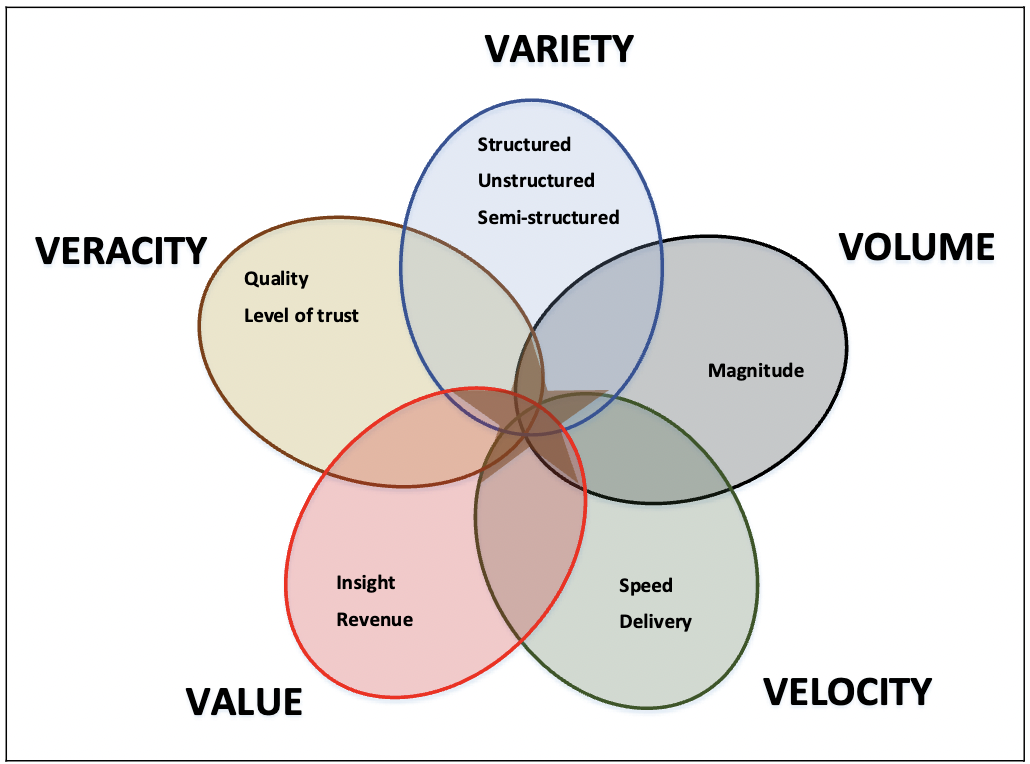
\includegraphics[width=0.8\textwidth]{img/bigdata.png}
    \caption{Mô hình 5V của dữ liệu lớn \cite{Husamaldin2019}}
    \label{fig:bigdata}
    \end{figure}
\vspace*{1ex}
\begin{itemize}
    \item \textbf{Khối lượng (Volume)}: Đề cập đến quy mô dữ liệu cực lớn.
    \item \textbf{Tốc độ (Velocity)}: Tốc độ dữ liệu được tạo ra, truyền tải và xử lý.
    \item \textbf{Tính đa dạng (Variety)}: Nguồn và định dạng dữ liệu đa dạng như văn bản, hình ảnh, video, v.v.
    \item \textbf{Tính xác thực (Veracity)}: Mức độ đáng tin cậy và chất lượng của dữ liệu.
    \item \textbf{Giá trị (Value)}: Tiềm năng khai thác thông tin hữu ích từ dữ liệu.
\end{itemize}

Dữ liệu sinh ra từ các thiết bị \ac{iot} được xem là một trong những nguồn tạo ra dữ liệu lớn (\ac{bd}) quan trọng và phát triển nhanh chóng hiện nay. Với hàng tỷ thiết bị cảm biến, máy móc, thiết bị đeo tay và phương tiện kết nối Internet, lượng dữ liệu được tạo ra mỗi ngày rất lớn, đa dạng về định dạng và tốc độ phát sinh liên tục theo thời gian thực. Dữ liệu \ac{iot} mang đầy đủ các đặc điểm của dữ liệu lớn như: khối lượng (volume) lớn, tốc độ (velocity) cao, tính đa dạng (variety) về loại dữ liệu, mức độ xác thực (veracity) không đồng đều và tiềm năng mang lại giá trị (value) lớn nếu được khai thác hiệu quả. Chính vì vậy, dữ liệu \ac{iot} không chỉ là một phần của dữ liệu lớn mà còn đóng vai trò quan trọng trong việc thúc đẩy nhu cầu phát triển các nền tảng xử lý dữ liệu lớn hiện đại.

\subsection{Các thành phần của Apache Spark}

Trong những năm gần đây, các nền tảng xử lý dữ liệu lớn như Apache Spark đã thu hút sự quan tâm rộng rãi từ cộng đồng nghiên cứu và công nghiệp. Apache Spark là một hệ thống xử lý dữ liệu phân tán quy mô lớn, có khả năng thực thi nhanh các tác vụ trên các cụm dữ liệu lớn. So với Hadoop MapReduce, Spark có thể đạt tốc độ xử lý nhanh hơn khoảng 100 lần trong một số trường hợp nhờ vào khả năng xử lý trong bộ nhớ (\textit{in-memory processing}) \cite{Karau2015}.

Bên cạnh đó, Spark cung cấp giao diện lập trình linh hoạt thông qua các API hỗ trợ nhiều ngôn ngữ phổ biến như Java, Scala, Python và R, giúp việc phát triển và triển khai ứng dụng trở nên thuận tiện hơn.

Apache Spark bao gồm nhiều thành phần chính tạo thành một hệ sinh thái hoàn chỉnh, hỗ trợ đa dạng các tác vụ phân tích dữ liệu như xử lý dữ liệu tuần tự, truy vấn SQL, phân tích luồng dữ liệu thời gian thực, học máy và xử lý đồ thị (Hình~\ref{fig:spark}).

\vspace*{1ex}
    \begin{figure}[ht]
    \centering
    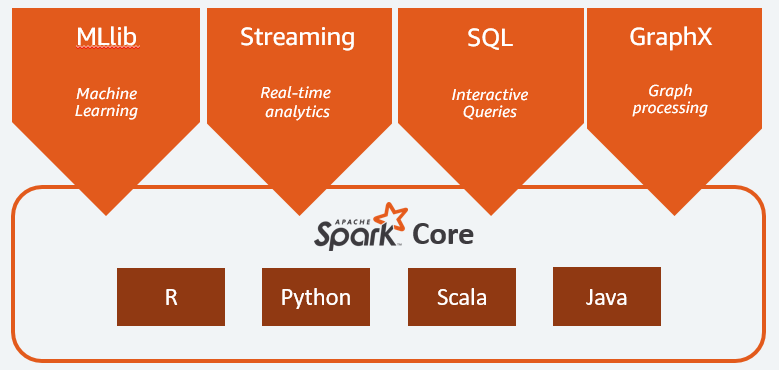
\includegraphics[width=0.8\textwidth]{img/spark.png}
    \caption{Các thành phần của Apache Spark}
    \label{fig:spark}
    \end{figure}
\vspace*{1ex}
Apache Spark bao gồm nhiều thành phần cốt lõi, mỗi thành phần đảm nhận một chức năng cụ thể trong quá trình xử lý dữ liệu lớn:

\begin{itemize}
  \item \textbf{Spark Core}: Thành phần trung tâm của Spark, chịu trách nhiệm quản lý bộ nhớ, lập lịch, xử lý lỗi, phân phối tác vụ và giao tiếp với các hệ thống lưu trữ. Nó cung cấp các API cấp cao cho Java, Scala, Python và R, giúp đơn giản hóa việc xử lý phân tán.

  \item \textbf{MLlib}: Thư viện máy học tích hợp sẵn trong Spark, hỗ trợ huấn luyện và triển khai các mô hình học máy trên quy mô lớn. MLlib cung cấp các thuật toán như phân loại, hồi quy, phân cụm, khai thác mẫu và lọc cộng tác.

  \item \textbf{Spark Streaming}: Công cụ xử lý dữ liệu thời gian thực bằng cách chia dòng dữ liệu thành các lô nhỏ để xử lý tương tự như dữ liệu theo lô. Công cụ này cho phép sử dụng lại mã nguồn và hỗ trợ nhiều nguồn dữ liệu như Kafka, Flume, Twitter, HDFS.

  \item \textbf{Spark SQL}: Thành phần truy vấn dữ liệu phân tán, hỗ trợ ngôn ngữ SQL tiêu chuẩn và HiveQL với hiệu suất cao nhờ tối ưu hóa Catalyst và định dạng cột. Nó hỗ trợ nhiều nguồn dữ liệu như JSON, Hive, Parquet, JDBC, MongoDB, Cassandra.

  \item \textbf{GraphX}: Thư viện xử lý đồ thị phân tán, hỗ trợ biểu diễn, chuyển đổi và phân tích dữ liệu đồ thị. GraphX đi kèm với các thuật toán đồ thị phổ biến như PageRank, Connected Components và nhiều thuật toán phân tích khác.
\end{itemize}

\subsection{Kiến trúc của Apache Spark}
Kiến trúc của Apache Spark được xây dựng theo mô hình master–worker trên nền tảng xử lý phân tán. Thành phần trung tâm là \textbf{Spark Driver}, chịu trách nhiệm điều phối quá trình thực thi ứng dụng, bao gồm việc lên lịch, phân phối tác vụ và giám sát tiến trình. Driver tạo ra một phiên bản logic gọi là \textit{DAG} (Directed Acyclic Graph) để xác định luồng thực thi công việc; tổng quan kiến trúc master--worker được minh họa ở Hình~\ref{fig:spark-structure}.

\vspace*{1ex}
    \begin{figure}[ht]
    \centering
    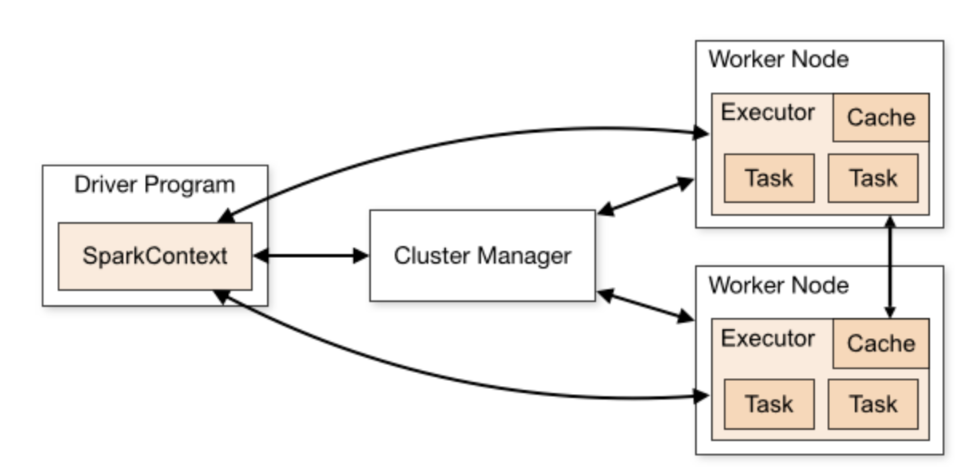
\includegraphics[width=0.85\textwidth]{img/spark-structure.png}
    \caption{Sơ đồ kiến trúc hệ thống Apache Spark}
    \label{fig:spark-structure}
    \end{figure}
\vspace*{1ex}

Các tác vụ được phân phối tới các \textbf{Worker Nodes}, nơi chứa các \textbf{Executor} — tiến trình thực thi thực tế. Mỗi Executor chịu trách nhiệm thực thi các tác vụ (task) và lưu trữ dữ liệu trong bộ nhớ hoặc ổ đĩa nếu cần. Spark sử dụng \textbf{Cluster Manager} (như YARN, Mesos hoặc Standalone) để quản lý tài nguyên trên cụm. Dữ liệu được lưu trữ trên các hệ thống như HDFS, S3, hoặc các cơ sở dữ liệu quan hệ.

\section{Học máy trong phát hiện xâm nhập}

Học máy (\ac{ml}) đã trở thành một công cụ thiết yếu trong việc phát hiện các mẫu tấn công và hành vi bất thường trong lưu lượng mạng \ac{iot}, nhờ khả năng tự động học và thích ứng từ dữ liệu lịch sử \cite{Buczak2016}. Các kỹ thuật học máy phổ biến bao gồm:

\begin{itemize}
\item \textbf{Học có giám sát (Supervised Learning)}: Sử dụng dữ liệu đã được gán nhãn để huấn luyện mô hình phân loại. Một số thuật toán điển hình gồm \ac{rf}, \ac{svm} và Mạng nơ-ron nhân tạo (Neural Networks).
\item \textbf{Học không giám sát (Unsupervised Learning)}: Áp dụng cho các tình huống không có nhãn, tập trung vào việc phát hiện các mẫu bất thường. K-Means là một thuật toán phổ biến trong nhóm này.
\item \textbf{Học tăng cường (Reinforcement Learning)}: Mô hình học dựa trên phản hồi từ môi trường nhằm tối ưu hóa hành vi hoặc quyết định của hệ thống theo thời gian.
\end{itemize}

Trong bối cảnh mạng \ac{iot}, học máy được ứng dụng rộng rãi để phân tích lưu lượng dữ liệu và nhận diện các loại tấn công như DDoS, botnet hay giả mạo gói tin. Theo nghiên cứu của Koroniotis và cộng sự (2020), mô hình \ac{rf} triển khai trên nền tảng Apache Spark đã đạt độ chính xác rất cao khi phát hiện tấn công SYN-DOS, đồng thời đảm bảo tốc độ xử lý cao, phù hợp với yêu cầu thời gian thực của môi trường \ac{iot} \cite{Koroniotis2020}. Tuy nhiên, các kết quả gần như tuyệt đối (xấp xỉ 100\%) trên các tập dữ liệu công khai cần được xem xét thận trọng, vì chúng thường là dấu hiệu của rò rỉ dữ liệu (data leakage) hơn là năng lực thực sự của mô hình. \emph{Rò rỉ dữ liệu} là tình huống trong đó thông tin lẽ ra không sẵn có ở thời điểm triển khai thực tế lại lọt vào quá trình huấn luyện hoặc đánh giá, khiến điểm số bị thổi phồng và không phản ánh đúng khả năng tổng quát hoá của mô hình. Luận văn này nhận diện và xử lý vấn đề đó một cách tường minh ở Chương~\ref{c:thucnghiemdanhgia}.

Tuy nhiên, việc ứng dụng học máy trong hệ thống \ac{iot} vẫn còn gặp nhiều thách thức vì yêu cầu xử lý theo thời gian thực và hạn chế về tài nguyên tính toán. Việc tích hợp học máy với các nền tảng xử lý dữ liệu lớn như Apache Spark mang lại lợi thế đáng kể, giúp xử lý khối lượng dữ liệu lớn với tốc độ cao và hỗ trợ triển khai các thuật toán học máy hiệu quả trong môi trường phân tán.
\subsection{Một số thuật toán học máy}
\begin{itemize}
\item \textbf{Cây quyết định (\ac{dt})} là một trong những thuật toán học máy có giám sát phổ biến, được áp dụng rộng rãi trong các bài toán phân loại. Cấu trúc cơ bản của một cây quyết định bao gồm ba thành phần chính: \textbf{nút gốc}, \textbf{nút quyết định} và \textbf{nút lá}.
Cây quyết định có ưu điểm là dễ hiểu, dễ diễn giải, có thể trực quan hóa và không yêu cầu giả định về phân phối dữ liệu. Tuy nhiên, \ac{dt} cũng dễ bị quá khớp (\textit{overfitting}) nếu không chọn được các tham số hợp lý hoặc xử lý trên dữ liệu nhiễu \cite{mitchell1997machine}.

\item \textbf{Rừng ngẫu nhiên (\ac{rf})} là một thuật toán học máy được sử dụng phổ biến trong cả hai bài toán phân loại và hồi quy. Đây là một kỹ thuật học tập kết hợp (\textit{ensemble learning}) dựa trên việc xây dựng và tổng hợp nhiều cây quyết định độc lập nhằm nâng cao độ chính xác và độ ổn định của mô hình. Thuật toán hoạt động bằng cách tạo ra nhiều cây quyết định trên các tập con khác nhau được chọn ngẫu nhiên từ tập dữ liệu huấn luyện. Mỗi cây được xây dựng dựa trên một mẫu bootstrap (lấy mẫu có hoàn lại), đồng thời tại mỗi nút chia, một tập con ngẫu nhiên của các thuộc tính được chọn để tìm điểm chia tốt nhất, thay vì sử dụng toàn bộ thuộc tính như trong cây quyết định truyền thống \cite{breiman2001random}.

Kết quả cuối cùng được xác định bằng cách:  
\begin{itemize}
    \item Trong bài toán phân loại: lấy kết quả theo nguyên tắc đa số phiếu (\textit{majority voting}) từ các cây.  
    \item Trong bài toán hồi quy: lấy giá trị trung bình từ các dự đoán của từng cây.
\end{itemize}

Việc kết hợp nhiều cây giúp \ac{rf} giảm thiểu hiện tượng quá khớp (\textit{overfitting}) vốn là một nhược điểm thường gặp của các cây quyết định đơn lẻ. Khi số lượng cây trong rừng tăng lên, hiệu suất dự đoán của mô hình có xu hướng ổn định và cải thiện hơn.
\item \textbf{Hồi quy logistic (\ac{lr})} là một phương pháp thống kê được giới thiệu bởi David Cox vào cuối thập niên 1950. Đây là một kỹ thuật học máy có giám sát thường được sử dụng để giải quyết các bài toán phân loại nhị phân, trong đó biến đầu ra (phản hồi) là một biến định tính, nhận giá trị \texttt{0} hoặc \texttt{1}. Mô hình hồi quy logistic cho phép ước tính xác suất xảy ra của một sự kiện cụ thể dựa trên một hoặc nhiều biến đầu vào (độc lập). Một trong những điểm mạnh của phương pháp này là khả năng xác định mức độ ảnh hưởng của từng yếu tố đến xác suất xuất hiện của kết quả, giúp các nhà phân tích hiểu rõ hơn mối quan hệ giữa biến đầu vào và đầu ra \cite{cox1958regression}.

Về mặt toán học, hàm hồi quy logistic được biểu diễn dưới dạng tuyến tính như sau:

\begin{equation}
z_i = \beta_0 + \beta_1 x_{i,1} + \beta_2 x_{i,2} + \cdots + \beta_n x_{i,n}
\label{eq:linear_combination}
\end{equation}

Trong đó:
\begin{itemize}
    \item $x_{i,j}$ là giá trị của biến độc lập thứ $j$ tại quan sát thứ $i$
    \item $\beta_0$ là hệ số chặn (bias), $\beta_j$ là hệ số hồi quy ứng với biến $x_j$
    \item $z_i$ là đầu ra tuyến tính trước khi chuẩn hóa
\end{itemize}

Sau đó, xác suất xảy ra của sự kiện được tính thông qua hàm logistic (sigmoid):
\begin{equation}
P(Y_i = 1 \mid \mathbf{x}_i) = \frac{1}{1 + e^{-z_i}}
\label{eq:sigmoid}
\end{equation}

Trong quá trình huấn luyện, mô hình tìm các hệ số $\beta_j$ tối ưu sao cho hàm mất mát (cross-entropy loss) được tối thiểu hóa.

\item \textbf{\ac{gbt}} là một phương pháp học máy tăng cường (\textit{boosting}) sử dụng các cây quyết định như mô hình học yếu (weak learners). Ý tưởng chính của boosting là xây dựng một mô hình mạnh bằng cách kết hợp nhiều mô hình học yếu được huấn luyện theo trình tự tuần tự. Ở mỗi bước, thuật toán cố gắng giảm thiểu lỗi của mô hình trước bằng cách học từ phần dư (residual) hoặc gradient của hàm mất mát \cite{friedman2001greedy}. Quá trình huấn luyện \ac{gbt} gồm các bước:
\begin{itemize}
    \item Bắt đầu với một mô hình dự đoán ban đầu (thường là giá trị trung bình với bài toán hồi quy).
    \item Tính toán sai số còn lại giữa nhãn thực và dự đoán.
    \item Huấn luyện một cây quyết định để dự đoán phần dư.
    \item Cập nhật mô hình tổng bằng cách cộng mô hình hiện tại với mô hình mới nhân với một hệ số học $\eta$ (learning rate).
\end{itemize}

Giả sử $F_0(x)$ là mô hình khởi tạo ban đầu, mô hình tổng tại bước $m$ được cập nhật theo công thức:

\begin{equation}
F_m(x) = F_{m-1}(x) + \eta \cdot h_m(x)
\end{equation}

Trong đó:
\begin{itemize}
    \item $h_m(x)$ là cây quyết định thứ $m$ học theo gradient của hàm mất mát.
    \item $\eta$ là hệ số học (learning rate), thường $\eta \in (0, 1)$.
\end{itemize}

\item \textbf{\ac{lgbm}} là một framework triển khai thuật toán \ac{gbt}, được phát triển nhằm tối ưu hóa tốc độ huấn luyện và khả năng mở rộng trên các tập dữ liệu lớn \cite{ke2017lightgbm}. Đây là một phương pháp học tập tăng cường (\textit{boosting}) trong đó các cây quyết định được xây dựng tuần tự, mỗi cây mới được huấn luyện để giảm sai số của mô hình trước đó thông qua gradient của hàm mất mát \cite{friedman2001greedy}. 

Giả sử $F_0(x)$ là mô hình khởi tạo ban đầu, mô hình tại bước $m$ được cập nhật như sau:

\begin{equation}
F_m(x) = F_{m-1}(x) + \eta h_m(x)
\end{equation}

Trong đó:
\begin{itemize}
    \item $h_m(x)$ là cây quyết định thứ $m$ học theo gradient của hàm mất mát,
    \item $\eta$ là hệ số học (\textit{learning rate}), thường $\eta \in (0,1)$.
\end{itemize}

Khác với \ac{gbt} truyền thống, \ac{lgbm} sử dụng cơ chế phát triển cây theo hướng leaf-wise thay vì level-wise, đồng thời áp dụng thuật toán histogram-based splitting và kỹ thuật Gradient-based One-Side Sampling (GOSS) nhằm giảm chi phí tính toán và tăng tốc độ huấn luyện. Tuy nhiên, do thư viện gốc của \ac{lgbm} (thông qua SynapseML) chỉ hỗ trợ kiến trúc x86\_64 và không chạy được trên thiết bị biên ARM (Jetson Orin Nano Super) — mục tiêu triển khai của luận văn — nên \ac{lgbm} \emph{không} được đưa vào bộ thuật toán so sánh thực nghiệm; XGBoost và GBT đại diện cho họ gradient boosting.

\item \textbf{\ac{nb}} là một phương pháp phân loại xác suất dựa trên định lý Bayes với giả định độc lập có điều kiện giữa các đặc trưng \cite{mccallum1998comparison}. Mặc dù giả định này thường không hoàn toàn đúng trong thực tế, mô hình vẫn cho hiệu quả tốt trong nhiều bài toán phân loại dữ liệu nhiều chiều.

Theo định lý Bayes:

\begin{equation}
P(y|x) = \frac{P(x|y)P(y)}{P(x)}
\end{equation}

Với giả định độc lập giữa các đặc trưng:

\begin{equation}
P(x|y) = \prod_{i=1}^{n} P(x_i|y)
\end{equation}

Mô hình lựa chọn lớp có xác suất hậu nghiệm lớn nhất:

\begin{equation}
\hat{y} = \arg\max_y P(y)\prod_{i=1}^{n} P(x_i|y)
\end{equation}

Ưu điểm của \ac{nb} là đơn giản, tốc độ huấn luyện nhanh và phù hợp với dữ liệu kích thước lớn; tuy nhiên, hạn chế chính nằm ở giả định độc lập giữa các đặc trưng.

\item \textbf{Support Vector Machine (\ac{svm})} là một thuật toán học có giám sát được đề xuất bởi Cortes và Vapnik \cite{cortes1995support}, nhằm tìm siêu phẳng tối ưu phân tách dữ liệu với khoảng cách biên (margin) lớn nhất. 

Trong trường hợp dữ liệu tuyến tính, bài toán tối ưu được biểu diễn như sau:

\begin{equation}
\min_{w,b} \frac{1}{2} ||w||^2
\end{equation}

với điều kiện:

\begin{equation}
y_i(w \cdot x_i + b) \ge 1
\end{equation}

Trong trường hợp dữ liệu không tuyến tính, \ac{svm} sử dụng kỹ thuật \textit{kernel trick} để ánh xạ dữ liệu sang không gian chiều cao hơn, cho phép phân tách tuyến tính trong không gian mới. Nhờ cơ chế tối ưu hóa chặt chẽ, \ac{svm} thường đạt hiệu suất cao trong các bài toán phân loại với dữ liệu chiều cao.

\item \textbf{Multilayer Perceptron - MLP} là một mô hình học sâu cơ bản gồm nhiều lớp ẩn, có khả năng mô hình hóa các mối quan hệ phi tuyến giữa các đặc trưng \cite{rumelhart1986learning}. 

Mỗi neuron trong mạng thực hiện phép biến đổi tuyến tính:

\begin{equation}
z = w^T x + b
\end{equation}

sau đó áp dụng hàm kích hoạt phi tuyến:

\begin{equation}
a = \sigma(z)
\end{equation}

Trong đó $\sigma(\cdot)$ có thể là các hàm kích hoạt như sigmoid, tanh hoặc ReLU. Quá trình huấn luyện sử dụng thuật toán lan truyền ngược (\textit{backpropagation}) nhằm cập nhật trọng số thông qua tối thiểu hóa hàm mất mát bằng gradient descent. MLP có khả năng biểu diễn mạnh nhưng yêu cầu dữ liệu huấn luyện đủ lớn và quá trình điều chỉnh siêu tham số cẩn thận để tránh hiện tượng quá khớp.

\item \textbf{\ac{xgb}} là một phiên bản cải tiến của thuật toán \ac{gbt} truyền thống, được đề xuất bởi Chen và Guestrin vào năm 2016. \ac{xgb} được thiết kế để tối ưu hóa tốc độ huấn luyện, hiệu suất mô hình, và khả năng xử lý dữ liệu quy mô lớn trong các hệ thống tính toán phân tán \cite{chen2016xgboost}. \ac{xgb} sử dụng các chiến lược sau để cải thiện hiệu năng:
\begin{itemize}
    \item Ánh xạ gradient và Hessian để tối ưu hóa hiệu quả (second-order optimization).
    \item Cắt tỉa cây (pruning) theo độ phức tạp thay vì độ sâu cố định.
    \item Tính song song trong việc tìm điểm chia tối ưu (split finding).
    \item Hỗ trợ xử lý thiếu giá trị (missing values) tự động.
\end{itemize}

Mô hình \ac{xgb} đã được ứng dụng thành công trong nhiều bài toán học máy thực tế như dự báo tài chính, chẩn đoán y tế, phát hiện gian lận và phân tích hành vi khách hàng, nhờ độ chính xác cao và hiệu quả tính toán tốt.
\end{itemize}
\subsection{Một số thuật toán Ensemble learning}
\textbf{Ensemble Learning (\ac{el})} là một kỹ thuật trong học máy nhằm kết hợp nhiều mô hình riêng lẻ để nâng cao độ chính xác và độ ổn định trong dự đoán. Thay vì chỉ dựa vào một mô hình đơn lẻ, phương pháp \ac{el} tận dụng sức mạnh tổng hợp của nhiều mô hình — ví dụ như \ac{dt}, \ac{rf}, \ac{lr}, v.v. --- để xây dựng một hệ thống dự đoán chính xác hơn. Nguyên lý cốt lõi của \ac{el} là: mỗi mô hình riêng lẻ có thể chỉ đạt độ chính xác thấp hoặc dự đoán sai ở một số trường hợp, nhưng sự kết hợp hợp lý của chúng có thể giảm thiểu sai số, tăng độ chính xác nhờ tận dụng điểm mạnh và khắc phục điểm yếu của từng mô hình thành phần \cite{zhou2012ensemble}.

Kỹ thuật \ac{el} đã chứng minh được tính hiệu quả cao trong nhiều lĩnh vực yêu cầu độ chính xác cao như: phát hiện gian lận, phân tích dữ liệu lớn, nhận diện hình ảnh và xử lý ngôn ngữ tự nhiên. Trong lĩnh vực bảo mật mạng \ac{iot}, \ac{el} cũng được ứng dụng để cải thiện khả năng phát hiện bất thường hoặc xâm nhập dựa trên nhiều mô hình học máy được huấn luyện song song hoặc tuần tự.

Một số phương pháp phổ biến của \ac{el} bao gồm:
\begin{itemize}
    \item \textbf{Voting}: Với bài toán phân loại, mỗi mô hình con bỏ phiếu cho một lớp và lớp có số phiếu cao nhất sẽ là đầu ra cuối cùng (đa số phiếu hoặc trung bình xác suất). Các bước của voting được mô tả chi tiết ở Thuật toán~\ref{voting_ag1}.
    \item \textbf{Boosting}: Huấn luyện các mô hình tuần tự, trong đó mỗi mô hình mới tập trung vào các mẫu mà mô hình trước đã dự đoán sai (ví dụ: \ac{gbt}, AdaBoost, \ac{xgb}). Các bước của boosting được mô tả chi tiết ở Thuật toán~\ref{boosting_ag1}.
    \item \textbf{Bagging (Bootstrap Aggregating)}: Huấn luyện nhiều mô hình trên các tập con ngẫu nhiên (lấy mẫu có hoàn lại) của tập dữ liệu gốc, sau đó tổng hợp kết quả dự đoán (ví dụ: Random Forest). Các bước của bagging được mô tả chi tiết ở Thuật toán~\ref{bagging_ag1}.
\end{itemize}

\ac{el} đặc biệt hữu ích trong các hệ thống phát hiện xâm nhập (\ac{ids}) vì cần phân tích lượng lớn dữ liệu phức tạp, và việc kết hợp nhiều mô hình có thể giúp tăng khả năng phát hiện các gói tin bất thường mà một mô hình đơn lẻ có thể bỏ sót.

\begin{algorithm}[htbp]
\caption{Voting: Kết hợp dự đoán từ nhiều mô hình phân loại}
\label{voting_ag1}
\textbf{Đầu vào:}
\begin{itemize}
  \item Tập huấn luyện $\mathcal{D} = \{(x_i, y_i)\}_{i=1}^N$
  \item Tập mô hình phân loại cơ sở $M_1, M_2, \dots, M_K$
  \item Kiểu voting: \texttt{HARD} hoặc \texttt{SOFT}
\end{itemize}

\textbf{Đầu ra:} Nhãn dự đoán cuối cùng $y_{\text{vote}}$ cho điểm dữ liệu $x$

\begin{algorithmic}[1]
\State \textbf{Khởi tạo:} danh sách $S = \{\}$ \Comment{Lưu dự đoán hoặc xác suất}
\If{voting = \texttt{HARD}}
    \For{$j = 1$ to $K$}
        \State $y_j \gets M_j(x)$ \Comment{Dự đoán nhãn của mô hình thứ $j$}
        \State Thêm $y_j$ vào $S$
    \EndFor
    \State $y_{\text{vote}} \gets$ nhãn xuất hiện nhiều nhất trong $S$
\ElsIf{voting = \texttt{SOFT}}
    \State Khởi tạo xác suất tổng $P_{\text{sum}}[c] = 0, \forall c \in \{1, \dots, C\}$
    \For{$j = 1$ to $K$}
        \State Lấy xác suất $P_j(y = c \mid x)$ từ mô hình $M_j$
        \For{mỗi lớp $c = 1$ to $C$}
            \State $P_{\text{sum}}[c] \gets P_{\text{sum}}[c] + P_j(y = c \mid x)$
        \EndFor
    \EndFor
    \State $y_{\text{vote}} \gets \arg\max_{c} P_{\text{sum}}[c]$
\EndIf
\State \Return $y_{\text{vote}}$
\end{algorithmic}
\end{algorithm}

\begin{algorithm}[htbp]
\caption{Boosting: Học tăng cường tuần tự}
\label{boosting_ag1}
\textbf{Đầu vào:}
\begin{itemize}
  \item Tập dữ liệu huấn luyện $\mathcal{D} = \{(x_i, y_i)\}_{i=1}^N$
  \item Số lượng vòng lặp (mô hình yếu): $T$
\end{itemize}

\textbf{Đầu ra:} Mô hình tăng cường $F_T(x)$

\begin{algorithmic}[1]
\State \textbf{Khởi tạo:} $F_0(x) \gets 0$ \Comment{Mô hình khởi đầu có thể là 0 hoặc dự đoán trung bình}
\For{$t = 1$ to $T$}
    \State Tính phần dư (residuals) cho từng mẫu: $r_i^{(t)} = y_i - F_{t-1}(x_i)$
    \State Huấn luyện mô hình yếu $h_t(x)$ trên các phần dư $r_i^{(t)}$
    \State Cập nhật mô hình: $F_t(x) = F_{t-1}(x) + \eta \cdot h_t(x)$
\EndFor
\State \Return $F_T(x)$
\end{algorithmic}
\end{algorithm}

\begin{algorithm}[htbp]
\caption{Bagging: Bootstrap Aggregating}
\label{bagging_ag1}
\textbf{Đầu vào:}
\begin{itemize}
  \item Tập huấn luyện $\mathcal{D} = \{(x_i, y_i)\}_{i=1}^N$, với $x_i \in \mathbb{R}^d$, $y_i \in \{1, 2, \dots, C\}$
  \item Số lượng mô hình cơ sở: $K$
\end{itemize}

\textbf{Đầu ra:} Dự đoán cuối cùng $y_{\text{bag}}$ cho một điểm dữ liệu $x$

\noindent
\begin{algorithmic}[1]
\State \textbf{Khởi tạo:} Danh sách mô hình $M_1, M_2, \dots, M_K$

\For{$k = 1$ to $K$}
  \State Tạo mẫu bootstrap $\mathcal{D}^{(k)}$ từ $\mathcal{D}$ (lấy mẫu ngẫu nhiên có hoàn lại)
  \State Huấn luyện mô hình $M_k \gets \text{Train}(\mathcal{D}^{(k)})$
\EndFor

\State \textbf{Khởi tạo:} Danh sách dự đoán $Y = \{\}$

\For{$k = 1$ to $K$}
  \State Thực hiện dự đoán $y_k \gets M_k(x)$
  \State Thêm $y_k$ vào $Y$
\EndFor

\State Tính $y_{\text{bag}} \gets \text{Voting}(Y)$ \Comment{Hard voting hoặc trung bình xác suất nếu dùng soft}

\State \Return $y_{\text{bag}}$
\end{algorithmic}
\end{algorithm}

\pagebreak



\chapter{Phương pháp thực hiện}
\label{c:phuongphapthuchien}


Trong chương này, luận văn sẽ trình bày phương pháp đề xuất để xây dựng mô hình phát hiện xâm nhập dựa trên Apache Spark cho bảo mật mạng \ac{iot}. Quá trình thực hiện bao gồm 6 bước chính, được thể hiện qua Hình~\ref{fig:training_model}: (1) Thu thập dữ liệu và tiền xử lý; (2) Xây dựng đặc trưng và lựa chọn đặc trưng; (3) Huấn luyện mô hình; (4) Đánh giá mô hình; (5) Tối ưu siêu tham số; và (6) Triển khai biên thời gian thực. Các bước (1)–(5) được lặp lại tương ứng với từng phương pháp lựa chọn đặc trưng (\ac{rfi}, \ac{shap}, \ac{pca}), sau đó lựa chọn mô hình tốt nhất để triển khai trên thiết bị biên.

\begin{figure}[htbp]
    \centering
    \resizebox{0.98\textwidth}{!}{%
    \begin{tikzpicture}[
        font=\small, >=Stealth,
        every node/.style={align=center},
        io/.style ={draw=gray!60,        thick, rounded corners, fill=gray!8,   text width=8.6cm, minimum height=1.0cm, inner sep=3pt},
        ml/.style ={draw=accBlue,        thick, rounded corners, fill=accBlue!5,   text width=8.6cm, minimum height=1.0cm, inner sep=3pt},
        dep/.style={draw=accOrange,thick, rounded corners, fill=accOrange!10,text width=8.6cm, minimum height=1.0cm, inner sep=3pt},
        arr/.style ={-{Stealth[length=2.5mm]}, thick, draw=gray!60!black},
        loop/.style={-{Stealth[length=2.5mm]}, thick, draw=accOrange, dashed},
    ]
        \node[io]  (data)  at (0, 0.0)  {\textbf{(1) Thu thập \& Tiền xử lý}: CICIDS2017\\
            loại trừ rò rỉ dữ liệu (bỏ \texttt{destination\_port}, loại bỏ trùng lặp đặc trưng), chia 80/20};
        \node[ml]  (feat)  at (0,-1.7)  {\textbf{(2) Xây dựng \& lựa chọn đặc trưng}\\
            RF Importance \;$|$\; SHAP \;$|$\; PCA};
        \node[ml]  (train) at (0,-3.4)  {\textbf{(3) Huấn luyện mô hình}: Apache Spark ML\\
            8 thuật toán + Ensemble (Bagging / Voting)};
        \node[ml]  (eval)  at (0,-5.1)  {\textbf{(4) Đánh giá mô hình}\\
            Accuracy, Precision, Recall, F1, AUC-PR + kiểm định thống kê};
        \node[ml]  (tune)  at (0,-6.8)  {\textbf{(5) Tối ưu siêu tham số}\\
            Grid Search + Cross-Validation};
        \node[dep] (dep)   at (0,-8.5)  {\textbf{(6) Triển khai biên thời gian thực}\\
            Chọn mô hình tốt nhất $\rightarrow$ cụm 2 Jetson Orin Nano Super};

        \foreach \a/\b in {data/feat, feat/train, train/eval, eval/tune, tune/dep}
            \draw[arr] (\a) -- (\b);

        % Vòng lặp (2)--(5) theo từng phương pháp lựa chọn đặc trưng
        \draw[loop] (tune.east) -- ++(0.7,0) |- (feat.east);
        \node[anchor=west, font=\footnotesize, text width=2.6cm, text=orange!60!black]
            at (5.1,-4.25) {Lặp lại theo từng phương pháp (RFI / SHAP / PCA)};
        % Điểm ảo cân đối bên trái để cột hộp căn giữa trang (bù nhãn vòng lặp bên phải)
        \path (-7.7,-4.25) rectangle (-7.6,-4.24);
    \end{tikzpicture}}
    \caption{Quy trình tổng thể huấn luyện, đánh giá và triển khai mô hình đề xuất}
    \label{fig:training_model}
\end{figure}

\section{Thu thập dữ liệu và tiền xử lý}
Trong nghiên cứu này, tập dữ liệu được sử dụng là CICIDS2017 được phát hành bởi Viện An ninh mạng Canada (CIC). Tập dữ liệu này được xây dựng nhằm mô phỏng lưu lượng mạng thực tế kết hợp với nhiều loại tấn công mạng hiện đại, phục vụ cho việc huấn luyện và đánh giá các mô hình phát hiện xâm nhập. Tập dữ liệu CICIDS2017 tập trung vào các kịch bản tấn công đơn lẻ trong môi trường kiểm soát. Cần lưu ý rằng các bộ dữ liệu phát hiện xâm nhập mạng công khai --- bao gồm CICIDS2017 --- có những giới hạn đã được khảo sát một cách hệ thống (lỗi gán nhãn, tạo tác khi sinh lưu lượng, và khả năng tổng quát hóa hạn chế)~\cite{goldschmidt2025datasets}; đây là lý do luận văn áp dụng quy trình loại trừ rò rỉ ở bước tiền xử lý và bổ sung đánh giá liên bộ dữ liệu ở Chương~\ref{c:thucnghiemdanhgia}. Thông tin chi tiết về tập dữ liệu được trình bày trong Bảng~\ref{tab:cicids2017}.

\begin{table}[htbp]
\centering
\caption{Mô tả bộ dữ liệu CICIDS2017}
\label{tab:cicids2017}
\renewcommand{\arraystretch}{1.1}
\begin{tabular}{l@{\hspace{10pt}}>{\raggedright\arraybackslash}p{10cm}}
\toprule
\textbf{Thuộc tính}              & \textbf{Giá trị} \\
\midrule
Tổ chức phát hành                & Canadian Institute for Cybersecurity (CIC) \\
Thời gian phát hành              & 2017 \\
Giao thức mạng                   & HTTP, HTTPS, FTP, SSH, DNS, ... \\
Số lượng bản ghi (CSV)           & Hơn 2.8 triệu bản ghi \\
Thời gian thu thập               & 03/07/2017 – 07/07/2017 \\
Loại tấn công mô phỏng           & DoS, DDoS, PortScan, Brute-force, Infiltration, Botnet, ... \\
Số loại nhãn                     & 15 (1 nhãn bình thường + 14 loại tấn công) \\
Định dạng dữ liệu                & CSV \\
Mục đích                         & Phát hiện xâm nhập mạng trong môi trường thực tế giả lập \\
Nguồn dữ liệu                    & \cite{sharafaldin2018toward} \\
\bottomrule
\end{tabular}
\end{table}

Bên cạnh CICIDS2017 (bộ dữ liệu chính cho toàn bộ các thí nghiệm), luận văn sử dụng thêm \textbf{CSE-CIC-IDS2018} cho thí nghiệm \emph{tổng quát hóa liên bộ dữ liệu} (Mục~\ref{sec:cross-dataset}): huấn luyện trên một bộ, kiểm tra trên bộ kia và ngược lại. Đây là bộ kế nhiệm của CICIDS2017, do CIC phối hợp với Cơ quan An ninh Truyền thông Canada (CSE) thu thập trên hạ tầng AWS quy mô lớn hơn nhiều; đặc trưng luồng được trích bằng CICFlowMeter phiên bản mới hơn nên tên cột được ánh xạ về danh mục tên cột chuẩn của CICIDS2017 qua bảng bí danh tường minh trong mã nguồn. Thông tin chi tiết ở Bảng~\ref{tab:cicids2018}.

\begin{table}[htbp]
\centering
\caption{Mô tả bộ dữ liệu CSE-CIC-IDS2018 (dùng cho thí nghiệm liên bộ dữ liệu)}
\label{tab:cicids2018}
\renewcommand{\arraystretch}{1.1}
\small
\begin{tabular}{l@{\hspace{10pt}}>{\raggedright\arraybackslash}p{9cm}}
\toprule
\textbf{Thuộc tính}              & \textbf{Giá trị} \\
\midrule
Tổ chức phát hành                & CIC phối hợp CSE (Communications Security Establishment) \\
Thời gian phát hành              & 2018 \\
Hạ tầng thu thập                 & Testbed trên AWS ($\sim$450 máy nạn nhân, 50 máy tấn công) \\
Số lượng bản ghi (CSV)           & $\sim$16{,}2 triệu luồng (10 tệp CSV theo ngày) \\
Thời gian thu thập               & 14/02/2018 -- 02/03/2018 \\
Loại tấn công mô phỏng           & DDoS (HOIC, LOIC-HTTP/UDP), DoS (Hulk, GoldenEye, Slowloris, SlowHTTPTest), Bot, Brute-force (SSH, FTP, Web, XSS), SQL Injection, Infiltration \\
Số loại nhãn                     & 15 (1 nhãn bình thường + 14 loại tấn công) \\
Phân bố nhị phân (sau làm sạch)  & $\sim$13{,}35 triệu Benign / $\sim$2{,}35 triệu Attack \\
Phần dùng trong luận văn          & Mẫu phân tầng theo nhãn 20\% (\texttt{seed}=42), còn $\sim$2{,}39 triệu luồng sau khử trùng lặp mức đặc trưng \\
Định dạng dữ liệu                & CSV (CICFlowMeter v3; tên cột ánh xạ về chuẩn CICIDS2017) \\
Nguồn dữ liệu                    & \cite{CSECICIDS2018} \\
\bottomrule
\end{tabular}
\end{table}

\break

\textbf{Tiền xử lý dữ liệu}
Việc tiền xử lý dữ liệu nhằm loại bỏ nhiễu, giá trị ngoại lệ và giá trị bị thiếu được thực hiện trước khi đưa dữ liệu vào huấn luyện mô hình. Các kỹ thuật được áp dụng gồm chuẩn hóa tên cột, căn chỉnh lược đồ giữa các tệp, thay thế giá trị vô cùng, loại bỏ bản ghi trùng lặp/thiếu, và gán nhãn nhị phân (BENIGN $=0$, Attack $=1$).

Bên cạnh đó, để bảo đảm kết quả đánh giá phản ánh đúng năng lực mô hình, luận văn áp dụng thêm hai bước \emph{loại trừ rò rỉ dữ liệu} (loại cạm bẫy ``data snooping'' được xem là phổ biến nhất của học máy trong an ninh~\cite{arp2022dosdonts}) ngay trong giai đoạn tiền xử lý, trước khi phân chia tập: (i) \textbf{loại đặc trưng rò rỉ nhãn} \texttt{destination\_port} (và \texttt{source\_port} nếu có) — vì trong CICIDS2017, mỗi loại tấn công được sinh nhằm vào những cổng dịch vụ cố định nên cổng đích gần như mã hóa trực tiếp nhãn, khiến mô hình ``ghi nhớ'' ánh xạ cổng--nhãn thay vì học hành vi luồng (cột \texttt{protocol} cũng được loại với lý do tương tự: đây là biến phân loại có ít mức giá trị, tương quan mạnh với cổng dịch vụ nên mang cùng nguy cơ ``lối tắt'' định danh dịch vụ thay vì hành vi); và (ii) \textbf{loại bỏ trùng lặp ở mức đặc trưng theo cơ chế tất định} — các luồng được gom nhóm theo toàn bộ vector đặc trưng; với nhóm có nhãn nhất quán, giữ lại đúng một đại diện; với nhóm trùng đặc trưng nhưng \emph{mâu thuẫn nhãn} (cùng vector đặc trưng, nhãn vừa Benign vừa Attack, một lỗi gán nhãn đã được ghi nhận của CICIDS2017~\cite{lanvin2023errors}), \emph{toàn bộ nhóm bị loại} vì không thể xác định nhãn đúng, thay vì giữ lại một hàng tùy ý theo phân mảnh dữ liệu (vốn không tái lập được giữa các lần chạy); số nhóm và số hàng xung đột nhãn được ghi log tường minh (270 nhóm, 44.260 hàng). Cơ chế này tránh việc cùng một mẫu xuất hiện ở cả tập huấn luyện lẫn kiểm tra khi phân chia ngẫu nhiên. Đối với tập dữ liệu CICIDS2017, quá trình tiền xử lý dữ liệu được thể hiện chi tiết ở Thuật toán~\ref{data_preparation_ag}. Cần thừa nhận rằng bước loại bỏ trùng lặp ở mức đặc trưng làm \emph{thay đổi phân bố lớp}: do các luồng benign trùng lặp nhiều hơn nên bị loại nhiều hơn, khiến tỷ lệ benign/attack sau khi xử lý khác với tỷ lệ ban đầu; vì vậy phân bố lớp trước và sau khi loại trùng lặp được báo cáo tường minh để bảo đảm minh bạch.

\begin{algorithm}[htbp]
\caption{Thuật toán Tiền xử lý Dữ liệu CICIDS2017}
\label{data_preparation_ag}
\begin{algorithmic}[1]
\Require Tập $N$ tệp CSV từ bộ dữ liệu CICIDS2017: $\{F_1, F_2, \dots, F_N\}$
\Statex \qquad Tỷ lệ phân chia huấn luyện/kiểm tra $\alpha = 0.8$
\Ensure Tập huấn luyện $D_{\text{train}}$ và tập kiểm tra $D_{\text{test}}$ ở định dạng Parquet

\State \textbf{Bước 1: Gộp dữ liệu từ nhiều tệp CSV}
\State $D \gets \emptyset$
\For{$i = 1$ to $N$}
    \State Đọc tệp $F_i$ thành DataFrame $df_i$ với lược đồ suy luận tự động
    \State \Call{CleanColumnNames}{$df_i$} \Comment{Chuẩn hóa tên cột: xóa khoảng trắng, chuyển chữ thường}
    \State \Call{HandleInfinityValues}{$df_i$} \Comment{Thay thế $\pm\infty$ bằng giá trị NaN}
    \If{$D = \emptyset$}
        \State $\mathcal{S} \gets \text{Schema}(df_i)$ \Comment{Lưu lược đồ chuẩn từ tệp đầu tiên}
        \State $D \gets df_i$
    \Else
        \State \Call{AlignSchema}{$df_i, \mathcal{S}$} \Comment{Căn chỉnh lược đồ về chuẩn $\mathcal{S}$}
        \State $D \gets D \cup df_i$ \Comment{Gộp theo tên cột (unionByName)}
    \EndIf
\EndFor

\State \textbf{Bước 2: Làm sạch dữ liệu}
\State $D \gets \text{RemoveDuplicates}(D)$ \Comment{Loại bỏ các bản ghi trùng lặp hoàn toàn (giống hệt trên mọi cột)}
\State $D \gets \text{RemoveNulls}(D)$ \Comment{Loại bỏ các bản ghi chứa giá trị null/NaN}

\State \textbf{Bước 3: Tạo nhãn nhị phân}
\State $\forall (x_i, \text{label}_i) \in D: \ y_i \gets \begin{cases} 0 & \text{nếu label}_i = \text{``BENIGN''} \\ 1 & \text{ngược lại (Attack)} \end{cases}$

\Statex \textcolor{accOrange}{\textbf{$\rightarrow$ Hai bước loại trừ rò rỉ dữ liệu (data leakage): Bước 4 và Bước 4b}}
\State \textbf{Bước 4 [loại rò rỉ~--~I]: Xác định các đặc trưng số (đã loại trừ rò rỉ)}
\State $\mathcal{C}_{\text{exclude}} \gets \{\text{label, label\_binary, source\_ip, destination\_ip, flow\_id, timestamp, protocol,}$
\Statex \qquad\qquad $\text{\textbf{destination\_port, source\_port}}\}$ \Comment{Loại bỏ đặc trưng gây rò rỉ nhãn}
\State $\mathcal{F} \gets \{c \in \text{columns}(D) \mid c \notin \mathcal{C}_{\text{exclude}} \wedge \text{dtype}(c) \in \{\text{double, float, int, bigint}\}\}$
\State \textbf{Bước 4b [loại rò rỉ~--~II]: Loại bỏ trùng lặp ở mức đặc trưng (tất định)}
\State $G \gets \text{GroupBy}(D, \mathcal{F})$ \Comment{Gom nhóm theo toàn bộ vector đặc trưng}
\For{mỗi nhóm $g \in G$}
    \If{$|\{y_i : (x_i, y_i) \in g\}| > 1$} \Comment{Nhóm mâu thuẫn nhãn (Benign lẫn Attack)}
        \State Loại toàn bộ nhóm $g$ khỏi $D$; ghi log số nhóm/hàng xung đột
    \Else
        \State Giữ lại đúng một đại diện của $g$ (thứ tự tất định theo nhãn)
    \EndIf
\EndFor

\State \textbf{Bước 5: Phân chia và lưu trữ}
\State $D_{\text{train}}, D_{\text{test}} \gets \text{RandomSplit}(D, [\alpha, 1 - \alpha], \text{seed} = 42)$
\State Lưu $D_{\text{train}}, D_{\text{test}}$ dưới định dạng Parquet
\State \Return $D_{\text{train}}, D_{\text{test}}$
\end{algorithmic}
\end{algorithm}

\textbf{Phân chia tập dữ liệu}

Tập dữ liệu CICIDS2017 được phân chia theo tỷ lệ 80/20 cho huấn luyện và kiểm tra bằng phép chia ngẫu nhiên (random split) với seed cố định (=42) để đảm bảo tái lập. Các chỉ số hiệu năng được \textbf{công bố trên tập kiểm tra} (tập giữ lại cuối cùng, không tham gia huấn luyện, xếp hạng đặc trưng hay tinh chỉnh siêu tham số); kết quả trên tập huấn luyện chỉ được dùng để chẩn đoán hiện tượng quá khớp (overfitting) hoặc thiếu khớp (underfitting). Đáng lưu ý, \texttt{StandardScaler}, \ac{pca} và việc xếp hạng đặc trưng (RF Importance, \ac{shap}) đều được \emph{fit chỉ trên tập huấn luyện $D_{\text{train}}$} rồi \emph{transform} lên tập kiểm tra, nhằm tránh rò rỉ thông tin từ tập kiểm tra vào quá trình huấn luyện. Riêng việc \textbf{chọn Top-3 mô hình thành phần} cho các ensemble (cũng như việc chọn mô hình đại diện mỗi phương pháp và cặp phương pháp đưa vào kiểm định thống kê, Chương~4) được thực hiện trên một \emph{tập kiểm định (validation)} tách từ tập huấn luyện (theo tỷ lệ 80/20, \texttt{seed}=42, các mô hình cơ sở huấn luyện trên phần còn lại); nhờ vậy tập kiểm tra hoàn toàn không tham gia vào khâu lựa chọn mô hình, khép kín nguy cơ rò rỉ chọn lọc. Tương tự, ngưỡng của cổng phát hiện bất thường (Chương~4) cũng chỉ được chọn trên 10\% lưu lượng benign tách từ tập huấn luyện (\texttt{seed}=42), không đụng đến tập kiểm tra. Toàn bộ quy trình phân chia được minh họa ở Hình~\ref{fig:data_split}.

\begin{figure}[htbp]
    \centering
    \resizebox{\textwidth}{!}{%
    \begin{tikzpicture}[
        box/.style ={draw, thick, rounded corners, align=center, minimum height=0.95cm, inner sep=4pt, font=\small},
        arr/.style ={-{Stealth[length=2.4mm]}, thick, draw=gray!55!black},
        lbl/.style ={font=\footnotesize\itshape, text=gray!40!black, fill=white, inner sep=1.5pt},
    ]
        \node[box, draw=gray!55!black, fill=gray!8,       text width=2.7cm] (raw)   at (0,0)      {CICIDS2017 thô\\(tệp CSV)};
        \node[box, draw=accOrange,      fill=accOrange!12, text width=3.1cm] (prep)  at (4.2,0)    {Tiền xử lý\\\textbf{+ loại trừ rò rỉ}\\(Thuật toán~\ref{data_preparation_ag})};
        \node[box, draw=gray!55!black,  fill=gray!8,       text width=1.9cm] (clean) at (8.2,0)    {$D$ sạch};
        \draw[arr] (raw)  -- (prep);
        \draw[arr] (prep) -- (clean);

        \node[box, draw=accBlue,   fill=accBlue!8,    text width=2.5cm] (train) at (12.4,1.4)  {\textbf{Train} (80\%)};
        \node[box, draw=accOrange, fill=accOrange!16, text width=3.3cm] (test)  at (12.4,-1.4) {\textbf{Test} (20\%)\\{\footnotesize giữ lại --- chỉ công bố cuối}};
        \draw[arr] (clean.east) -- ++(0.5,0) |- (train.west);
        \draw[arr] (clean.east) -- ++(0.5,0) |- (test.west);
        \node[lbl, rotate=90, font=\scriptsize\itshape] at (9.79,0) {RandomSplit 80/20, seed=42};

        \node[box, draw=accBlue,  fill=accBlue!8,   text width=3.6cm] (base) at (17.6,2.5) {\textbf{Base-train} (64\%)\\{\footnotesize huấn luyện mô hình cơ sở (để chọn Top-3)}};
        \node[box, draw=accGreen, fill=accGreen!14, text width=3.6cm] (val)  at (17.6,0.3) {\textbf{Validation} (16\%)\\{\footnotesize chọn Top-3 / cặp phương pháp so sánh}};
        \draw[arr] (train.east) -- ++(0.5,0) |- (base.west);
        \draw[arr] (train.east) -- ++(0.5,0) |- (val.west);
        \node[lbl, rotate=90, font=\scriptsize\itshape] at (14.29,1.4) {80/20, seed=42};
    \end{tikzpicture}}
    \caption[Sơ đồ phân chia dữ liệu CICIDS2017]{Sơ đồ phân chia dữ liệu CICIDS2017 (train/test 80/20, \texttt{seed}=42; train tách tiếp 80/20 thành base-train/validation)}
    \label{fig:data_split}
\end{figure}


\section{Lựa chọn đặc trưng và giảm chiều dữ liệu}

Trong quá trình tiền xử lý dữ liệu cho bài toán phát hiện xâm nhập mạng, lựa chọn đặc trưng bao gồm \textbf{chọn đặc trưng} và \textbf{trích xuất đặc trưng} là một bước quan trọng nhằm giảm chiều dữ liệu, loại bỏ những đặc trưng không cần thiết, và cải thiện hiệu năng của mô hình học máy \cite{guyon2003introduction}. Dữ liệu số được gom vào vector đặc trưng bằng \texttt{VectorAssembler} (khoảng 78 đặc trưng số trước khi loại cổng; số đặc trưng chính xác sau khi loại \texttt{destination\_port}/\texttt{source\_port} là 77) và được chuẩn hóa bằng \texttt{StandardScaler} (chuẩn hóa Z-score). Ba phương pháp được sử dụng trong luận văn là \textit{\ac{rf}}, \ac{shap} và \ac{pca}.

\begin{enumerate}[label=\alph*)]
    \item \textbf{Principal Component Analysis (\ac{pca})}: Là phương pháp giảm chiều dữ liệu không giám sát, nhằm biến đổi tập đặc trưng ban đầu thành một tập các thành phần chính (principal components) mới không tương quan tuyến tính với nhau và giữ lại phần lớn phương sai của dữ liệu. \ac{pca} thực hiện bằng cách tính ma trận hiệp phương sai và tìm các vector riêng (eigenvectors) tương ứng với các giá trị riêng (eigenvalues). Các thành phần chính được xác định bằng cách giải bài toán:

    \begin{equation}
    \mathbf{C}\mathbf{v} = \lambda \mathbf{v}
    \end{equation}

    Trong đó:
    \begin{itemize}
        \item $\mathbf{C}$ là ma trận hiệp phương sai của dữ liệu.
        \item $\mathbf{v}$ là vector riêng (principal component).
        \item $\lambda$ là giá trị riêng, biểu thị lượng phương sai được giải thích.
    \end{itemize}

    Các thành phần chính có giá trị riêng lớn nhất sẽ được lựa chọn để tạo thành không gian đặc trưng mới với số chiều thấp hơn nhưng vẫn giữ được phần lớn thông tin của dữ liệu. Đây là phương pháp được sử dụng phổ biến trong phân tích dữ liệu đa biến và học máy để giảm chiều, loại bỏ nhiễu và trực quan hóa dữ liệu \cite{Jolliffe2002}.

    \item \textbf{SHapley Additive exPlanations (\ac{shap})}: Là phương pháp giải thích mô hình dựa trên lý thuyết trò chơi, dùng để đo lường mức độ đóng góp của từng đặc trưng vào dự đoán của mô hình. \ac{shap} tính giá trị Shapley cho mỗi đặc trưng bằng cách xét trung bình đóng góp biên của đặc trưng đó trên tất cả các tập con có thể:

    \begin{equation}
    \phi_i = \sum_{S \subseteq F \setminus \{i\}} 
    \frac{|S|!(|F|-|S|-1)!}{|F|!} 
    \left[ f(S \cup \{i\}) - f(S) \right]
    \end{equation}

    Trong đó:
    \begin{itemize}
        \item $F$ là tập tất cả các đặc trưng.
        \item $S$ là tập con của các đặc trưng không chứa $i$.
        \item $f(S)$ là giá trị dự đoán của mô hình khi chỉ sử dụng tập đặc trưng $S$.
        \item $\phi_i$ là mức độ đóng góp của đặc trưng $i$ vào kết quả dự đoán.
    \end{itemize}

    Các đặc trưng có giá trị \ac{shap} lớn (theo độ lớn tuyệt đối) được xem là có ảnh hưởng quan trọng hơn đến quyết định của mô hình. Phương pháp này được ứng dụng rộng rãi trong giải thích mô hình phức tạp như XGBoost, Random Forest, và mạng nơ-ron \cite{Lundberg2017}. 


    \item \textbf{Random Forest Feature Importance}: Thuật toán \ac{rf} có khả năng đánh giá tầm quan trọng của từng đặc trưng dựa trên mức độ đóng góp vào việc giảm độ bất thuần (impurity) tại các nút phân chia của cây quyết định. Độ quan trọng $I(f_j)$ của đặc trưng $f_j$ được tính như sau:

    \begin{equation}
    I(f_j) = \frac{1}{T} \sum_{t=1}^{T} \sum_{n \in N_t(f_j)} \Delta i(n)
    \end{equation}

    Trong đó:
    \begin{itemize}
        \item $T$ là số lượng cây trong rừng.
        \item $N_t(f_j)$ là tập các nút trong cây $t$ sử dụng đặc trưng $f_j$ để phân chia.
        \item $\Delta i(n)$ là lượng giảm độ bất thuần (ví dụ: Gini hoặc Entropy) tại nút $n$.
    \end{itemize}
\end{enumerate}

Các đặc trưng có độ quan trọng cao hơn sẽ được ưu tiên lựa chọn để đưa vào mô hình huấn luyện. Sau khi huấn luyện mô hình \ac{rf}, các đặc trưng có giá trị quan trọng thấp hơn một ngưỡng định trước sẽ bị loại bỏ, giữ lại những đặc trưng có ảnh hưởng lớn đến việc phân loại.


\section{Huấn luyện mô hình}

\subsection{Huấn luyện các mô hình cơ sở}

Tám thuật toán phân loại có giám sát được huấn luyện độc lập trên tập đặc trưng
đã qua bước xây dựng và lựa chọn đặc trưng. Bảng~\ref{tab:classifiers} liệt kê các thuật toán cùng
thông tin chi tiết về biến thể và phương pháp học.

\begin{table}[htbp]
\centering
\caption{Tám bộ phân loại cơ sở được sử dụng trong pipeline}
\label{tab:classifiers}
\renewcommand{\arraystretch}{1.1}
\begin{tabular}{l@{\hspace{10pt}}l@{\hspace{10pt}}>{\raggedright\arraybackslash}p{5.5cm}}
\toprule
\textbf{Thuật toán}              & \textbf{Biến thể / Ghi chú}        & \textbf{Phương pháp học} \\
\midrule
Decision Tree                   & CART                                & Phân chia đệ quy theo Gini / Entropy \\
Logistic Regression             & Chuẩn hóa L2                        & Tối ưu hàm mất mát logistic \\
Linear \ac{svm}                 & SVC tuyến tính                      & Tối đa hóa biên phân loại \\
Naive Bayes                     & Phân phối Gaussian                  & Ước lượng xác suất hậu nghiệm \\
Random Forest                   & Bagging                             & Tổ hợp cây quyết định ngẫu nhiên \\
\ac{gbt}                        & Gradient Boosting                   & Tối thiểu hóa hàm mất mát theo gradient \\
XGBoost                         & Gradient Boosting tối ưu            & Regularised Gradient Boosting \\
\ac{mlp}                        & Mạng nơ-ron nhân tạo                & Lan truyền ngược (Backpropagation) \\
\bottomrule
\end{tabular}
\end{table}

\noindent Đáng lưu ý, LightGBM (một thư viện gradient boosting phổ biến) \emph{không} được đưa vào danh sách trên vì thư viện gốc (native, thông qua SynapseML) chỉ hỗ trợ kiến trúc x86\_64, không chạy được trên thiết bị biên Jetson Orin Nano Super (ARM64), vốn là mục tiêu triển khai của nghiên cứu; XGBoost và \ac{gbt} đã đại diện đầy đủ cho họ gradient boosting.

\noindent \textbf{Xử lý mất cân bằng lớp.} Do tỷ lệ Benign/Attack lệch nhau đáng kể, sáu mô hình MLlib (Decision Tree, Logistic Regression, Linear SVC, Random Forest, GBT, Naive Bayes) được huấn luyện với trọng số lớp (\texttt{weightCol}) đặt theo tỷ lệ nghịch của tần suất lớp benign/attack; XGBoost dùng tham số \texttt{scale\_pos\_weight} với vai trò tương đương. Riêng MLP là ngoại lệ không áp trọng số lớp do API \texttt{MultilayerPerceptronClassifier} của Spark MLlib không hỗ trợ \texttt{weightCol}.

\noindent Sau khi huấn luyện, tám mô hình được xếp hạng theo chiều giảm dần của F1-Score
trên tập kiểm định (validation, tách từ tập huấn luyện, xem mục Phân chia tập dữ liệu) để xác định top-3 mô hình tốt nhất phục vụ bước kết hợp ensemble tiếp theo; tập kiểm tra hoàn toàn không được sử dụng ở bước chọn mô hình này nhằm tránh rò rỉ chọn lọc (selection leakage).

\pagebreak
\subsection{Các phương pháp Ensemble Learning}
\begin{table}[htbp]
\centering
\caption{Các phương pháp học tổ hợp (ensemble) sử dụng trong luận văn}
\label{tab:ensemble}
\renewcommand{\arraystretch}{1.1}
\begin{tabular}{l@{\hspace{10pt}}l}
\toprule
\textbf{Phương pháp}             & \textbf{Mô tả chi tiết} \\
\midrule
Hybrid Bagging                  & Top-3 mô hình kết hợp theo sơ đồ $(3\text{-}2\text{-}2)$ sub-samples \\
                                 & với \textit{Weighted Soft Voting} — dự đoán xác suất có trọng số \\
Soft Voting                     & Trung bình xác suất Top-3 mô hình theo F1-Score \\
                                 & Nhãn \textit{Attack} nếu xác suất trung bình $\geq 0{,}5$ \\
\bottomrule
\end{tabular}
\end{table}

\subsection*{a) Áp dụng Voting}
\addcontentsline{toc}{subsection}{a) Áp dụng Voting}
Sau khi hoàn tất giai đoạn huấn luyện đơn mô hình, luận văn tiến hành xây dựng mô hình ensemble dựa trên kỹ thuật Voting để nâng cao độ chính xác và tính ổn định của hệ thống phân loại; hai phương pháp tổ hợp được sử dụng được tóm tắt trong Bảng~\ref{tab:ensemble}. Cụ thể, ba mô hình phân loại nhị phân có chỉ số F1-Score cao nhất ở giai đoạn trước sẽ được lựa chọn để tham gia vào quá trình ensemble.

Mỗi mô hình trong tập được chọn sẽ đưa ra dự đoán độc lập cho từng mẫu trong tập kiểm tra. Các dự đoán này sau đó được tổng hợp thông qua cơ chế bầu chọn. Trong trường hợp Soft Voting, xác suất dự đoán lớp \textit{Attack} của các mô hình thành phần được lấy trung bình; mẫu được gán nhãn \textit{Attack} nếu xác suất trung bình đạt từ $0{,}5$ trở lên, ngược lại được gán nhãn \textit{Benign}.

Việc áp dụng kỹ thuật Voting cho phép khai thác sự đa dạng giữa các mô hình học cơ sở, từ đó giảm sai số do thiên lệch của từng mô hình riêng lẻ và cải thiện khả năng tổng quát hóa trên dữ liệu chưa từng thấy. Nhờ cơ chế kết hợp này, hệ thống có thể nâng cao hiệu năng tổng thể trong việc phát hiện và phân loại chính xác các hành vi xâm nhập mạng. Quy trình chi tiết được trình bày trong Thuật toán~\ref{voting_ag}.

\begin{algorithm}[htbp]
\caption{Thuật toán Soft Voting Ensemble}
\label{voting_ag}
\begin{algorithmic}[1]
\Require Tập dữ liệu huấn luyện $D = \{(x_i, y_i)\}_{i=1}^{n}$ với $x_i \in \mathbb{R}^d$, $y_i \in \{0, 1\}$
\Statex \qquad Tập kiểm định $D_{\text{val}}$ (tách từ $D$, dùng để xếp hạng và chọn mô hình thành phần)
\Statex \qquad Tập dữ liệu kiểm tra $D_{\text{test}} = \{(x_j)\}_{j=1}^{m}$
\Statex \qquad Tập $K$ thuật toán học cơ sở khác loại $\{\mathcal{L}_1, \mathcal{L}_2, \dots, \mathcal{L}_K\}$
\Ensure Nhãn dự đoán cuối cùng $y_{\text{vote}} \in \{0, 1\}$ cho mỗi mẫu

\State \textbf{Bước 1: Huấn luyện và đánh giá $K$ mô hình cơ sở}
\For{$k = 1$ to $K$}
    \State $M_k \gets \text{Train}(\mathcal{L}_k, D \setminus D_{\text{val}})$ \Comment{Huấn luyện trên phần train lõi, tách khỏi $D_{\text{val}}$}
    \State $F_k \gets \text{F1-Score}(M_k, D_{\text{val}})$ \Comment{Tính điểm F1 trên tập kiểm định (validation), không chạm tập kiểm tra}
\EndFor

\State \textbf{Bước 2: Chọn Top-3 mô hình có F1 cao nhất}
\State Sắp xếp $\{M_1, \dots, M_K\}$ theo $F_k$ giảm dần
\State Chọn 3 mô hình tốt nhất: $\mathcal{S} = \{M^{(1)}, M^{(2)}, M^{(3)}\}$ với $F^{(1)} \geq F^{(2)} \geq F^{(3)}$

\State \textbf{Bước 3: Thu thập xác suất dự đoán từ 3 mô hình được chọn}
\For{mỗi mẫu $x_j \in D_{\text{test}}$}
    \For{mỗi $M^{(s)} \in \mathcal{S}$, $s = 1, 2, 3$}
        \State $p_s^{(j)} \gets P^{(s)}(y=1 \mid x_j)$ \Comment{Xác suất lớp Attack từ mô hình $M^{(s)}$}
    \EndFor
\EndFor

\State \textbf{Bước 4: Kết hợp bằng bầu chọn mềm (Soft Voting)}
\For{mỗi mẫu $x_j \in D_{\text{test}}$}
    \State $\bar{p}_j \gets \frac{1}{3} \displaystyle\sum_{s=1}^{3} p_s^{(j)}$ \Comment{Trung bình xác suất lớp Attack}
    \If{$\bar{p}_j \geq 0.5$}
        \State $y_{\text{vote}}^{(j)} \gets 1$ \Comment{Dự đoán: Attack}
    \Else
        \State $y_{\text{vote}}^{(j)} \gets 0$ \Comment{Dự đoán: Benign}
    \EndIf
\EndFor

\State \Return $\{y_{\text{vote}}^{(j)}\}_{j=1}^{m}$
\end{algorithmic}
\end{algorithm}

\pagebreak
 
\subsection*{b) Áp dụng Bagging}
\addcontentsline{toc}{subsection}{b) Áp dụng Bagging}
Để khai thác hiệu quả sức mạnh của kỹ thuật học tổ hợp Bagging, luận văn đề xuất xây dựng một mô hình ensemble lai (Hybrid Bagging Ensemble) dựa trên các mô hình cơ sở có hiệu năng cao nhất (đã huấn luyện và xếp hạng ở bước trước). Cụ thể, thay vì chỉ sử dụng một mô hình đơn lẻ, quy trình bắt đầu bằng việc huấn luyện và đánh giá $K$ thuật toán học cơ sở trên tập dữ liệu huấn luyện $D$. Hiệu năng của từng mô hình được đo lường thông qua chỉ số F1-Score, từ đó lựa chọn ba mô hình có kết quả tốt nhất để đưa vào giai đoạn kết hợp.

Sau khi xác định Top-3 mô hình, phương pháp Bagging được áp dụng theo phân bổ số bản sao $(3,2,2)$. Đối với mỗi mô hình trong ba mô hình được chọn, nhiều tập dữ liệu bootstrap được tạo ra bằng cách lấy mẫu ngẫu nhiên có hoàn lại từ tập huấn luyện ban đầu. Trên mỗi tập bootstrap này, một bản sao của mô hình tương ứng được huấn luyện độc lập, tạo thành các \textit{bộ học cơ sở (base learners)} trong ensemble. Mỗi base learner được gán trọng số tỷ lệ với F1-Score của mô hình gốc nhằm phản ánh mức độ tin cậy tương đối của nó trong quá trình tổng hợp. Việc phân bổ bất đối xứng $(3,2,2)$, tức cấp nhiều bản sao bootstrap hơn cho mô hình hạng cao, là một lựa chọn thiết kế thực nghiệm nhằm thiên ensemble về phía các bộ học mạnh hơn trong khi vẫn giữ tính đa dạng từ ba thuật toán khác loại; đây là một heuristic, không phải kết quả của tối ưu hóa lý thuyết, và các tỷ lệ khác (chẳng hạn $3$-$3$-$3$) có thể được khảo sát trong nghiên cứu tiếp theo.

Trong giai đoạn dự đoán, toàn bộ các mô hình trong ensemble đưa ra phân phối xác suất dự đoán cho mẫu đầu vào mới. Kết quả cuối cùng được xác định thông qua cơ chế Soft Voting có trọng số, trong đó xác suất của từng lớp được tính bằng tổng có trọng số của các xác suất thành phần. Nhãn dự đoán cuối cùng được chọn là lớp có xác suất tổng hợp lớn nhất.

Cách tiếp cận này cho phép giảm phương sai của các mô hình cơ sở nhờ cơ chế lấy mẫu bootstrap, đồng thời duy trì khả năng học biểu diễn của từng thuật toán riêng lẻ. Việc kết hợp chọn lọc các mô hình có hiệu năng cao nhất trước khi áp dụng Bagging giúp tối ưu hóa cả độ chính xác và tính ổn định của hệ thống. Chi tiết quy trình được trình bày trong Thuật toán~\ref{bagging_ag}.

\begin{algorithm}[htbp]
\caption{Thuật toán Hybrid Bagging Ensemble Learning}
\label{bagging_ag}
\begin{algorithmic}[1]
\Require Tập dữ liệu huấn luyện $D = \{(x_i, y_i)\}_{i=1}^{n}$ với $x_i \in \mathbb{R}^d$, $y_i \in \{0, 1\}$ (BENIGN $=0$, Attack $=1$)
\Statex \qquad Tập kiểm định $D_{\text{val}}$ (tách từ $D$, dùng để xếp hạng và chọn Top-3)
\Statex \qquad Tập $K$ thuật toán học cơ sở $\{\mathcal{L}_1, \mathcal{L}_2, \dots, \mathcal{L}_K\}$
\Statex \qquad Phân bổ số bản sao $\mathbf{r} = (r_1, r_2, r_3) = (3, 2, 2)$
\Ensure Nhãn dự đoán cuối cùng $y_{\text{bag}} \in \{0, 1\}$

\State \textbf{Bước 1: Huấn luyện và đánh giá $K$ mô hình cơ sở}
\For{$k = 1$ to $K$}
    \State $M_k \gets \text{Train}(\mathcal{L}_k, D \setminus D_{\text{val}})$ \Comment{Huấn luyện trên phần train lõi, tách khỏi $D_{\text{val}}$}
    \State $F_k \gets \text{F1-Score}(M_k, D_{\text{val}})$ \Comment{Tính điểm F1 trên tập kiểm định (validation), không chạm tập kiểm tra}
\EndFor

\State \textbf{Bước 2: Chọn Top-3 mô hình có F1 cao nhất}
\State Sắp xếp $\{M_1, \dots, M_K\}$ theo $F_k$ giảm dần
\State Chọn 3 mô hình tốt nhất: $M^{(1)}, M^{(2)}, M^{(3)}$ với $F^{(1)} \geq F^{(2)} \geq F^{(3)}$

\State \textbf{Bước 3: Tạo ensemble theo phân bố 3-2-2}
\State $\mathcal{E} \gets \emptyset$ \Comment{Tập ensemble gồm 7 mô hình}
\For{$j = 1$ to $3$}
    \For{$i = 1$ to $r_j$}
        \State Tạo tập bootstrap $D_{j,i}$ bằng cách lấy ngẫu nhiên $n$ mẫu từ $D \setminus D_{\text{val}}$ \textbf{có hoàn lại}
        \State $h_{j,i} \gets \text{Train}(\mathcal{L}^{(j)}, D_{j,i})$ \Comment{Huấn luyện bản sao thứ $i$ của mô hình hạng $j$}
        \State Gán trọng số $w_{j,i} \gets F^{(j)}$ \Comment{Trọng số dựa trên F1-Score}
        \State Thêm $(h_{j,i}, w_{j,i})$ vào $\mathcal{E}$
    \EndFor
\EndFor
\State Chuẩn hóa trọng số: $w_{j,i} \gets \dfrac{w_{j,i}}{\sum_{(h, w) \in \mathcal{E}} w}$

\State \textbf{Bước 4: Dự đoán cho mẫu mới $x$ (Soft Voting có trọng số)}
\State $T \gets |\mathcal{E}| = 7$ \Comment{Tổng số mô hình trong ensemble}
\For{mỗi $(h_t, w_t) \in \mathcal{E}$, $t = 1, \dots, T$}
    \State $\mathbf{p}_t \gets h_t(x)$ \Comment{Lấy vector xác suất dự đoán}
\EndFor
\State Tính xác suất có trọng số: $\bar{p}(c \mid x) = \displaystyle\sum_{t=1}^{T} w_t \cdot P_t(c \mid x), \quad \forall c \in \{0, 1\}$
\State $y_{\text{bag}} \gets \underset{c \in \{0, 1\}}{\arg\max} \ \bar{p}(c \mid x)$

\State \Return $y_{\text{bag}}$
\end{algorithmic}
\end{algorithm}


\clearpage
\section{Đánh giá mô hình}

Mỗi mô hình (cơ sở và ensemble) được đánh giá toàn diện trên bốn chiều:

\begin{table}[htbp]
\centering
\caption{Các tiêu chí đánh giá mô hình}
\label{tab:evaluation}
\renewcommand{\arraystretch}{1.3}
\begin{tabular}{p{5cm} p{8.5cm}}
\toprule
\textbf{Tiêu chí}                & \textbf{Mô tả} \\
\midrule
Độ chính xác (Accuracy)         & Tỉ lệ dự đoán đúng trên toàn bộ mẫu kiểm tra \\
Precision                        & Tỉ lệ cảnh báo đúng trong tổng số cảnh báo được phát ra \\
Recall                           & Tỉ lệ phát hiện đúng trong tổng số mẫu tấn công thực tế \\
F1-Score                         & Trung bình điều hòa của Precision và Recall \\
\ac{auc} – \ac{roc}             & Diện tích dưới đường cong ROC — đo hiệu năng phân biệt lớp \\
\ac{auc} – PR                   & Diện tích dưới đường cong Precision-Recall \\
Chi phí tính toán                & Thời gian huấn luyện, thời gian dự đoán và kích thước mô hình \\
Khả năng giải thích (\ac{xai})  & Biểu đồ SHAP: summary plot, bar chart và waterfall plot \\
\bottomrule
\end{tabular}
\end{table}

Hiệu năng của mô hình được đánh giá thông qua các chỉ số phân loại phổ biến như Accuracy, Precision, Recall và F1-Score, kết hợp với phân tích đường cong AUC (ROC và PR), chi phí tính toán (thời gian huấn luyện và suy luận), cũng như khả năng giải thích của mô hình (ví dụ: biểu đồ tổng quan SHAP); các tiêu chí đánh giá được tổng hợp trong Bảng~\ref{tab:evaluation}. Để kiểm chứng mô hình phát hiện xâm nhập, tập dữ liệu kiểm tra được sử dụng nhằm đánh giá khả năng tổng quát hóa của mô hình đã huấn luyện, trong đó kết quả dự đoán được đối chiếu với nhãn thực tế và đo lường bằng các thước đo đánh giá. Các chỉ số như \ac{ac}, \ac{pr}, \ac{re}, \ac{fs} được tính toán theo các công thức~\eqref{eq:accuracy}, \eqref{eq:precision}, \eqref{eq:recall} và~\eqref{eq:f1score}. Những kết quả này là cơ sở quan trọng để so sánh giữa các phương pháp lựa chọn đặc trưng và lựa chọn mô hình phù hợp cho triển khai thực tế.

\begin{equation}
\text{Accuracy (\ac{ac})} = \frac{TP + TN}{TP + TN + FP + FN}
\label{eq:accuracy}
\end{equation}

\begin{equation}
\text{Precision (\ac{pr})} = \frac{TP}{TP + FP}
\label{eq:precision}
\end{equation}

\begin{equation}
\text{Recall (\ac{re})} = \frac{TP}{TP + FN}
\label{eq:recall}
\end{equation}

\begin{equation}
\text{F1-Score (\ac{fs})} = 2 \times \frac{\text{Precision} \times \text{Recall}}{\text{Precision} + \text{Recall}}
\label{eq:f1score}
\end{equation}

Các đại lượng TP, FP, FN, TN dùng trong các công thức trên được minh họa qua ma trận nhầm lẫn ở Bảng~\ref{tab:confusion_matrix}.

\begin{table}[htbp]
\centering
\caption{Ma trận nhầm lẫn của mô hình phát hiện xâm nhập}
\label{tab:confusion_matrix}
\renewcommand{\arraystretch}{1.2}
\begin{tabular}{l@{\hspace{20pt}}c@{\hspace{20pt}}c}
\toprule
\textbf{} & \textbf{Dự đoán: Positive} & \textbf{Dự đoán: Negative} \\
\midrule
\textbf{Thực tế: Positive} & TP (True Positive) & FN (False Negative) \\
\textbf{Thực tế: Negative} & FP (False Positive) & TN (True Negative) \\
\bottomrule
\end{tabular}
\end{table}

Trong đó, TP (True Positive) là số lượng lưu lượng mạng hoặc phiên kết nối thực sự là tấn công và được hệ thống \ac{ids} phát hiện đúng là xâm nhập. TN (True Negative) là những lưu lượng bình thường (không phải tấn công) và được mô hình phân loại chính xác là hợp lệ. FP (False Positive) là các lưu lượng bình thường nhưng bị hệ thống nhận diện nhầm là tấn công. Ngược lại, FN (False Negative) là những cuộc tấn công thực sự xảy ra nhưng không được hệ thống phát hiện và bị phân loại nhầm là lưu lượng bình thường.

\clearpage
\section{Tối ưu hóa tham số và huấn luyện mô hình}

Trong quá trình xây dựng mô hình học máy, việc lựa chọn các siêu tham số (hyperparameters) phù hợp là một yếu tố quan trọng ảnh hưởng đến hiệu năng của mô hình. Để tối ưu hóa các siêu tham số này, phương pháp \textbf{Tìm kiếm theo lưới} (\ac{gs}) kết hợp với \textbf{\ac{cv}} đã được sử dụng trong môi trường phân tán của Apache Spark. Các mô hình phân loại được huấn luyện và so sánh gồm: Decision Tree, Logistic Regression, Linear SVC, Naive Bayes, Random Forest, GBT, XGBoost và MLP; sau đó xếp hạng theo F1-Score để chọn Top-3 mô hình cho các phương pháp ensemble.

\begin{itemize}
    \item \textbf{\ac{gs}}: Là phương pháp thử nghiệm tất cả các tổ hợp có thể của các siêu tham số được định nghĩa trước. Ví dụ, với một mô hình Random Forest, các tham số có thể bao gồm số lượng cây (\texttt{numTrees}), độ sâu tối đa (\texttt{maxDepth}), và chiến lược chọn tập con đặc trưng tại mỗi nút (\texttt{featureSubsetStrategy}). Spark MLlib hỗ trợ đối tượng \texttt{ParamGridBuilder} để xây dựng lưới các tham số.
    
    \item \textbf{\ac{cv}}: Là phương pháp đánh giá mô hình bằng cách chia dữ liệu huấn luyện thành $k$ phần, sau đó huấn luyện và đánh giá mô hình $k$ lần, mỗi lần sử dụng một phần khác nhau làm dữ liệu kiểm tra và các phần còn lại làm dữ liệu huấn luyện. Trong Spark, đối tượng \texttt{CrossValidator} được sử dụng để thực hiện quy trình này.
\end{itemize}

Quy trình tối ưu hóa được thực hiện như sau:

\begin{enumerate}
    \item Xây dựng pipeline gồm các bước tiền xử lý dữ liệu (ví dụ: chuẩn hóa, biến đổi đặc trưng) và mô hình học máy.
    \item Sử dụng \texttt{ParamGridBuilder} để định nghĩa tập lưới các siêu tham số cần tìm kiếm.
    \item Khởi tạo \texttt{CrossValidator} với pipeline, lưới các tham số, và bộ đánh giá hiệu năng (ví dụ: \texttt{BinaryClassificationEvaluator}).
    \item Huấn luyện mô hình bằng cách gọi phương thức \texttt{fit()} của \texttt{CrossValidator} trên tập dữ liệu huấn luyện.
    \item Chọn mô hình tốt nhất dựa trên điểm đánh giá trung bình trên các folds.
\end{enumerate}

\textbf{Ví dụ đoạn mã sử dụng Spark MLlib}:

\begin{lstlisting}[language=Python]
from pyspark.ml.classification import RandomForestClassifier
from pyspark.ml.evaluation import BinaryClassificationEvaluator
from pyspark.ml.tuning import CrossValidator, ParamGridBuilder
from pyspark.ml import Pipeline

rf = RandomForestClassifier(labelCol="label", featuresCol="features")

pipeline = Pipeline(stages=[rf])

paramGrid = ParamGridBuilder() \
    .addGrid(rf.numTrees, [10, 20, 50]) \
    .addGrid(rf.maxDepth, [5, 10, 15]) \
    .build()

evaluator = BinaryClassificationEvaluator(labelCol="label", metricName="areaUnderPR")

cv = CrossValidator(estimator=pipeline,
                    estimatorParamMaps=paramGrid,
                    evaluator=evaluator,
                    numFolds=5)

cvModel = cv.fit(trainingData)
\end{lstlisting}

Quy trình này giúp đảm bảo lựa chọn được tổ hợp siêu tham số tối ưu, đồng thời giúp tối ưu thời gian huấn luyện. Spark giúp tăng tốc quá trình này nhờ khả năng xử lý phân tán và song song hóa trên cụm máy.



\pagebreak
\section{Triển khai biên}
Mô hình tốt nhất sau đánh giá được đóng gói thành \texttt{PipelineModel} và triển khai trên một cụm \emph{hai} thiết bị biên NVIDIA Jetson Orin Nano Super (CPU ARM 64-bit + GPU NVIDIA), tách vai trò: Jetson~\#1 chạy cổng phát hiện bất thường (autoencoder) để lọc lưu lượng bình thường, Jetson~\#2 chạy bộ phân loại PySpark trên các luồng nghi vấn. Mô hình sau khi huấn luyện trên cụm được chuyển sang thiết bị biên bằng \ac{scp}. Quy trình suy luận thời gian thực theo chuỗi: Kafka Consumer nhận dữ liệu mạng (topic \texttt{ids-network-flow}), cổng bất thường chuyển tiếp luồng nghi vấn sang \texttt{ids-suspicious-flow}, PySpark Streaming (micro-batch) xử lý và trích xuất đặc trưng, kết quả dự đoán ghi vào PostgreSQL phục vụ trực quan hóa trên Grafana và kích hoạt cảnh báo khi phát hiện bất thường. Hệ thống hỗ trợ ba chế độ: tách pipeline (pipeline split), mở rộng theo chiều ngang (horizontal scaling) và cụm Spark (Spark cluster). Thông số phần cứng chi tiết của thiết bị biên được trình bày trong Bảng~\ref{tab:hardware}.

\begin{table}[htbp]
\centering
\caption{Thông số phần cứng thiết bị biên}
\label{tab:hardware}
\renewcommand{\arraystretch}{1.1}
\begin{tabular}{l@{\hspace{10pt}}>{\raggedright\arraybackslash}p{9.5cm}}
\toprule
\textbf{Thuộc tính}              & \textbf{Giá trị} \\
\midrule
Nền tảng                         & NVIDIA Jetson Orin Nano Super Developer Kit ($\times 2$) \\
CPU                              & 6 nhân Arm Cortex-A78AE, 1{,}7\,GHz \\
GPU                              & NVIDIA Ampere, 1024 nhân CUDA + 32 Tensor Core \\
RAM                              & 8\,GB LPDDR5 (102\,GB/s) \\
Lưu trữ                          & SSD NVMe 256\,GB \\
Hiệu năng AI                     & tới $\sim$67\,TOPS (khung 25\,W) \\
Hệ điều hành                     & Ubuntu (NVIDIA JetPack / L4T) \\
Vai trò                          & Worker huấn luyện (Spark) \& thiết bị suy luận biên \\
\bottomrule
\end{tabular}
\end{table}

\nopagebreak



\chapter{Thực nghiệm, đánh giá và thảo luận}
\label{c:thucnghiemdanhgia}

Trong chương này, luận văn trình bày kết quả đạt được khi áp dụng kỹ thuật lựa chọn đặc trưng để huấn luyện các mô hình học máy. Bên cạnh đó, quy trình tinh chỉnh siêu tham số bằng tìm kiếm lưới kết hợp kiểm định chéo (cross-validation) cũng được trình bày, cùng với đánh giá kết quả thực nghiệm khi áp dụng các thuật toán học máy như \ac{svm}, \ac{lr}, \ac{nb}, \ac{rf}, \ac{dt}, \ac{gbt}, \ac{xgb} và \ac{mlp} cả trong trường hợp có và không sử dụng kỹ thuật giảm chiều dữ liệu. Ngoài ra, luận văn cũng xác định và trình bày các giá trị tham số tối ưu cho từng thuật toán thông qua phương pháp tìm kiếm theo lưới kết hợp với kiểm định chéo (cross-validation). Dựa trên các kết quả thu được, luận văn sẽ làm rõ vấn đề liệu việc giảm chiều dữ liệu có thực sự cần thiết hay không. Cuối cùng, luận văn đánh giá hiệu quả của các mô hình \ac{el}, sau đó so sánh với các thuật toán học máy truyền thống, từ đó trả lời câu hỏi: \textit{Liệu có nên sử dụng \ac{el} so với các mô hình học máy truyền thống khi làm việc với dữ liệu \ac{iot} hay không?}

\section{Môi trường thực nghiệm}

Việc \emph{huấn luyện} mô hình được thực hiện trên một \textbf{cụm Apache Spark Standalone phân tán} gồm một máy chủ và \textbf{hai thiết bị biên NVIDIA Jetson Orin Nano Super Developer Kit}. Điểm đáng chú ý là cùng một cặp Jetson vừa đóng vai trò \emph{worker} của cụm Spark trong pha huấn luyện, vừa là thiết bị \emph{triển khai} trong pha suy luận thời gian thực (Hình~\ref{fig:ids_diagram}), giúp kiểm chứng tính khả thi của toàn bộ pipeline trên đúng phần cứng mục tiêu.

\begin{itemize}
  \item \textbf{Máy chủ (Spark master):} máy tính xách tay MacBook Air, vi xử lý Apple M3, RAM 16 GB, macOS Sonoma 14.3; đảm nhận điều phối cụm (master), tiền xử lý dữ liệu thô (từ CSV sang Parquet) và chạy hạ tầng Docker (Kafka, PostgreSQL, InfluxDB, Grafana).
  \item \textbf{Hai nút worker:} \textbf{NVIDIA Jetson Orin Nano Super Developer Kit}; cấu hình chi tiết (CPU/GPU/RAM/lưu trữ) nêu tại Bảng~\ref{tab:hardware}, Chương~3; hệ điều hành Ubuntu (NVIDIA JetPack/L4T). Jetson~\#1 đồng thời chạy tiến trình \emph{driver} của Spark (driver là tiến trình điều khiển ứng dụng, khác với vai trò \emph{master} điều phối cụm của MacBook).
  \item {\sloppy \textbf{Phần mềm:} Python 3, Apache Spark / PySpark 3.4.1, MLlib; cấu hình cụm tiêu biểu: \texttt{executor.memory}=3\,GB, \texttt{executor.cores}=4, \texttt{driver.memory}=3\,GB, \texttt{shuffle.partitions}=32; mỗi Jetson được cấp 8\,GB swap trên ổ NVMe để tránh tràn bộ nhớ khi cao điểm (xem \texttt{cluster/spark\_cluster.env}, \texttt{cluster/setup\_swap\_jetson.sh}).\par}
\end{itemize}

Các thuật toán học máy, phương pháp giảm chiều và các bước đánh giá đều được triển khai bằng PySpark và thực thi phân tán trên hai nút Jetson; tập dữ liệu Parquet được đồng bộ sang cả hai worker trước khi huấn luyện. Kiến trúc cụm huấn luyện phân tán (gồm vai trò \textit{master} điều phối trên MacBook và hai \textit{worker}/\textit{executor} trên Jetson) được minh họa ở Hình~\ref{fig:spark_cluster}. Cần phân biệt rõ với Hình~\ref{fig:ids_diagram} (pha suy luận): cùng một cặp Jetson nhưng ở pha huấn luyện đóng vai trò worker của cụm Spark, còn ở pha suy luận đóng vai trò cổng lọc (gate) và bộ phân loại.

Cần nhấn mạnh rằng máy chủ MacBook \emph{chỉ} đảm nhận vai trò \textit{master} điều phối cụm cùng tiền xử lý và hạ tầng dịch vụ, mà \emph{không} tham gia tính toán huấn luyện (không chạy \textit{executor}). Lựa chọn này là có chủ đích: toàn bộ số liệu hiệu năng được báo cáo nhằm phản ánh trung thực khả năng \emph{huấn luyện phân tán ngay trên phần cứng biên} Jetson, đúng với mục tiêu cốt lõi của luận văn. Nếu đưa MacBook (vi xử lý Apple M3, mạnh hơn đáng kể) vào làm nút tính toán, phần lớn khối lượng công việc sẽ dồn về máy chủ, gây mất cân bằng tải (hiện tượng \textit{straggler}) và làm sai lệch các phép đo thời gian/thông lượng, khiến kết quả không còn phản ánh đúng hiệu năng của cụm biên. Vì vậy, cụm đo đạc được giữ \emph{đồng nhất} gồm hai nút Jetson; máy chủ chỉ được dùng để phát triển và kiểm thử nhanh trong giai đoạn xây dựng pipeline.

\begin{figure}[!ht]
    \centering
    \resizebox{\textwidth}{!}{%
    \begin{tikzpicture}[
        font=\small, >=Stealth,
        every node/.style={align=center},
        master/.style={draw=gray!65,        thick, rounded corners, fill=gray!8,   text width=12.6cm, minimum height=1.25cm, inner sep=4pt},
        work/.style  ={draw=accGreen!80!black,  thick, rounded corners, fill=accGreen!8,  text width=5.6cm,  minimum height=2.35cm, inner sep=5pt},
        store/.style ={draw=accBlue,         thick, rounded corners, fill=accBlue!5,   text width=5.6cm,  minimum height=0.85cm, inner sep=3pt},
        lbl/.style   ={font=\footnotesize, fill=white, inner sep=1.5pt, text=gray!35!black},
        dn/.style    ={-{Stealth[length=2.6mm]}, thick, draw=gray!55!black},
        up/.style    ={-{Stealth[length=2.6mm]}, thick, draw=accRed, dashed},
    ]
        \node[master] (m) at (0,0) {\textbf{Máy chủ điều phối: MacBook Air (Apple M3, 16\,GB)}\\[2pt]
            Spark \textbf{Master} (điều phối cụm) \;$|$\; Tiền xử lý CSV\,$\rightarrow$\,Parquet \;$|$\; Docker: Kafka / PostgreSQL / InfluxDB / Grafana\\[1pt]
            \textit{Không chạy executor, không tham gia tính toán huấn luyện}};
        \node[work] (w1) at (-3.6,-4.7) {\textbf{Jetson Orin Nano Super \#1}\\[1pt]
            Spark \textbf{Worker} + \textbf{Driver}\\[2pt]
            Executor: cores=4, mem=3\,GB\\
            Phân vùng dữ liệu (partitions)\\
            swap 8\,GB (NVMe)};
        \node[work] (w2) at ( 3.6,-4.7) {\textbf{Jetson Orin Nano Super \#2}\\[1pt]
            Spark \textbf{Worker}\\[2pt]
            Executor: cores=4, mem=3\,GB\\
            Phân vùng dữ liệu (partitions)\\
            swap 8\,GB (NVMe)};
        \node[store] (s1) at (-3.6,-7.3) {Parquet (đồng bộ)};
        \node[store] (s2) at ( 3.6,-7.3) {Parquet (đồng bộ)};
        \draw[dn] (m.south -| w1) -- node[lbl]{giao tác vụ\\ + partition} (w1.north);
        \draw[dn] (m.south -| w2) -- node[lbl]{giao tác vụ\\ + partition} (w2.north);
        \draw[up] (w1.west) -- ++(-0.75,0) |- (m.west);
        \draw[up] (w2.east) -- ++( 0.75,0) |- (m.east);
        % Nhãn xoay dọc trên đường hồi trái (2 dòng để không lòi lên mũi tên ngang); nền trắng che line
        \node[lbl, rotate=90] at (-7.3,-2.35) {gom kết quả\\(shuffle/collect)};
        \draw[dn] (w1.south) -- (s1.north);
        \draw[dn] (w2.south) -- (s2.north);
    \end{tikzpicture}}
    \caption[Cụm huấn luyện phân tán Apache Spark Standalone]{Cụm huấn luyện phân tán Apache Spark Standalone: máy chủ điều phối (master) và hai Jetson worker/executor}
    \label{fig:spark_cluster}
\end{figure}

\section{Kết quả thực nghiệm}

% Ghi chú: các giá trị trong mục này đã được điền từ loạt chạy leakage-free 2026-07 trên cụm Jetson
% cần điền lại sau khi chạy lại pipeline theo cấu hình đã loại trừ rò rỉ (đã loại
% destination_port và loại bỏ trùng lặp ở mức đặc trưng — xem Chương ref{c:phuongphapthuchien}).
% Các số liệu cũ (gần như tuyệt đối) thu được khi chưa loại rò rỉ và KHÔNG dùng làm kết quả công bố.
% Giá trị điền vào lấy từ các tệp results/*/...csv tương ứng.

\vspace{1em}
Bảng \ref{tab:model_parameters} tóm tắt thiết lập tham số của các mô hình học máy được sử dụng trong nghiên cứu này. Trong đó, \ac{xgb} và MLP được tinh chỉnh bằng Grid Search kết hợp kiểm định chéo (Kịch bản 3); các mô hình còn lại dùng bộ tham số cố định từ trước, lựa chọn dựa trên các nghiên cứu gần đây và thực nghiệm sơ bộ, nhằm bảo đảm khác biệt quan sát được giữa các phương pháp giảm chiều phản ánh đúng phương pháp thay vì mức độ tinh chỉnh riêng từng mô hình.

\begin{table}[htbp]
\centering
\caption{Tham số tối ưu của các mô hình học máy}
\label{tab:model_parameters}
\small
\renewcommand{\arraystretch}{0.9}
\small
\begin{tabular*}{\textwidth}{@{\extracolsep{\fill}}llp{2.2cm}p{5.6cm}@{}}
\toprule
\textbf{Mô hình} & \textbf{Tham số} & \textbf{Giá trị} & \textbf{Ý nghĩa/Mô tả} \\
\midrule
\multirow{3}{*}{Decision Tree}
& maxDepth & 15 & Bắt các mẫu tấn công phức tạp. \\
& impurity & entropy & Tiêu chí chia nhánh tối ưu. \\
& minInstancesPerNode & 5 & Số mẫu tối thiểu tại mỗi nút lá. \\
\midrule
\multirow{4}{*}{Logistic Reg.} & maxIter & 200 & Đảm bảo hội tụ trên tập dữ liệu lớn. \\
& regParam & 0{,}001 & Kiểm soát mức điều chuẩn (regularization). \\
& elasticNetParam & 0{,}0 & Sử dụng Ridge (L2) ổn định hơn. \\
& threshold & 0{,}5 & Ngưỡng quyết định nhị phân. \\
\midrule
\ac{svm} (LinearSVC) & maxIter & 200 & Số lần lặp tối ưu hóa biên. \\
& regParam & 0{,}001 & Tham số điều chuẩn biên quyết định. \\
\midrule
\ac{nb} & modelType & gaussian & Phù hợp cho đặc trưng liên tục. \\
& smoothing & 1{,}0 & Làm mượt Laplace. \\
\midrule
\multirow{3}{*}{Random Forest} 
& numTrees & 200 & Đảm bảo độ ổn định kết quả. \\
& maxDepth & 15 & Chiều sâu tối đa của cây rừng. \\
& featureSubsetStrategy & sqrt & Chọn đặc trưng ngẫu nhiên mỗi nút. \\
\midrule
\multirow{4}{*}{\ac{gbt}}
& maxIter & 150 & Số vòng boosting tối đa. \\
& maxDepth & 6 & Chiều sâu của các cây yếu. \\
& stepSize & 0{,}05 & Tốc độ học (learning rate) của boosting. \\
& subsamplingRate & 0{,}8 & Tỉ lệ lấy mẫu dữ liệu mỗi vòng boosting. \\
\midrule
\multirow{5}{*}{\ac{xgb}}
& n\_estimators & 300 & Số lượng cây boost trong mô hình. \\
& max\_depth & 8 & Chiều sâu tối đa mỗi cây. \\
& learning\_rate & 0{,}05 & Kiểm soát mức độ học của cây mới. \\
& subsample & 0{,}8 & Tỉ lệ lấy mẫu dữ liệu mỗi cây. \\
& colsample\_bytree & 0{,}8 & Tỉ lệ lấy mẫu đặc trưng mỗi cây. \\
\midrule
\multirow{3}{*}{MLP}
& layers & [$d$, 64, 32, 2] & Mạng nơ-ron 2 lớp ẩn ($d$ = số đặc trưng đầu vào). \\
& maxIter & 150 & Số vòng lặp huấn luyện tối đa. \\
& stepSize & 0{,}01 & Tốc độ học của mạng nơ-ron. \\
\bottomrule
\end{tabular*}
\end{table}

\clearpage
\subsection{Kịch bản 1: Đánh giá hiệu năng cơ sở (Baseline)}
Trong kịch bản này, toàn bộ tập đặc trưng số (khoảng 78 đặc trưng trước khi loại cổng; số chính xác sau khi loại \texttt{destination\_port}/\texttt{source\_port} là 77) được đưa vào mô hình mà chưa qua bất kỳ bước lựa chọn đặc trưng hay giảm chiều nào. Mục tiêu là thiết lập một mức hiệu năng tham chiếu cho các thử nghiệm tiếp theo.

Kết quả hiệu năng của các thuật toán \ac{ml} đơn lẻ và phương pháp Ensemble được trình bày trong Bảng \ref{tab:exp0_ml_metrics}.
\begin{table}[htbp]
\centering
\caption[Hiệu năng phân loại kịch bản Baseline]{Kết quả hiệu năng phân loại kịch bản Baseline (toàn bộ đặc trưng số, $\approx$78 trước khi loại cổng)}
\label{tab:exp0_ml_metrics}
\small
\begin{tabular*}{\textwidth}{@{\extracolsep{\fill}}lcccccc@{}}
\toprule
\textbf{Thuật toán} & \textbf{Accuracy} & \textbf{Precision} & \textbf{Recall} & \textbf{F1-Score} & \textbf{AUC-ROC} & \textbf{AUC-\ac{pr}} \\ 
\midrule
Decision Tree          & 0{,}9986 & 0{,}9925 & 0{,}9983 & 0{,}9954 & 0{,}9994 & 0{,}9988 \\
Logistic Regression    & 0{,}9288 & 0{,}6937 & 0{,}9422 & 0{,}7991 & 0{,}9859 & 0{,}9509 \\
\ac{svm} (LinearSVC)        & 0{,}9199 & 0{,}6650 & 0{,}9395 & 0{,}7788 & 0{,}9843 & 0{,}9485 \\
\ac{nb}            & 0{,}3163 & 0{,}1793 & 0{,}9933 & 0{,}3038 & 0{,}8829 & 0{,}6364 \\
Random Forest          & 0{,}9985 & 0{,}9939 & 0{,}9960 & 0{,}9949 & 0{,}9999 & 0{,}9997 \\
\ac{gbt}                    & 0{,}9980 & 0{,}9900 & 0{,}9965 & 0{,}9932 & 0{,}9998 & 0{,}9991 \\
\ac{xgb}                & 0{,}9991 & 0{,}9950 & 0{,}9993 & 0{,}9971 & 1{,}0000 & 0{,}9999 \\
MLP                    & 0{,}9900 & 0{,}9844 & 0{,}9487 & 0{,}9662 & 0{,}9984 & 0{,}9936 \\
\midrule
\textbf{Hybrid Bagging}   & 0{,}9990 & 0{,}9950 & 0{,}9984 & 0{,}9967 & 1{,}0000 & 0{,}9999 \\
\textbf{Soft Voting}  & 0{,}9991 & 0{,}9952 & 0{,}9985 & 0{,}9969 & 1{,}0000 & 0{,}9999 \\
\bottomrule
\end{tabular*}
\end{table}

% (Ghi chú nội bộ: điền số liệu từ results/ml_01_baseline/ và ml_07_cross_method_comparison/cross_method_summary.csv sau khi chạy pipeline loại trừ rò rỉ.)
Với cấu hình đã loại trừ rò rỉ dữ liệu, nhóm mô hình dựa trên cây (Random Forest, \ac{xgb}, GBT) được kỳ vọng dẫn đầu, với F1 thấp hơn mức gần-tuyệt-đối của các cấu hình có rò rỉ và phản ánh đúng độ khó thực của bài toán; kết luận ``mô hình nào tốt nhất'' chỉ được đưa ra khi chênh lệch vượt khoảng tin cậy (xem mục kiểm định thống kê). Do dữ liệu mất cân bằng mạnh, AUC-PR và recall trên lớp tấn công được ưu tiên hơn Accuracy khi diễn giải, vì Accuracy có thể gây lạc quan giả tạo (một mô hình luôn đoán lớp benign chiếm đa số vẫn đạt Accuracy cao).

\subsection{Kịch bản 2: So sánh chiến lược giảm chiều dữ liệu}
Chúng tôi thực hiện so sánh 3 chiến lược chính nhằm giảm số lượng đặc trưng nhưng vẫn đảm bảo hiệu năng:
\begin{enumerate}
    \item \textbf{\ac{rf} Feature Importance}: Trích xuất 30 đặc trưng có điểm số quan trọng cao nhất từ Random Forest.
    \item \textbf{\ac{shap} Importance}: Sử dụng giá trị Shapley từ mô hình \ac{xgb} để chọn ra 30 đặc trưng có ảnh hưởng lớn nhất.
    \item \textbf{\ac{pca} (k=40)}: Giảm chiều dữ liệu từ không gian đặc trưng gốc ($\approx$78 chiều trước khi loại cổng) xuống 40 thành phần chính.
\end{enumerate}

\noindent Lưu ý rằng \ac{pca} dùng $k=40$ --- nhiều hơn 30 đặc trưng của \ac{rf}/\ac{shap}, vì đây là phép \emph{trích xuất} chứ không phải \emph{chọn lọc}: mỗi thành phần chính chỉ là một tổ hợp tuyến tính mang một phần phương sai, nên cần nhiều thành phần hơn để giữ lượng thông tin (phương sai tích lũy) tương đương với tập 30 đặc trưng gốc. Trong dải quét chung $\{20,30,40\}$, $k=40$ là mức giữ phương sai cao nhất, nên là điểm vận hành đại diện công bằng nhất cho \ac{pca}; ép $k=30$ sẽ làm \ac{pca} mất thêm phương sai và bất lợi khi so sánh.

Bảng \ref{tab:summary_comparison} tóm tắt sự khác biệt giữa các phương pháp. Mô hình đại diện (cột \emph{Mô hình tốt nhất}) của mỗi phương pháp được chọn theo F1 trên tập kiểm định (validation) tách từ tập huấn luyện; tập kiểm tra không tham gia khâu chọn lọc này. Mục tiêu là kiểm chứng giả thuyết: lựa chọn đặc trưng (\ac{rf}/\ac{shap} Top-30) giữ được hiệu năng gần với baseline trong khi giảm hơn 60\% số đặc trưng, qua đó phù hợp cho triển khai biên.

\begin{table}[htbp]
\centering
\caption[So sánh hiệu năng tốt nhất của các phương pháp giảm chiều]{So sánh hiệu năng tốt nhất của các phương pháp lựa chọn đặc trưng và giảm chiều}
\label{tab:summary_comparison}
\small
\begin{tabular*}{\textwidth}{@{\extracolsep{\fill}}lccccc@{}}
\toprule
\textbf{Phương pháp} & \textbf{\shortstack{Số đặc\\trưng}} & \textbf{\shortstack{Mô hình\\tốt nhất}} & \textbf{F1-Score} & \textbf{\shortstack{Huấn luyện\\(s)}} & \textbf{\shortstack{Dung lượng\\(MB)}} \\ \midrule
Baseline (Toàn bộ) & 77 & \ac{xgb} & 0{,}9971 & 4615{,}5 & 2{,}32 \\
\ac{rf} Importance & 30 & \ac{xgb} & 0{,}9922 & 1295{,}1 & 2{,}52 \\
\ac{shap} Importance & 30 & \ac{xgb} & 0{,}9970 & 1226{,}1 & 0{,}003$^{\dagger}$ \\
\ac{pca} (k=40) & 40 & \ac{xgb} & 0{,}9939 & 1444{,}8 & 3{,}82 \\ \bottomrule
\end{tabular*}

\tabnote{Baseline dùng toàn bộ 77 đặc trưng số ($\approx$78 trước khi loại cổng). $^{\dagger}$Kích thước đo bằng cách tuần tự hóa mô hình \emph{trên cụm huấn luyện phân tán}: bước lưu mô hình phân tán ghi các phân vùng dữ liệu rừng cây trên executor đang giữ chúng, nên giá trị cỡ KB chỉ bắt được metadata cục bộ trên driver và \emph{thấp hơn thực tế}. Vì dung lượng ensemble cây phụ thuộc số cây và số nút (không phụ thuộc số đặc trưng đầu vào), mô hình \ac{xgb} SHAP Top-30 thực tế tương đương bản RF Top-30 ($\approx$2,5\,MB). Cũng vì vậy, tập đặc trưng rút gọn có thể cho mô hình \emph{lớn hơn} baseline một chút (2,52 so với 2,32\,MB): ít ứng viên tách hơn khiến cây cần nhiều nút hơn để đạt cùng độ tinh khiết. Phép đo tin cậy là bản mô hình xuất ra ở chế độ đơn nút của pipeline triển khai (Mục kết quả biên).}
\end{table}

Ngoài ra, sự so sánh trực tiếp giữa hai phương pháp lựa chọn đặc trưng dựa trên độ quan trọng của \ac{rf} và \ac{shap} được trình bày chi tiết trong Bảng \ref{tab:rf_vs_shap}.

\begin{table}[htbp]
\centering
\caption[So sánh lựa chọn đặc trưng: RF Importance vs SHAP (Top-30)]{So sánh hiệu năng lựa chọn đặc trưng: \ac{rf} Importance vs \ac{shap} Importance (Top-30)}
\label{tab:rf_vs_shap}
\begin{tabular*}{\textwidth}{@{\extracolsep{\fill}}lccc@{}}
\toprule
\textbf{Thuật toán} & \textbf{F1 (\ac{rf} Top-30)} & \textbf{F1 (\ac{shap} Top-30)} & \textbf{Chênh lệch tương đối (\%)} \\ \midrule
Random Forest & 0{,}9879 & 0{,}9955 & +0{,}77 \\
\ac{xgb} & 0{,}9922 & 0{,}9970 & +0{,}48 \\
\ac{gbt} & 0{,}9844 & 0{,}9918 & +0{,}75 \\
Decision Tree & 0{,}9835 & 0{,}9948 & +1{,}15 \\ \bottomrule
\end{tabular*}
\end{table}

\subsection{Kịch bản 3: Tối ưu hóa tham số}
Sau khi chọn được bộ đặc trưng tối ưu từ \ac{shap}, bốn mô hình Spark ML gốc (Random Forest, Decision Tree, \ac{gbt}, Logistic Regression) được tinh chỉnh tham số thông qua Grid Search kết hợp Cross-validation trên tập đặc trưng SHAP Top-30; các mô hình còn lại (\ac{xgb}, MLP, \ac{svm}, \ac{nb}) giữ nguyên bộ tham số cố định ở Bảng~\ref{tab:model_parameters} (xem lý do ở đầu mục).
Việc tinh chỉnh giúp các mô hình cây đạt F1 quanh mức 0,995 (Bảng~\ref{tab:exp2_ml_metrics}); mức cải thiện so với cấu hình cố định là nhỏ do bài toán nhị phân trong-miền đã gần bão hòa, phù hợp với nhận định ở mục kiểm định thống kê.

Kết quả hiệu năng của phương pháp Tối ưu hóa tham số được trình bày trong Bảng \ref{tab:exp2_ml_metrics}.
\begin{table}[htbp]
\centering
\caption{Kết quả hiệu năng phân loại kịch bản Tối ưu hóa tham số}
\label{tab:exp2_ml_metrics}
\small
\begin{tabular*}{\textwidth}{@{\extracolsep{\fill}}lcccccc@{}}
\toprule
\textbf{Thuật toán} & \textbf{Accuracy} & \textbf{Precision} & \textbf{Recall} & \textbf{F1-Score} & \textbf{AUC-ROC} & \textbf{AUC-\ac{pr}} \\ 
\midrule
Decision Tree          & 0{,}9987 & 0{,}9977 & 0{,}9936 & 0{,}9957 & 0{,}9994 & 0{,}9980 \\
Logistic Regression    & 0{,}9541 & 0{,}9787 & 0{,}7094 & 0{,}8226 & 0{,}9749 & 0{,}9371 \\
\ac{svm} (LinearSVC)        & \multicolumn{6}{c}{giữ cấu hình cố định (xem Bảng~\ref{tab:exp0_ml_metrics})} \\
\ac{nb}            & \multicolumn{6}{c}{giữ cấu hình cố định (xem Bảng~\ref{tab:exp0_ml_metrics})} \\
Random Forest          & 0{,}9986 & 0{,}9985 & 0{,}9922 & 0{,}9953 & 0{,}9999 & 0{,}9997 \\
\ac{gbt}                    & 0{,}9985 & 0{,}9979 & 0{,}9924 & 0{,}9951 & 0{,}9999 & 0{,}9993 \\
\ac{xgb}                & \multicolumn{6}{c}{giữ cấu hình cố định (xem Bảng~\ref{tab:exp0_ml_metrics})} \\
MLP                    & \multicolumn{6}{c}{giữ cấu hình cố định (xem Bảng~\ref{tab:exp0_ml_metrics})} \\
\midrule
\textbf{Hybrid Bagging}   & 0{,}9986 & 0{,}9956 & 0{,}9949 & 0{,}9953 & 0{,}9999 & 0{,}9998 \\
\textbf{Soft Voting}  & 0{,}9988 & 0{,}9985 & 0{,}9932 & 0{,}9958 & 1{,}0000 & 0{,}9998 \\
\bottomrule
\end{tabular*}
\end{table}

\subsection{Phân tích khả năng giải thích với \ac{shap}}

Tính giải thích (explainability) là một thành phần thiết yếu trong hệ thống \ac{ids}, nhằm cung cấp cơ sở cho việc xây dựng niềm tin và hỗ trợ vận hành thực tế. Trong nghiên cứu này, phương pháp \ac{shap} (SHapley Additive exPlanations) được sử dụng để phân tích mức độ quan trọng của từng đặc trưng đối với quyết định phân loại của mô hình \ac{xgb}.

\begin{figure}[ht]
    \centering
    \IfFileExists{img/shap_feature_importance_top30.png}{
\includegraphics[width=\linewidth]{img/shap_feature_importance_top30.png}}{\fbox{\parbox{0.9\linewidth}{\centering\vspace{1.4cm}\ph{Biểu đồ SHAP Top-30 --- chạy ml\_06\_feature\_selection\_shap.py rồi \texttt{thesis/collect\_figures.sh}}\vspace{1.4cm}}}}
    \caption[Top 30 đặc trưng quan trọng nhất theo SHAP (mô hình XGBoost)]{Top 30 đặc trưng quan trọng theo giá trị trung bình tuyệt đối SHAP của mô hình \ac{xgb}}
    \label{fig:shap_summary}
\end{figure}

Hình~\ref{fig:shap_summary} xếp hạng 30 đặc trưng quan trọng nhất theo giá trị trung bình tuyệt đối của SHAP (mean $|\text{SHAP}|$): thanh càng dài, đặc trưng càng ảnh hưởng lớn đến quyết định phân loại xét trên toàn bộ mẫu. Để tránh rò rỉ, giá trị SHAP được tính trên một \emph{mẫu phân tầng theo lớp lấy từ tập huấn luyện} (không phải tập kiểm tra); mẫu này được biến đổi qua đúng bộ chuẩn hóa (StandardScaler) đã fit trên tập huấn luyện trước khi tính SHAP, bảo đảm không gian đầu vào của phép giải thích trùng khớp với không gian đầu vào mà mô hình đã học.

\begin{figure}[ht]
    \centering
    \IfFileExists{img/shap_summary_beeswarm.png}{
\includegraphics[width=0.92\linewidth]{img/shap_summary_beeswarm.png}}{\fbox{\parbox{0.9\linewidth}{\centering\vspace{1.4cm}\ph{Biểu đồ SHAP beeswarm --- chạy ml\_06\_feature\_selection\_shap.py rồi \texttt{thesis/collect\_figures.sh}}\vspace{1.4cm}}}}
    \caption[Biểu đồ SHAP Summary (beeswarm)]{Biểu đồ SHAP Summary (beeswarm): phân bố và hướng tác động của từng đặc trưng}
    \label{fig:shap_beeswarm}
\end{figure}

Bổ sung cho xếp hạng tổng thể, Hình~\ref{fig:shap_beeswarm} trình bày biểu đồ SHAP Summary dạng beeswarm: mỗi điểm đại diện cho một quan sát; trục hoành thể hiện giá trị SHAP (dương đẩy dự đoán về lớp tấn công, âm đẩy về lớp bình thường); màu sắc biểu diễn giá trị đặc trưng từ thấp đến cao. Độ phân tán theo trục hoành phản ánh mức độ ảnh hưởng của đặc trưng, độ tập trung thể hiện tính ổn định của tác động.

% (Ghi chú nội bộ: hình và danh sách phải được tạo lại trên tập đặc trưng đã loại rò rỉ;
% điền từ ml_06_feature_selection_shap/shap_feature_importance.csv.)
Bên cạnh đó, giá trị trung bình tuyệt đối của SHAP (mean $|\text{SHAP}|$) được dùng để xếp hạng mức quan trọng tổng thể. Trên tập đặc trưng đã loại trừ rò rỉ, các đặc trưng có mean $|\text{SHAP}|$ lớn nhất là: \texttt{bwd\_packet\_length\_std}, \texttt{init\_win\_bytes\_backward}, \texttt{init\_win\_bytes\_forward} và \texttt{bwd\_packet\_length\_mean}.

Các đặc trưng như \texttt{\path{init_win_bytes_forward}}, \texttt{\path{init_win_bytes_backward}} (kích thước cửa sổ TCP giai đoạn khởi tạo) và \texttt{\path{bwd_packet_length_std}}, \texttt{\path{packet_length_std}} (sự biến thiên độ dài gói tin) phản ánh đặc tính phân phối lưu lượng — là các tín hiệu mạng có ý nghĩa, không phụ thuộc vào định danh dịch vụ. Việc loại \texttt{destination\_port} buộc mô hình dựa vào các đặc trưng hành vi này thay vì ghi nhớ ánh xạ cổng~$\rightarrow$~nhãn.

\subsection{Phân tích rò rỉ dữ liệu (data leakage)}
\label{sec:leakage_analysis}

Đặc trưng \texttt{destination\_port} là một nguồn rò rỉ nhãn tiềm tàng trên CICIDS2017: mỗi loại tấn công được sinh nhằm vào những cổng dịch vụ cố định nên cổng đích tương quan mạnh với nhãn, khiến mô hình dễ ``ghi nhớ'' ánh xạ cổng--nhãn thay vì học hành vi luồng. Engelen và cộng sự~\cite{engelen2021troubleshooting} xếp hiện tượng này vào nhóm \emph{shortcut learning} của CICIDS2017: các thuộc tính định danh (Flow ID, địa chỉ IP, cổng nguồn, nhãn thời gian) phải bị loại khỏi biểu diễn đặc trưng, còn riêng việc dùng cổng đích làm đặc trưng cho \ac{ids} thì các tác giả xem là \emph{còn gây tranh cãi}. Để định lượng ảnh hưởng, luận văn thực hiện phân tích loại bỏ (ablation) giữ/loại cổng với cùng một cấu hình Random Forest cố định a priori (\texttt{numTrees}=200, \texttt{maxDepth}=15, có trọng số lớp; bài toán nhị phân) --- Bảng~\ref{tab:leakage_ablation}. Điều đáng lưu ý là với bài toán \emph{nhị phân trong-miền}, sau khi đã loại trùng lặp luồng ở mức đặc trưng, ảnh hưởng riêng của \texttt{destination\_port} lên F1 chỉ còn \emph{nhỏ} (chênh khoảng $0{,}001$ điểm F1), bởi tác vụ nhị phân trên CICIDS2017 vốn gần mức bão hòa và nguồn rò rỉ \emph{chi phối} (các luồng trùng lặp) đã được xử lý trước bằng bước loại bỏ trùng lặp. Điều này \emph{không} có nghĩa rò rỉ vô hại: giá trị của quy trình loại-trừ-rò-rỉ thể hiện rõ hơn ở đánh giá \emph{đa lớp} với các lớp tấn công hiếm (Mục~\ref{sec:multiclass}) và ở \emph{tổng quát hóa liên bộ dữ liệu} (Mục~\ref{sec:cross-dataset}), nơi các ``lối tắt'' rò rỉ không còn giúp mô hình. Pipeline loại bỏ cả \texttt{destination\_port} lẫn \texttt{source\_port}; phân tích ablation tập trung vào \texttt{destination\_port} vì đây là cổng chi phối.

\begin{table}[htbp]
\centering
\caption[Phân tích loại bỏ (ablation) rò rỉ đặc trưng cổng đích]{Phân tích loại bỏ (ablation) rò rỉ đặc trưng \texttt{destination\_port} với cấu hình Random Forest cố định}
\label{tab:leakage_ablation}
\begin{tabular*}{\textwidth}{@{\extracolsep{\fill}}lccc@{}}
\toprule
\textbf{Cấu hình} & \textbf{F1} & \textbf{Recall (Attack)} & \textbf{AUC-\ac{pr}} \\ \midrule
Giữ \texttt{destination\_port} (rò rỉ) & 0{,}9965 & 0{,}9988 & 0{,}9999 \\
Loại \texttt{destination\_port} (đề xuất) & 0{,}9955 & 0{,}9961 & 0{,}9997 \\ \bottomrule
\end{tabular*}
\end{table}

% (Ghi chú nội bộ: chạy hai lượt — lượt rò rỉ IDS_KEEP_PORT_FEATURES=1 IDS_DEDUP_ON_FEATURES=0
% và lượt đề xuất mặc định — rồi điền Delta F1 vào bảng.)
Cả hai lượt dùng cùng một cấu hình Random Forest cố định từ trước (200 cây, độ sâu 15, trọng số lớp, khớp Bảng~\ref{tab:model_parameters}) để cô lập đúng ảnh hưởng của đặc trưng rò rỉ. Mức chênh lệch F1 giữa hai hàng phản ánh phần hiệu năng bị thổi phồng do đặc trưng rò rỉ; ở đây mức chênh nhỏ vì đã loại trùng lặp trước và tác vụ nhị phân gần bão hòa, nhưng chiều hướng (giữ cổng cho F1/recall cao hơn) vẫn nhất quán với hiện tượng rò rỉ. Mọi kết quả khác trong luận văn dùng cấu hình đã loại cổng.

\subsection{Phân tích hiệu năng hệ thống}
Bên cạnh độ chính xác, hiệu năng hệ thống về thời gian và tài nguyên là yếu tố then chốt cho việc triển khai thực tế.
Kết quả trong Bảng \ref{tab:exp0_system_performance} cho thấy:

\begin{table}[htbp]
\centering
\caption{So sánh thời gian xử lý và kích thước mô hình kịch bản Baseline}
\label{tab:exp0_system_performance}
\small
\begin{tabular*}{\textwidth}{@{\extracolsep{\fill}}lccc@{}}
\toprule
\textbf{Thuật toán} & \textbf{\shortstack{Huấn luyện\\(s)}} & \textbf{\shortstack{Dự đoán\\(s)}} & \textbf{\shortstack{Kích thước\\(MB)}} \\ \midrule
Decision Tree          & 33{,}4   & 6{,}1  & 0{,}0004 \\
Logistic Regression    & 49{,}2   & 5{,}4  & 0{,}009 \\
\ac{svm} (LinearSVC)        & 224{,}3  & 5{,}4  & 0{,}002 \\
\ac{nb}            & 8{,}2    & 5{,}2  & 0{,}012 \\
Random Forest          & 610{,}3  & 18{,}6 & 3{,}69 \\
\ac{gbt}                    & 1346{,}8 & 8{,}9  & 0{,}92 \\
\ac{xgb}                & 4615{,}5 & 9{,}0  & 2{,}32 \\
MLP                    & 314{,}7  & 8{,}0  & 0{,}0004 \\ \midrule
\textbf{Hybrid Bagging}   & 11934{,}5 & 36{,}4 & 7{,}24 \\
\textbf{Soft Voting}  & \textbf{--} & 25{,}6 & \textbf{--} \\ \bottomrule
\end{tabular*}
\end{table}
\begin{itemize}
    \item \textbf{Thời gian huấn luyện}: Các mô hình Gradient Boosting (\ac{gbt}, \ac{xgb}) có thời gian huấn luyện dài nhất nhưng đạt kết quả phân loại cao.
    \item \textbf{Thời gian dự báo}: \ac{xgb} có thời gian dự báo nhanh (khoảng 9 giây cho toàn tập kiểm tra), Random Forest chậm hơn (khoảng 19 giây); cả hai phù hợp cho giám sát theo lô gần thời gian thực.
    \item \textbf{Kích thước mô hình}: các mô hình cây chiếm dung lượng lớn hơn hẳn mô hình tuyến tính (\ac{lr}, \ac{svm}, \ac{nb} chỉ vài KB); \ac{rf} khoảng 3,7 MB và ensemble Hybrid Bagging lớn nhất ($\sim$7,2 MB) do gộp nhiều bộ học cơ sở. \textit{Lưu ý: kích thước được đo bằng cách tuần tự hóa (serialize) \texttt{PipelineModel} của Spark ra đĩa; giá trị này có thể biến thiên theo cách phân mảnh/partition khi lưu nên chỉ mang tính tham khảo tương đối, không dùng làm tiêu chí quyết định lựa chọn mô hình.}
\end{itemize}

\subsection{Kiểm định ý nghĩa thống kê}
\label{sec:stat_validity}
Do các con số F1 giữa những phương pháp/thuật toán hàng đầu rất sát nhau, luận văn không kết luận ``mô hình tốt nhất'' chỉ dựa trên một lần đo. Mô hình đại diện của mỗi phương pháp, cũng như \emph{cặp phương pháp dẫn đầu} được đưa vào kiểm định, đều được chọn theo F1 trên tập kiểm định (validation, 20\% tách từ tập huấn luyện, \texttt{seed}=42); tập kiểm tra không tham gia khâu chọn lọc. Hai phương pháp này sau đó được huấn luyện lại trên $N$ lần \emph{lấy mẫu lại} tập huấn luyện/kiểm tra (mặc định $N{=}6$, ghép cặp trên cùng một phép chia ở mỗi vòng), tính F1 trung bình kèm \emph{hai} loại khoảng tin cậy 95\%: khoảng tin cậy $t$ thông thường và khoảng tin cậy hiệu chỉnh \emph{Nadeau--Bengio}~\cite{nadeau2003inference}, trong đó phương sai nhân hệ số $(1/N + n_{\text{test}}/n_{\text{train}})$ để bù tương quan giữa các lần lấy mẫu lại chồng lấn; khoảng Nadeau--Bengio được dùng làm căn cứ kết luận chính. Ý nghĩa thống kê được kiểm bằng \emph{permutation test ghép cặp hai phía}, \emph{liệt kê đầy đủ} toàn bộ $2^N = 64$ hoán vị đổi dấu (kiểm định chính xác, không xấp xỉ Monte Carlo), do đó $p$ nhỏ nhất khả dĩ là $2/64 \approx 0{,}031$; độ lớn hiệu ứng được báo cáo bằng Cohen's $d$ ghép cặp (Bảng~\ref{tab:stat_validity}). Kết luận: chênh lệch F1 giữa Baseline và \ac{shap} Top-30 \emph{có ý nghĩa thống kê ở mức sàn} ($p \approx 0{,}031$, $d \approx 1{,}94$), nhưng khác biệt tuyệt đối rất nhỏ ($\approx 0{,}0001$ điểm F1) nên hai phương pháp \emph{tương đương về mặt thực dụng}; khi đó tiêu chí phụ (khả năng giải thích, kích thước, chi phí biên) mới là căn cứ lựa chọn. Cần thừa nhận rằng với $N{=}6$, kiểm định có \emph{lực thống kê thấp}; vì vậy một giá trị $p$ không có ý nghĩa tự nó chỉ là bằng chứng yếu cho ``tương đương'', và kết luận được căn cứ đồng thời vào khoảng tin cậy Nadeau--Bengio và Cohen's $d$; tăng $N$ (kèm kiểm định chéo lồng) là hướng củng cố tiếp theo.

\begin{table}[htbp]
\centering
\caption[Độ ổn định qua nhiều lần lấy mẫu và kiểm định ghép cặp]{Độ ổn định qua nhiều lần lấy mẫu và kiểm định ghép cặp (từ \texttt{statistical\_validity\_multiseed.csv})}
\label{tab:stat_validity}
\footnotesize
\begin{tabular*}{\textwidth}{@{\extracolsep{\fill}}llcccc@{}}
\toprule
\textbf{Phương pháp} & \textbf{Mô hình} & \textbf{\shortstack{F1 (mean $\pm$\\CI95 $t$)}} & \textbf{\shortstack{CI95\\Nadeau--Bengio}} & \textbf{\shortstack{$p$\\(ghép cặp)}} & \textbf{Cohen's $d$} \\ \midrule
Baseline (toàn bộ) & \ac{xgb} & 0{,}99734 $\pm$ 0{,}00007 & [0{,}99722; 0{,}99746] & \multirow{2}{*}{0{,}031} & \multirow{2}{*}{1{,}94} \\
\ac{shap} Top-30 & \ac{xgb} & 0{,}99720 $\pm$ 0{,}00009 & [0{,}99705; 0{,}99735] & & \\ \bottomrule
\end{tabular*}
\end{table}

\subsection{Kiểm tra độ ổn định trong-phân-phối}
\label{sec:robustness}
Mô hình đại diện của mỗi phương pháp được đánh giá lại trên một mẫu con của tập kiểm tra (không giao với tập huấn luyện; Bảng~\ref{tab:robustness}). Cần nói rõ: đây chỉ là phép kiểm tra \emph{độ ổn định cùng phân phối} (in-distribution), không phải kiểm thử dịch chuyển phân phối; đánh giá tổng quát hóa thực sự nằm ở thí nghiệm liên bộ dữ liệu (Mục~\ref{sec:cross-dataset}).

\begin{table}[htbp]
\centering
\caption[Kiểm tra độ ổn định trong-phân-phối trên mẫu con tập kiểm tra]{Kiểm tra độ ổn định trong-phân-phối trên mẫu con tập kiểm tra (từ \texttt{robustness\_holdout\_summary.csv})}
\label{tab:robustness}
\begin{tabular*}{\textwidth}{@{\extracolsep{\fill}}llcc@{}}
\toprule
\textbf{Phương pháp} & \textbf{Mô hình} & \textbf{F1 (holdout)} & \textbf{AUC-\ac{pr}} \\ \midrule
Baseline & \ac{xgb} & 0{,}9971 & 0{,}9999 \\
\ac{rf} Top-30 & \ac{xgb} & 0{,}9921 & 0{,}9998 \\
\ac{shap} Top-30 & \ac{xgb} & 0{,}9969 & 0{,}9999 \\
\ac{pca} & \ac{xgb} & 0{,}9939 & 0{,}9998 \\ \bottomrule
\end{tabular*}
\end{table}

\subsubsection{Tổng quát hóa liên bộ dữ liệu}
\label{sec:cross-dataset}
Đánh giá trên tập giữ lại ở trên là phép thử \emph{cùng bộ} (in-domain, cùng phân phối). Để kiểm chứng khả năng \emph{tổng quát hóa} thực sự, mô hình được huấn luyện trên một bộ dữ liệu và kiểm tra trên bộ \emph{khác} (đánh giá \emph{khác bộ}, cross-dataset; và ngược lại) trên tập đặc trưng đã loại trừ rò rỉ \emph{chung} của hai bộ. Do hai bộ dữ liệu đặt tên cột khác nhau (CSE-CIC-IDS2018 dùng tên viết tắt kiểu CICFlowMeter v3), tên cột của CSE-CIC-IDS2018 được ánh xạ về tên chuẩn của CICIDS2017 qua một bảng bí danh (alias) tường minh trong mã nguồn; danh sách đặc trưng chung sau ánh xạ được lưu tại \texttt{common\_features.txt} để bảo đảm tái lập. Mô hình dùng cho thí nghiệm là Random Forest có trọng số lớp (\texttt{weightCol}), nhất quán với cơ chế xử lý mất cân bằng ở Chương~3. Khoảng cách giữa F1 cùng bộ và F1 khác bộ (Bảng~\ref{tab:cross_dataset}) định lượng mức suy giảm khi gặp dịch chuyển phân phối, một thước đo độ ổn định chặt chẽ hơn holdout cùng phân phối.

Do CSE-CIC-IDS2018~\cite{CSECICIDS2018} có quy mô rất lớn ($\sim$16 triệu luồng, $\sim$6\,GB), vượt khả năng xử lý thoải mái của thiết bị biên Jetson (8\,GB), thí nghiệm này dùng \emph{mẫu phân tầng theo nhãn} của CSE-CIC-IDS2018 (tỷ lệ 0{,}2, $\sim$3{,}14 triệu luồng lấy mẫu, còn $\sim$2{,}39 triệu sau khử trùng lặp mức đặc trưng, \texttt{seed}=42, công tắc \texttt{IDS\_SAMPLE\_FRAC}) nhằm bảo toàn tỷ lệ các lớp trong khi vừa với phần cứng; CICIDS2017 dùng $\sim$2{,}23 triệu luồng. Toàn bộ quy trình tiền xử lý và căn chỉnh CSE-CIC-IDS2018 cho thí nghiệm liên bộ dữ liệu được trình bày ở Thuật toán~\ref{alg:prep_2018}; các bước loại trừ rò rỉ (giao đặc trưng chung không chứa cổng/IP, khử trùng lặp mức đặc trưng) hoàn toàn nhất quán với quy trình cho CICIDS2017 (Thuật toán~\ref{data_preparation_ag}). Các con số mẫu được báo cáo tường minh để bảo đảm tính tái lập; việc mở rộng lên toàn bộ CSE-CIC-IDS2018 là hướng phát triển tiếp theo.

\begin{algorithm}[htbp]
\caption{Tiền xử lý và căn chỉnh CSE-CIC-IDS2018 cho đánh giá liên bộ dữ liệu}
\label{alg:prep_2018}
\begin{algorithmic}[1]
\Require Tập tệp CSV của CSE-CIC-IDS2018; lược đồ tên cột chuẩn của CICIDS2017 $\mathcal{S}_{2017}$;
\Statex \qquad bảng bí danh tên cột $\mathcal{A}$ (2018 $\rightarrow$ 2017); tỷ lệ lấy mẫu $r = 0.2$; \texttt{seed} $= 42$
\Ensure Bộ dữ liệu $D_{2018}$ trên tập đặc trưng chung đã loại rò rỉ $\mathcal{F}_{\text{chung}}$, sẵn sàng cho thí nghiệm khác bộ

\State \textbf{Bước 1: Nạp và làm sạch} (giống Thuật toán~\ref{data_preparation_ag})
\State Đọc các tệp CSV; \Call{CleanColumnNames}{}; \Call{HandleInfinityValues}{}; loại null và bản ghi trùng lặp hoàn toàn

\State \textbf{Bước 2: Căn chỉnh tên cột}
\State $\forall c \in \text{columns}(D):\ c \gets \mathcal{A}(c)$ \Comment{ánh xạ tên cột CICFlowMeter v3 về tên chuẩn của CICIDS2017}

\State \textbf{Bước 3: Tạo nhãn nhị phân (không phân biệt hoa/thường)}
\State $y_i \gets 0$ nếu \textsc{lower}(label$_i$) $=$ ``benign'', ngược lại $y_i \gets 1$ \Comment{2018 ghi ``Benign''; so khớp không phân biệt hoa/thường}

\Statex \textcolor{accRed}{\textbf{$\rightarrow$ Loại trừ rò rỉ dữ liệu: Bước 4 và Bước 6}}
\State \textbf{Bước 4 [loại rò rỉ~--~I]: Giao đặc trưng chung, đã loại trừ rò rỉ}
\State $\mathcal{F}_{\text{chung}} \gets (\mathcal{F}_{2017} \cap \mathcal{F}_{2018}) \setminus \mathcal{C}_{\text{exclude}}$ \Comment{$\mathcal{C}_{\text{exclude}}$: destination\_port, source\_port, protocol, IP, timestamp, flow\_id}
\State Lưu $\mathcal{F}_{\text{chung}}$ vào \texttt{common\_features.txt} \Comment{cố định cho cả hai chiều huấn luyện/kiểm tra}

\State \textbf{Bước 5: Lấy mẫu phân tầng theo nhãn}
\State $D \gets \Call{StratifiedSample}{D, r, \text{seed}=42}$ \Comment{bảo toàn tỷ lệ lớp; còn $\sim$3{,}14 triệu luồng}

\State \textbf{Bước 6 [loại rò rỉ~--~II]: Loại trùng lặp ở mức đặc trưng} (tất định, như Bước 4b của Thuật toán~\ref{data_preparation_ag})
\State Gom nhóm theo $\mathcal{F}_{\text{chung}}$; loại toàn bộ nhóm mâu thuẫn nhãn; giữ đúng một đại diện của mỗi nhóm nhất quán \Comment{còn $\sim$2{,}39 triệu luồng}

\State \Return $D_{2018}$ trên tập đặc trưng $\mathcal{F}_{\text{chung}}$
\end{algorithmic}
\end{algorithm}

\begin{table}[htbp]
\centering
\caption[Tổng quát hóa liên bộ dữ liệu CICIDS2017 và CSE-CIC-IDS2018]{Tổng quát hóa liên bộ dữ liệu giữa CICIDS2017 và CSE-CIC-IDS2018}
\label{tab:cross_dataset}
\begin{tabular*}{\textwidth}{@{\extracolsep{\fill}}llcc@{}}
\toprule
\textbf{Huấn luyện} & \textbf{Kiểm tra} & \textbf{Loại} & \textbf{F1} \\ \midrule
CICIDS2017 & CICIDS2017 & cùng bộ & 0{,}9952 \\
CICIDS2017 & CSE-CIC-IDS2018 & khác bộ & 0{,}0423 \\
CSE-CIC-IDS2018 & CSE-CIC-IDS2018 & cùng bộ & 0{,}9245 \\
CSE-CIC-IDS2018 & CICIDS2017 & khác bộ & 0{,}0535 \\ \bottomrule
\end{tabular*}
\end{table}

\textbf{Diễn giải.} Kết quả cho thấy một tương phản rõ rệt và \emph{trung thực}: F1 cùng bộ rất cao ở cả hai chiều (0{,}9952 và 0{,}9245) nhưng F1 khác bộ giảm mạnh xuống 0{,}04--0{,}05, chủ yếu do recall gần bằng không (0{,}022 và 0{,}030) trong khi precision chiều 2017 sang 2018 vẫn đạt 0{,}596, tức mô hình gần như không nhận ra tấn công của bộ dữ liệu kia, chứ không tạo ra cảnh báo sai tràn lan. Nguyên nhân là \emph{dịch chuyển phân phối đặc trưng} giữa hai testbed: khác phiên bản CICFlowMeter (thang đo và cách tính một số đặc trưng thay đổi), khác hạ tầng mạng và cấu hình dịch vụ, khác tổ hợp loại tấn công (HOIC/LOIC-HTTP của 2018 không có trong 2017). Sự sụt giảm này nhất quán với các nghiên cứu cross-dataset trên IDS dựa trên đặc trưng luồng~\cite{dhooge2020interdataset,cantone2024crossdataset,sarhan2022explainable}, và chính là luận cứ mạnh nhất của luận văn: \emph{con số trong-miền gần hoàn hảo (kể cả khi đã loại rò rỉ) không bảo đảm khả năng triển khai sang môi trường khác}; đánh giá liên bộ dữ liệu phải là một phần bắt buộc của quy trình kiểm định IDS~\cite{goldschmidt2025datasets}, và các hướng thích ứng miền (chuẩn hóa theo miền, huấn luyện liên bộ, cập nhật theo drift) là điều kiện tiên quyết cho triển khai thực tế.

\subsection{Đánh giá đa lớp theo loại tấn công}
\label{sec:multiclass}
Phân loại nhị phân (Benign/Attack) trên CICIDS2017 vốn dễ tách; để bộc lộ điểm yếu thực sự, luận văn bổ sung đánh giá \emph{đa lớp theo từng loại tấn công gốc} (precision/recall/F1 từng lớp, macro-F1, weighted-F1 và ma trận nhầm lẫn), gồm lớp Benign và 14 loại tấn công của CICIDS2017. Kết quả cho thấy tương phản rất rõ giữa hai chỉ số tổng hợp: \emph{weighted-F1 $\approx 0{,}998$} (bị chi phối bởi các lớp đa số) nhưng \emph{macro-F1 chỉ $\approx 0{,}806$}, chính là bằng chứng cho thấy độ chính xác nhị phân gần hoàn hảo đã \emph{che giấu} hiệu năng phát hiện kém ở các lớp hiếm. Cụ thể, các lớp đa số (Benign, DoS Hulk, DDoS, PortScan) đạt F1 rất cao ($\geq 0{,}97$), trong khi các lớp cực hiếm suy giảm nghiêm trọng: Web Attack~-- XSS recall chỉ $0{,}027$, Web Attack~-- SQL Injection F1~$=0$ (chỉ 6 mẫu), Bot recall $0{,}46$. Đây là nơi khác biệt giữa các phương pháp lựa chọn đặc trưng thể hiện rõ nhất và cũng là hướng cần cải thiện (xử lý mất cân bằng, tăng cường dữ liệu lớp hiếm). Kết quả chi tiết theo từng lớp được trình bày trong Bảng~\ref{tab:per_class}, và ma trận nhầm lẫn đa lớp tương ứng được minh họa ở Hình~\ref{fig:confusion_matrix}.

\begin{table}[htbp]
\centering
\caption[Hiệu năng theo từng lớp tấn công]{Hiệu năng theo từng lớp tấn công (từ \texttt{per\_class\_metrics.csv})}
\label{tab:per_class}
\small
\begin{tabular*}{\textwidth}{@{\extracolsep{\fill}}lcccc@{}}
\toprule
\textbf{Lớp} & \textbf{Support} & \textbf{Precision} & \textbf{Recall} & \textbf{F1} \\ \midrule
Benign                       & 380.119 & 0{,}9981 & 0{,}9997 & 0{,}9989 \\
DoS Hulk                     & 34.446  & 0{,}9990 & 0{,}9904 & 0{,}9947 \\
DDoS                         & 25.694  & 0{,}9996 & 0{,}9992 & 0{,}9994 \\
DoS GoldenEye                & 2.020   & 1{,}0000 & 0{,}9757 & 0{,}9877 \\
FTP-Patator                  & 1.147   & 0{,}9965 & 0{,}9965 & 0{,}9965 \\
DoS slowloris                & 1.068   & 0{,}9953 & 0{,}9925 & 0{,}9939 \\
DoS Slowhttptest             & 1.023   & 0{,}9286 & 0{,}9912 & 0{,}9589 \\
SSH-Patator                  & 642     & 1{,}0000 & 0{,}9346 & 0{,}9662 \\
PortScan                     & 383     & 1{,}0000 & 0{,}9530 & 0{,}9759 \\
Web Attack~-- Brute Force    & 311     & 0{,}7346 & 0{,}7299 & 0{,}7323 \\
Bot                          & 290     & 1{,}0000 & 0{,}4552 & 0{,}6256 \\
Web Attack~-- XSS            & 111     & 1{,}0000 & 0{,}0270 & 0{,}0526 \\
Infiltration                 & 12      & 1{,}0000 & 0{,}6667 & 0{,}8000 \\
Web Attack~-- SQL Injection  & 6       & 0{,}0000 & 0{,}0000 & 0{,}0000 \\
Heartbleed                   & 3       & 1{,}0000 & 1{,}0000 & 1{,}0000 \\ \midrule
\multicolumn{2}{l}{\textbf{macro-F1 / weighted-F1}} & \multicolumn{3}{c}{0{,}806 / 0{,}998} \\ \bottomrule
\end{tabular*}
\end{table}

\begin{figure}[htbp]
    \centering
    \IfFileExists{img/confusion_matrix.png}{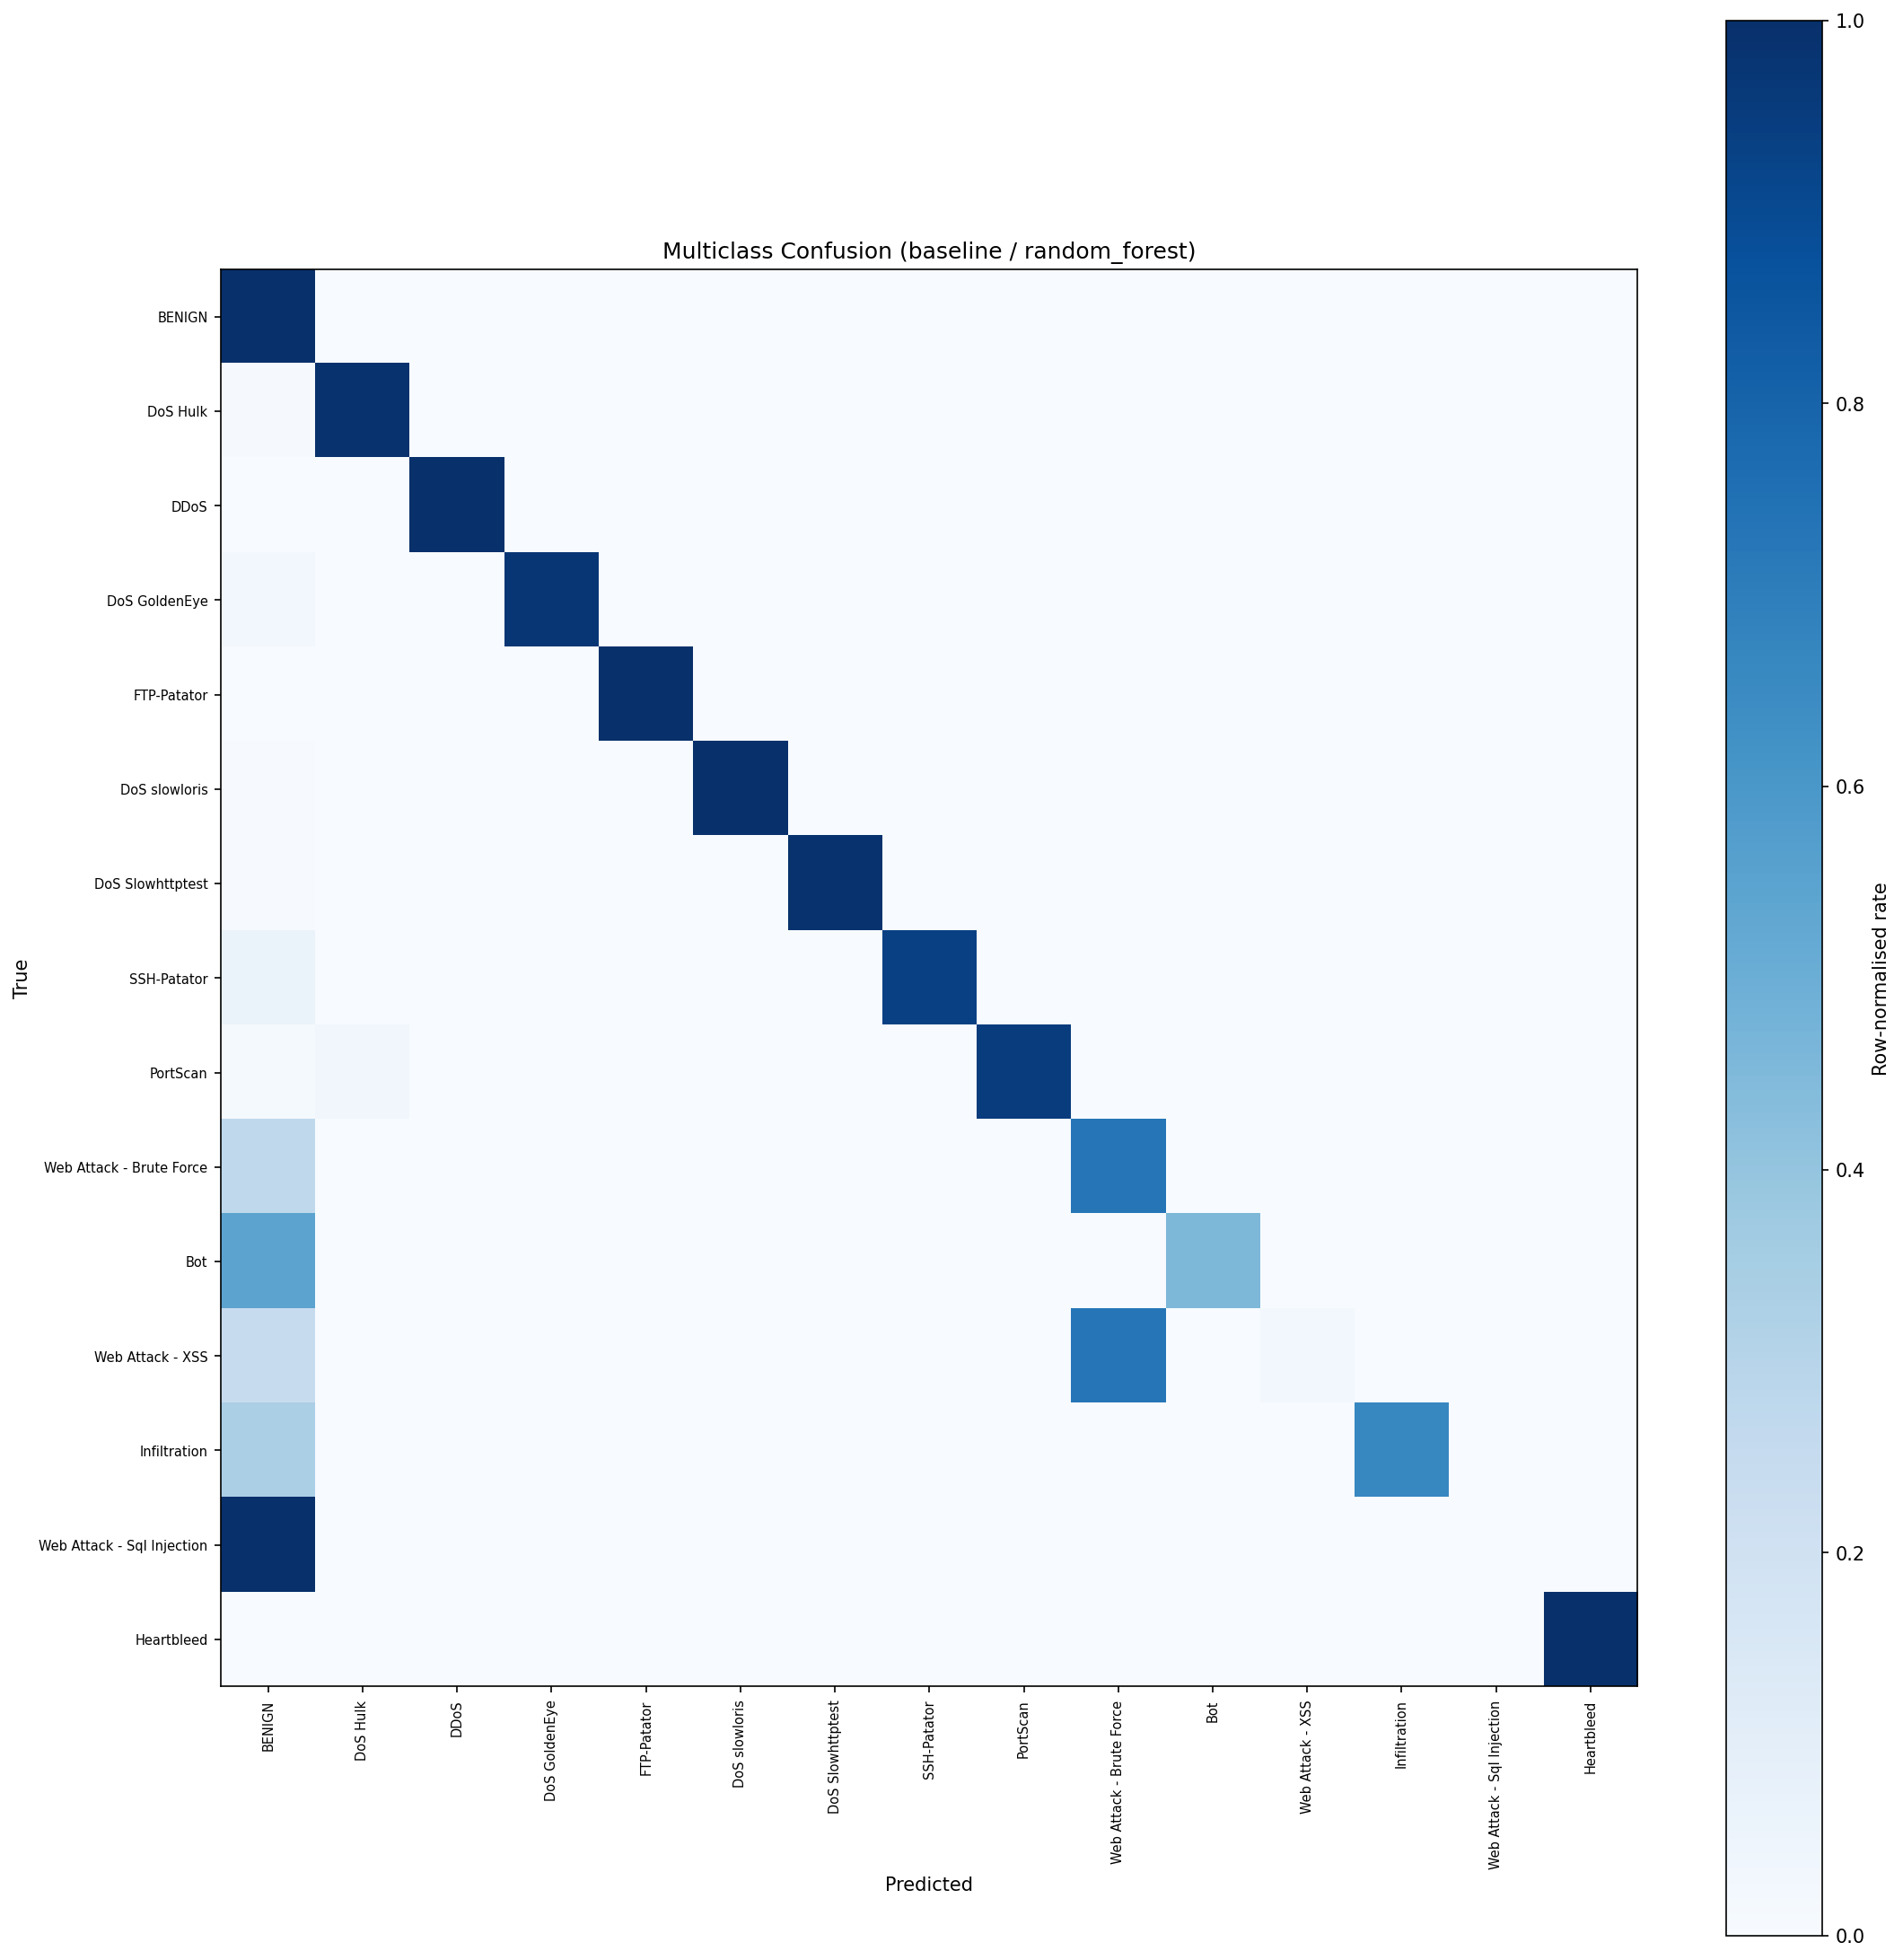
\includegraphics[width=0.7\textwidth]{img/confusion_matrix.png}}{\fbox{\parbox{0.66\textwidth}{\centering\vspace{1.4cm}\ph{Ma trận nhầm lẫn đa lớp --- chạy ml\_09\_multiclass\_eval.py}\vspace{1.4cm}}}}
    \caption{Ma trận nhầm lẫn đa lớp theo loại tấn công (chuẩn hóa theo hàng)}
    \label{fig:confusion_matrix}
\end{figure}

\textbf{Phân tích hướng nhầm lẫn giữa các lớp hiếm.} Đọc ma trận nhầm lẫn theo \emph{đích đến} của các dự đoán sai cho thấy các lớp hiếm suy giảm theo hai kiểu khác nhau. Kiểu thứ nhất là \emph{nhầm loại nhưng vẫn bị phát hiện}: 81/111 mẫu Web Attack~--~XSS bị gán thành Web Attack~--~Brute Force, tức ở bài toán nhị phân triển khai trên biên, các luồng này \emph{vẫn bị gắn cờ tấn công} (76\% XSS vẫn bị chặn), chỉ sai ở khâu định danh loại. Kiểu thứ hai nguy hiểm hơn: \emph{lọt hẳn thành Benign}: toàn bộ 6/6 mẫu SQL Injection, 158/290 mẫu Bot (54\%) và 84/311 mẫu Web Brute Force bị dự đoán là lưu lượng bình thường. Ba cơ chế giải thích hiện tượng này: (i)~\emph{mất cân bằng cực đoan} (6--311 mẫu so với 380.119 mẫu Benign) khiến các lớp hiếm gần như không có vùng quyết định riêng; (ii)~việc \emph{loại \texttt{destination\_port}} ảnh hưởng nặng nhất đến nhóm tấn công web: khi mất ``lối tắt'' cổng 80, các luồng HTTP tấn công (request/response ngắn) có đặc trưng hành vi rất gần lưu lượng duyệt web thường và gần lẫn nhau; giá trị recall 0{,}027 của XSS là con số \emph{trung thực} thay cho con số đẹp nhờ rò rỉ; (iii)~\emph{Bot lẫn Benign do bản chất}: các luồng beaconing C\&C nhỏ, đều đặn, giống lưu lượng nền khi không còn định danh cổng/dịch vụ. Nhận diện này định hướng trực tiếp cho hướng phát triển: xử lý mất cân bằng có chủ đích (tăng cường/oversampling lớp hiếm), bổ sung đặc trưng chuỗi thời gian cho hành vi beaconing, và kiểm chứng liên bộ dữ liệu (Mục~\ref{sec:cross-dataset}).

\pagebreak

\clearpage
\section{Thực nghiệm và đánh giá hiệu năng mô hình trên Jetson Orin Nano Super}

Trong phần này, luận văn đề xuất xây dựng một hệ thống phát hiện xâm nhập mạng \ac{ids} \emph{phân tán} triển khai trên một cụm \textbf{hai thiết bị biên NVIDIA Jetson Orin Nano Super}~\cite{nvidia2019jetson} nhằm đánh giá khả năng hoạt động trong môi trường tài nguyên hạn chế; đây là hướng tiếp cận điện toán biên đưa phân tích về gần nguồn dữ liệu để giảm băng thông và thời gian phản hồi \cite{shi2016edge,hamdan2020edge}, trong khi các nghiên cứu IDS biên trước đây chủ yếu đánh giá suy luận đơn nút \cite{sforzin2016rpids}. Hệ thống được thiết kế theo kiến trúc xử lý dữ liệu thời gian thực hai tầng: một \emph{cổng phát hiện bất thường} (anomaly gate) bằng autoencoder nhẹ lọc bớt lưu lượng bình thường trên Jetson~\#1, và một \emph{bộ phân loại} PySpark \texttt{PipelineModel} chỉ xử lý các luồng nghi vấn trên Jetson~\#2. Hạ tầng trung tâm (Apache Kafka cho truyền tải thông điệp, PostgreSQL để quản lý dữ liệu, InfluxDB để lưu chỉ số hiệu năng theo thời gian, Grafana để trực quan hóa và Mailtrap để kiểm thử cảnh báo qua email) chạy trên một máy chủ điều phối.

NVIDIA Jetson Orin Nano Super là một máy tính nhúng (single-board computer) tích hợp CPU kiến trúc ARM 64-bit và GPU NVIDIA, hỗ trợ tăng tốc suy luận học máy ngay tại biên; cấu hình chi tiết đã nêu tại Bảng~\ref{tab:hardware} (Chương~3) và mục Môi trường thực nghiệm. Do hạn chế về tài nguyên tính toán so với máy chủ truyền thống, việc triển khai trên Jetson Orin Nano Super cho phép đánh giá khả năng tối ưu hóa mô hình và hiệu năng suy luận trong điều kiện phần cứng nhúng (edge computing).

Mô hình có hiệu năng tối ưu được xác định ở phần đánh giá hiệu năng phân loại phía trên sẽ được tích hợp vào pipeline xử lý nhằm thực hiện nhiệm vụ phát hiện và phân loại lưu lượng mạng thành hai nhóm: \textit{Benign} và \textit{Attack}. Các chỉ số đánh giá bao gồm độ chính xác (Accuracy), Precision, Recall, F1-Score, thời gian dự đoán trung bình cho mỗi mẫu, thông lượng xử lý (throughput) và mức tiêu thụ tài nguyên hệ thống (CPU, RAM). Kết quả thực nghiệm cho phép phân tích tính khả thi của việc triển khai hệ thống \ac{ids} dựa trên học máy trong môi trường thiết bị biên có tài nguyên giới hạn.

\subsection{Các công cụ sử dụng trong hệ thống}

Trong hệ thống phát hiện xâm nhập mạng \ac{ids} được đề xuất, ngoài các công nghệ xử lý dữ liệu lớn đã trình bày ở Chương~2, luận văn sử dụng thêm một số công cụ và nền tảng mã nguồn mở nhằm hỗ trợ truyền tải dữ liệu, lưu trữ, giám sát hiệu năng và cảnh báo theo thời gian thực. Cụ thể:

\begin{itemize}

    \item \textbf{Apache Kafka}~\cite{Kreps2011} -- Là nền tảng truyền tải thông điệp phân tán (distributed event streaming platform), được sử dụng để tiếp nhận và phân phối dữ liệu luồng theo cơ chế publish-subscribe. Trong hệ thống, Kafka đóng vai trò trung gian giữa nguồn dữ liệu (CICIDS2017 được mô phỏng bằng Python script) và thiết bị Jetson Orin Nano Super, đảm bảo khả năng truyền tải bất đồng bộ, chịu lỗi và mở rộng linh hoạt.

    \item \textbf{Apache Spark Streaming} -- Là thành phần xử lý dữ liệu luồng thời gian thực. Spark Streaming nhận dữ liệu từ Kafka Consumer, thực hiện các bước tiền xử lý đặc trưng và chuyển dữ liệu đến mô hình học máy đã được huấn luyện để thực hiện suy luận.

    \item \textbf{PostgreSQL} -- Là hệ quản trị cơ sở dữ liệu quan hệ mã nguồn mở có độ ổn định và khả năng mở rộng cao. Trong hệ thống, PostgreSQL được sử dụng để lưu trữ kết quả dự đoán, thông tin cảnh báo và các bản ghi phục vụ báo cáo tổng hợp.

    \item \textbf{InfluxDB} -- Là cơ sở dữ liệu chuỗi thời gian (Time-Series Database), tối ưu cho việc lưu trữ và truy vấn các chỉ số theo thời gian. Hệ thống sử dụng InfluxDB để ghi nhận các thông số hiệu năng như thời gian suy luận, mức sử dụng CPU, bộ nhớ và thông lượng xử lý.

    \item \textbf{Grafana} -- Là nền tảng trực quan hóa dữ liệu mã nguồn mở, cho phép xây dựng các dashboard theo thời gian thực. Grafana kết nối với InfluxDB và PostgreSQL để hiển thị tình trạng hoạt động của hệ thống \ac{ids} cũng như thống kê các sự kiện tấn công.

    \item \textbf{Mailtrap} -- Là công cụ kiểm thử email trong môi trường giả lập. Trong giai đoạn thực nghiệm, Mailtrap được sử dụng để kiểm tra cơ chế gửi cảnh báo khi hệ thống phát hiện lưu lượng mạng bất thường trước khi triển khai môi trường thực tế.

\end{itemize}

Việc tích hợp các công nghệ trên giúp hệ thống đảm bảo khả năng xử lý dữ liệu thời gian thực, lưu trữ an toàn, giám sát hiệu năng liên tục và kích hoạt cảnh báo kịp thời khi phát hiện hành vi xâm nhập.

\pagebreak
\subsection{Mô hình hệ thống đề xuất}
Hệ thống phát hiện xâm nhập được thiết kế theo kiến trúc xử lý dữ liệu luồng như minh họa ở Hình~\ref{fig:ids_diagram}. Luồng xử lý tổng thể bao gồm các bước sau:
\begin{figure}[ht]
    \centering
    \resizebox{\textwidth}{!}{%
    \begin{tikzpicture}[
        font=\small, >=Stealth,
        every node/.style={align=center},
        pc/.style ={draw=gray!60,         thick, rounded corners, fill=gray!8,  minimum width=13.4cm, minimum height=1.3cm, inner sep=3pt},
        jet/.style={draw=accGreen!80!black,  thick, rounded corners, fill=accGreen!8, text width=4.2cm, minimum height=2.0cm, inner sep=4pt},
        mtr/.style={draw=accBlue,         thick, rounded corners, fill=accBlue!5,  minimum width=13.4cm, minimum height=1.0cm, inner sep=3pt},
        lbl/.style={font=\footnotesize, fill=white, inner sep=1.5pt, align=center, text=accBlue!75!black},
        arr/.style ={-{Stealth[length=2.5mm]}, thick, draw=gray!60!black},
        dsh/.style={-{Stealth[length=2.5mm]}, thick, draw=accBlue, dashed},
    ]
        \node[pc]  (pc)  at (0, 0.0)   {\textbf{Máy chủ điều phối (MacBook, Docker)}\\[2pt]
            Apache Kafka \;$|$\; PostgreSQL \;$|$\; InfluxDB \;$|$\; Grafana \;$|$\; \texttt{data\_sender.py}};
        \node[jet] (j1)  at (-4.6,-4.7) {\textbf{Jetson Orin Nano Super \#1}\\[2pt] \texttt{anomaly\_gate}\\[2pt]
            Autoencoder lọc bớt\\ lưu lượng bình thường};
        \node[jet] (j2)  at ( 4.6,-4.7) {\textbf{Jetson Orin Nano Super \#2}\\[2pt] \texttt{classifier}\\[2pt]
            PySpark \texttt{PipelineModel}\\ phân loại Benign / Attack};
        \node[mtr] (out) at (0,-9.0)    {Chỉ số hiệu năng $\rightarrow$ InfluxDB $\rightarrow$ Grafana \quad$|$\quad
            Cảnh báo: Email (Mailtrap) / Slack};

        \draw[arr] (pc.south -| j1) -- node[lbl]{topic\\ \texttt{ids-network-flow}} (j1.north);
        \draw[arr] (j1.east) -- node[lbl]{\texttt{ids-suspicious-flow}\\ (luồng nghi vấn)} (j2.west);
        \draw[arr] (j2.north) -- node[lbl]{kết quả phân loại\\ $\rightarrow$ PostgreSQL} (pc.south -| j2);
        % Mũi tên gạch đứt (metric/cảnh báo) đi thẳng vào CẠNH TRÊN của dải, không cắt chữ.
        \draw[dsh] (j1.south) -- (out.north -| j1);
        \draw[dsh] (j2.south) -- (out.north -| j2);
    \end{tikzpicture}%
    }
    \caption[Kiến trúc hệ thống IDS phân tán trên cụm 2 Jetson Orin Nano Super]{Kiến trúc hệ thống phát hiện xâm nhập phân tán thời gian thực trên cụm 2 Jetson Orin Nano Super}
    \label{fig:ids_diagram}
\end{figure}

\pagebreak
\begin{enumerate}

    \item \textbf{Nguồn dữ liệu}:
    Dữ liệu từ bộ CICIDS2017 được mô phỏng theo thời gian thực thông qua một Python script và gửi vào Kafka Producer trên topic \texttt{ids-network-flow}.

    \item \textbf{Cổng phát hiện bất thường (Jetson~\#1)}:
    Jetson~\#1 đảm nhận vai trò \texttt{anomaly\_gate}: một autoencoder nhẹ (huấn luyện chỉ trên lưu lượng bình thường) tính sai số tái tạo (reconstruction error) cho từng luồng. Các luồng có sai số dưới ngưỡng được coi là bình thường và \emph{được lọc bỏ}; chỉ các luồng \emph{nghi vấn} mới được chuyển tiếp sang topic \texttt{ids-suspicious-flow}. Cơ chế này giảm đáng kể khối lượng phải đưa vào suy luận Spark.

    \item \textbf{Bộ phân loại (Jetson~\#2)}:
    Jetson~\#2 đảm nhận vai trò \texttt{classifier}: tải mô hình PySpark \texttt{PipelineModel} (với tập đặc trưng SHAP Top-30 đã chọn) và phân loại các luồng nghi vấn thành \textit{Benign} hoặc \textit{Attack}. Vector đầu vào khi triển khai gồm 29 đặc trưng: trong Top-30 theo xếp hạng SHAP có \texttt{destination\_port}, nhưng đặc trưng này bị loại khỏi mô hình xuất ra để triển khai vì là kênh rò rỉ nhãn trên CICIDS2017 (Mục~\ref{sec:leakage_analysis}), nhất quán với giao thức chống rò rỉ ở pha huấn luyện.

    \item \textbf{Ghi nhận hiệu năng}:
    Mỗi nút ghi nhận thời gian dự đoán/mẫu, mức sử dụng CPU/RAM/nhiệt độ và thông lượng (gắn nhãn theo \texttt{EDGE\_NODE\_ID}); các chỉ số được lưu vào InfluxDB.

    \item \textbf{Lưu trữ và cảnh báo}:
    Kết quả dự đoán và sự kiện tấn công được lưu vào PostgreSQL; khi phát hiện lưu lượng bất thường, hệ thống kích hoạt cảnh báo qua Email/\allowbreak Webhook (Mailtrap, Slack trong môi trường kiểm thử) từ một nút chính được chỉ định để tránh trùng lặp.

    \item \textbf{Trực quan hóa và giám sát}:
    Grafana truy xuất dữ liệu từ InfluxDB và PostgreSQL để xây dựng dashboard theo thời gian thực, giám sát trạng thái hệ thống và thống kê các sự kiện tấn công.

\end{enumerate}

\textbf{Ba chế độ triển khai phân tán.} Cụm hai Jetson hỗ trợ ba chế độ, lựa chọn theo ràng buộc tải và độ trễ:
\begin{itemize}
    \item \textbf{Chế độ A -- Pipeline split} (khuyến nghị): Jetson~\#1 = cổng bất thường (anomaly gate), Jetson~\#2 = bộ phân loại (classifier) (như mô tả trên), giúp giảm tải Spark nhờ lọc lưu lượng bình thường sớm.
    \item \textbf{Chế độ B -- Mở rộng theo chiều ngang (Horizontal scaling)}: cả hai Jetson chạy pipeline đầy đủ trong cùng một nhóm tiêu thụ (consumer group) của Kafka nhằm tăng thông lượng.
    \item \textbf{Chế độ C -- Spark cluster}: máy chủ MacBook làm Spark master, hai Jetson làm worker, phân tán suy luận Spark trên cụm. Nhất quán với nguyên tắc ở mục Môi trường thực nghiệm, MacBook chỉ đảm nhận điều phối (master), không chạy executor; toàn bộ tính toán suy luận vẫn nằm trên hai Jetson.
\end{itemize}

Kiến trúc này đảm bảo tính mô-đun, tách biệt các thành phần xử lý, đồng thời phù hợp với mô hình triển khai phân tán trên các thiết bị biên có tài nguyên hạn chế như Jetson Orin Nano Super.

\textbf{Đặc tả cổng bất thường (operating point).} Cổng autoencoder là một bộ lọc \emph{điều chỉnh được} chứ không phải một điểm cố định: nâng ngưỡng giúp giảm tải (offload) nhiều lưu lượng bình thường hơn khỏi Spark (tăng tỷ lệ bỏ qua tại cổng, gate-skip) nhưng có thể giảm recall trên lớp tấn công. Ngưỡng của cổng được chọn theo phân vị (quantile) của sai số tái tạo tính trên một \emph{tập kiểm định benign}, gồm 10\% tách từ phần lưu lượng bình thường của tập huấn luyện (\texttt{seed}=42); tập kiểm tra không tham gia việc chọn ngưỡng, tránh rò rỉ kiểu ``ngưỡng oracle''. Bảng~\ref{tab:gate_oc} trình bày đường đánh đổi giữa recall và mức giảm tải (recall--offload) khi quét các mức quantile trên tập kiểm định này; điểm vận hành được chọn theo ngân sách độ trễ/độ chính xác của triển khai. FPR trong bảng là tỷ lệ luồng benign bị cổng chuyển nhầm sang bộ phân loại, không phải FPR của toàn hệ thống.

\begin{table}[htbp]
\centering
\caption[Điểm vận hành của cổng bất thường theo ngưỡng quantile]{Điểm vận hành của cổng bất thường theo ngưỡng quantile trên tập kiểm định benign}
\label{tab:gate_oc}
\begin{tabular*}{\textwidth}{@{\extracolsep{\fill}}ccccc@{}}
\toprule
\textbf{Quantile (validation)} & \textbf{Ngưỡng} & \textbf{Recall (Attack)} & \textbf{FPR} & \textbf{Tỷ lệ bỏ qua tại cổng (\%)} \\ \midrule
0{,}90 & 0{,}0023 & 0{,}7589 & 0{,}1003 & 80{,}08 \\
0{,}95 & 0{,}0052 & 0{,}7552 & 0{,}0506 & 84{,}36 \\
0{,}99 & 0{,}0192 & 0{,}7420 & 0{,}0101 & 88{,}00 \\
0{,}995 & 0{,}0317 & 0{,}7229 & 0{,}0053 & 88{,}70 \\ \bottomrule
\end{tabular*}
\end{table}


\subsection{Lựa chọn mô hình cho thiết bị biên}

Triển khai trên thiết bị biên đặt ra các ràng buộc về tài nguyên: RAM 8\,GB chia sẻ giữa CPU và GPU (trong đó PySpark JVM chiếm một phần đáng kể), CPU ARM, cùng ràng buộc về nhiệt độ/băng thông tại biên. Cũng cần nhấn mạnh rằng việc chọn Apache Spark trên Jetson 8\,GB phải chịu chi phí JVM/Spark đáng kể; Spark được dùng ở đây nhằm \emph{nhất quán} với pha huấn luyện phân tán, chứ không nhằm tối ưu độ trễ suy luận trên một nút; chi phí đánh đổi này được định lượng qua so sánh với scikit-learn và ONNX Runtime ở mục~\ref{sec:engine-baseline-thesis}, còn tăng tốc bằng TensorRT là hướng nghiên cứu tương lai. Ba mô hình đại diện cho ba thử nghiệm khác nhau được chọn để đánh giá:

\begin{enumerate}
    \item \textbf{Decision Tree} -- Mô hình cây đơn lẻ, đại diện cho cách tiếp cận đơn giản nhất.
    \item \textbf{\ac{gbt} (Gradient-Boosted Trees)} -- Đại diện cho phương pháp Boosting, sử dụng nhiều cây yếu kết hợp tuần tự.
    \item \textbf{Random Forest} -- Đại diện cho phương pháp Bagging, sử dụng ensemble 200 cây song song.
\end{enumerate}

Cả ba mô hình đều được huấn luyện trên tập SHAP Top-30 đặc trưng và triển khai dưới dạng PySpark PipelineModel.

% LƯU Ý: terminal + Grafana đã chụp lại từ cụm Jetson (2026-07-19). Riêng 2 ảnh
% cảnh báo email/Slack dùng lại ảnh giai đoạn thử nghiệm sớm — chính văn dưới cụm
% hình đã ghi chú tường minh; mô-đun cảnh báo không đổi giữa hai giai đoạn.
\begin{figure}[htbp]
    \centering
    \IfFileExists{img/pipeline_terminal_jetson1.png}{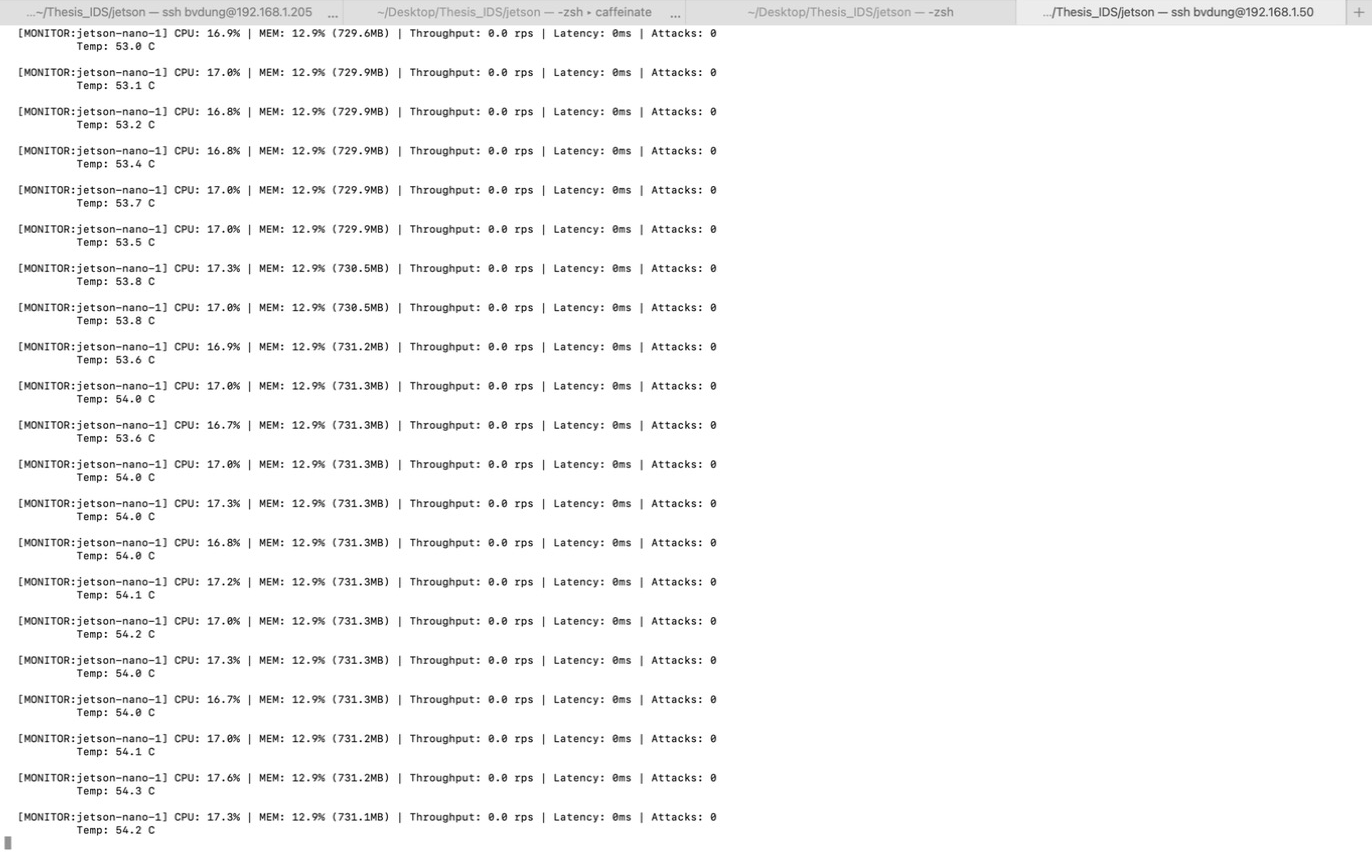
\includegraphics[width=0.85\textwidth]{img/pipeline_terminal_jetson1.png}}{\fbox{\parbox{0.85\textwidth}{\centering\vspace{1.2cm}\ph{Ảnh terminal node cổng (jetson-nano-1)}\vspace{1.2cm}}}}\\[2pt]
    {\footnotesize (a) Jetson \#1 (\texttt{jetson-nano-1}): cổng phát hiện bất thường, giám sát tài nguyên theo node}\\[8pt]
    \IfFileExists{img/pipeline_terminal_jetson2.png}{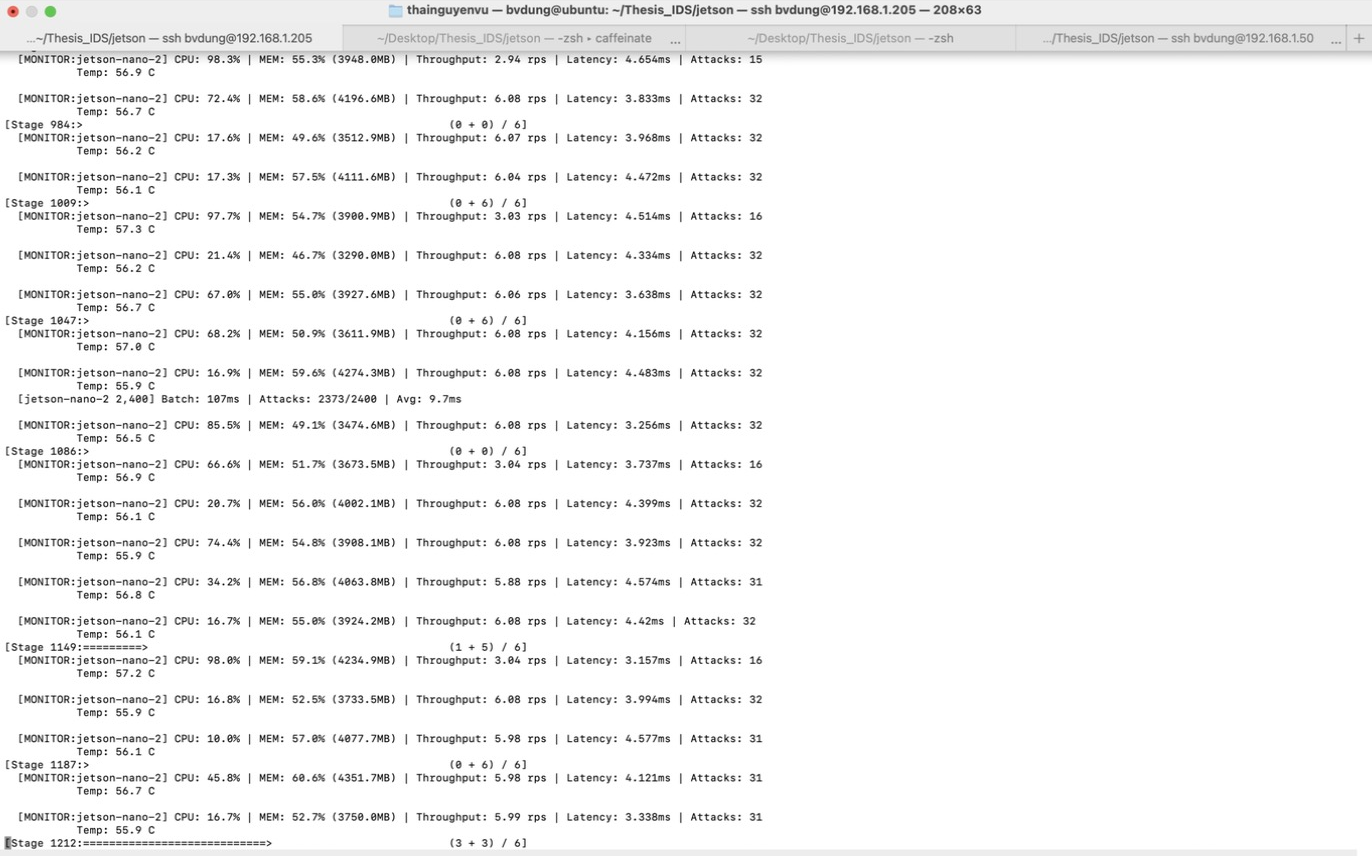
\includegraphics[width=0.85\textwidth]{img/pipeline_terminal_jetson2.png}}{\fbox{\parbox{0.85\textwidth}{\centering\vspace{1.2cm}\ph{Ảnh terminal node phân loại (jetson-nano-2)}\vspace{1.2cm}}}}\\[2pt]
    {\footnotesize (b) Jetson \#2 (\texttt{jetson-nano-2}): bộ phân loại PySpark, thông lượng \textasciitilde6 luồng/giây, độ trễ suy luận \textasciitilde4\,ms, đếm tấn công theo lô}
    \caption[Giao diện terminal của pipeline IDS trên hai node Jetson]{Giao diện terminal của pipeline IDS trên hai node Jetson: (a) cổng lọc bất thường, (b) bộ phân loại PySpark}
    \label{fig:pipeline_terminal}
\end{figure}

\begin{figure}[htbp]
    \centering
    \IfFileExists{img/grafana_dashboard.png}{
\includegraphics[width=0.9\textwidth]{img/grafana_dashboard.png}}{\fbox{\parbox{0.85\textwidth}{\centering\vspace{1.2cm}\ph{Dashboard Grafana hiệu năng --- chụp lại từ cụm Jetson}\vspace{1.2cm}}}}
    \caption{Dashboard Grafana giám sát hiệu năng IDS theo thời gian thực}
    \label{fig:grafana_dashboard}
\end{figure}


\begin{figure}[htbp]
    \centering
    \IfFileExists{img/mailtrap_alert.png}{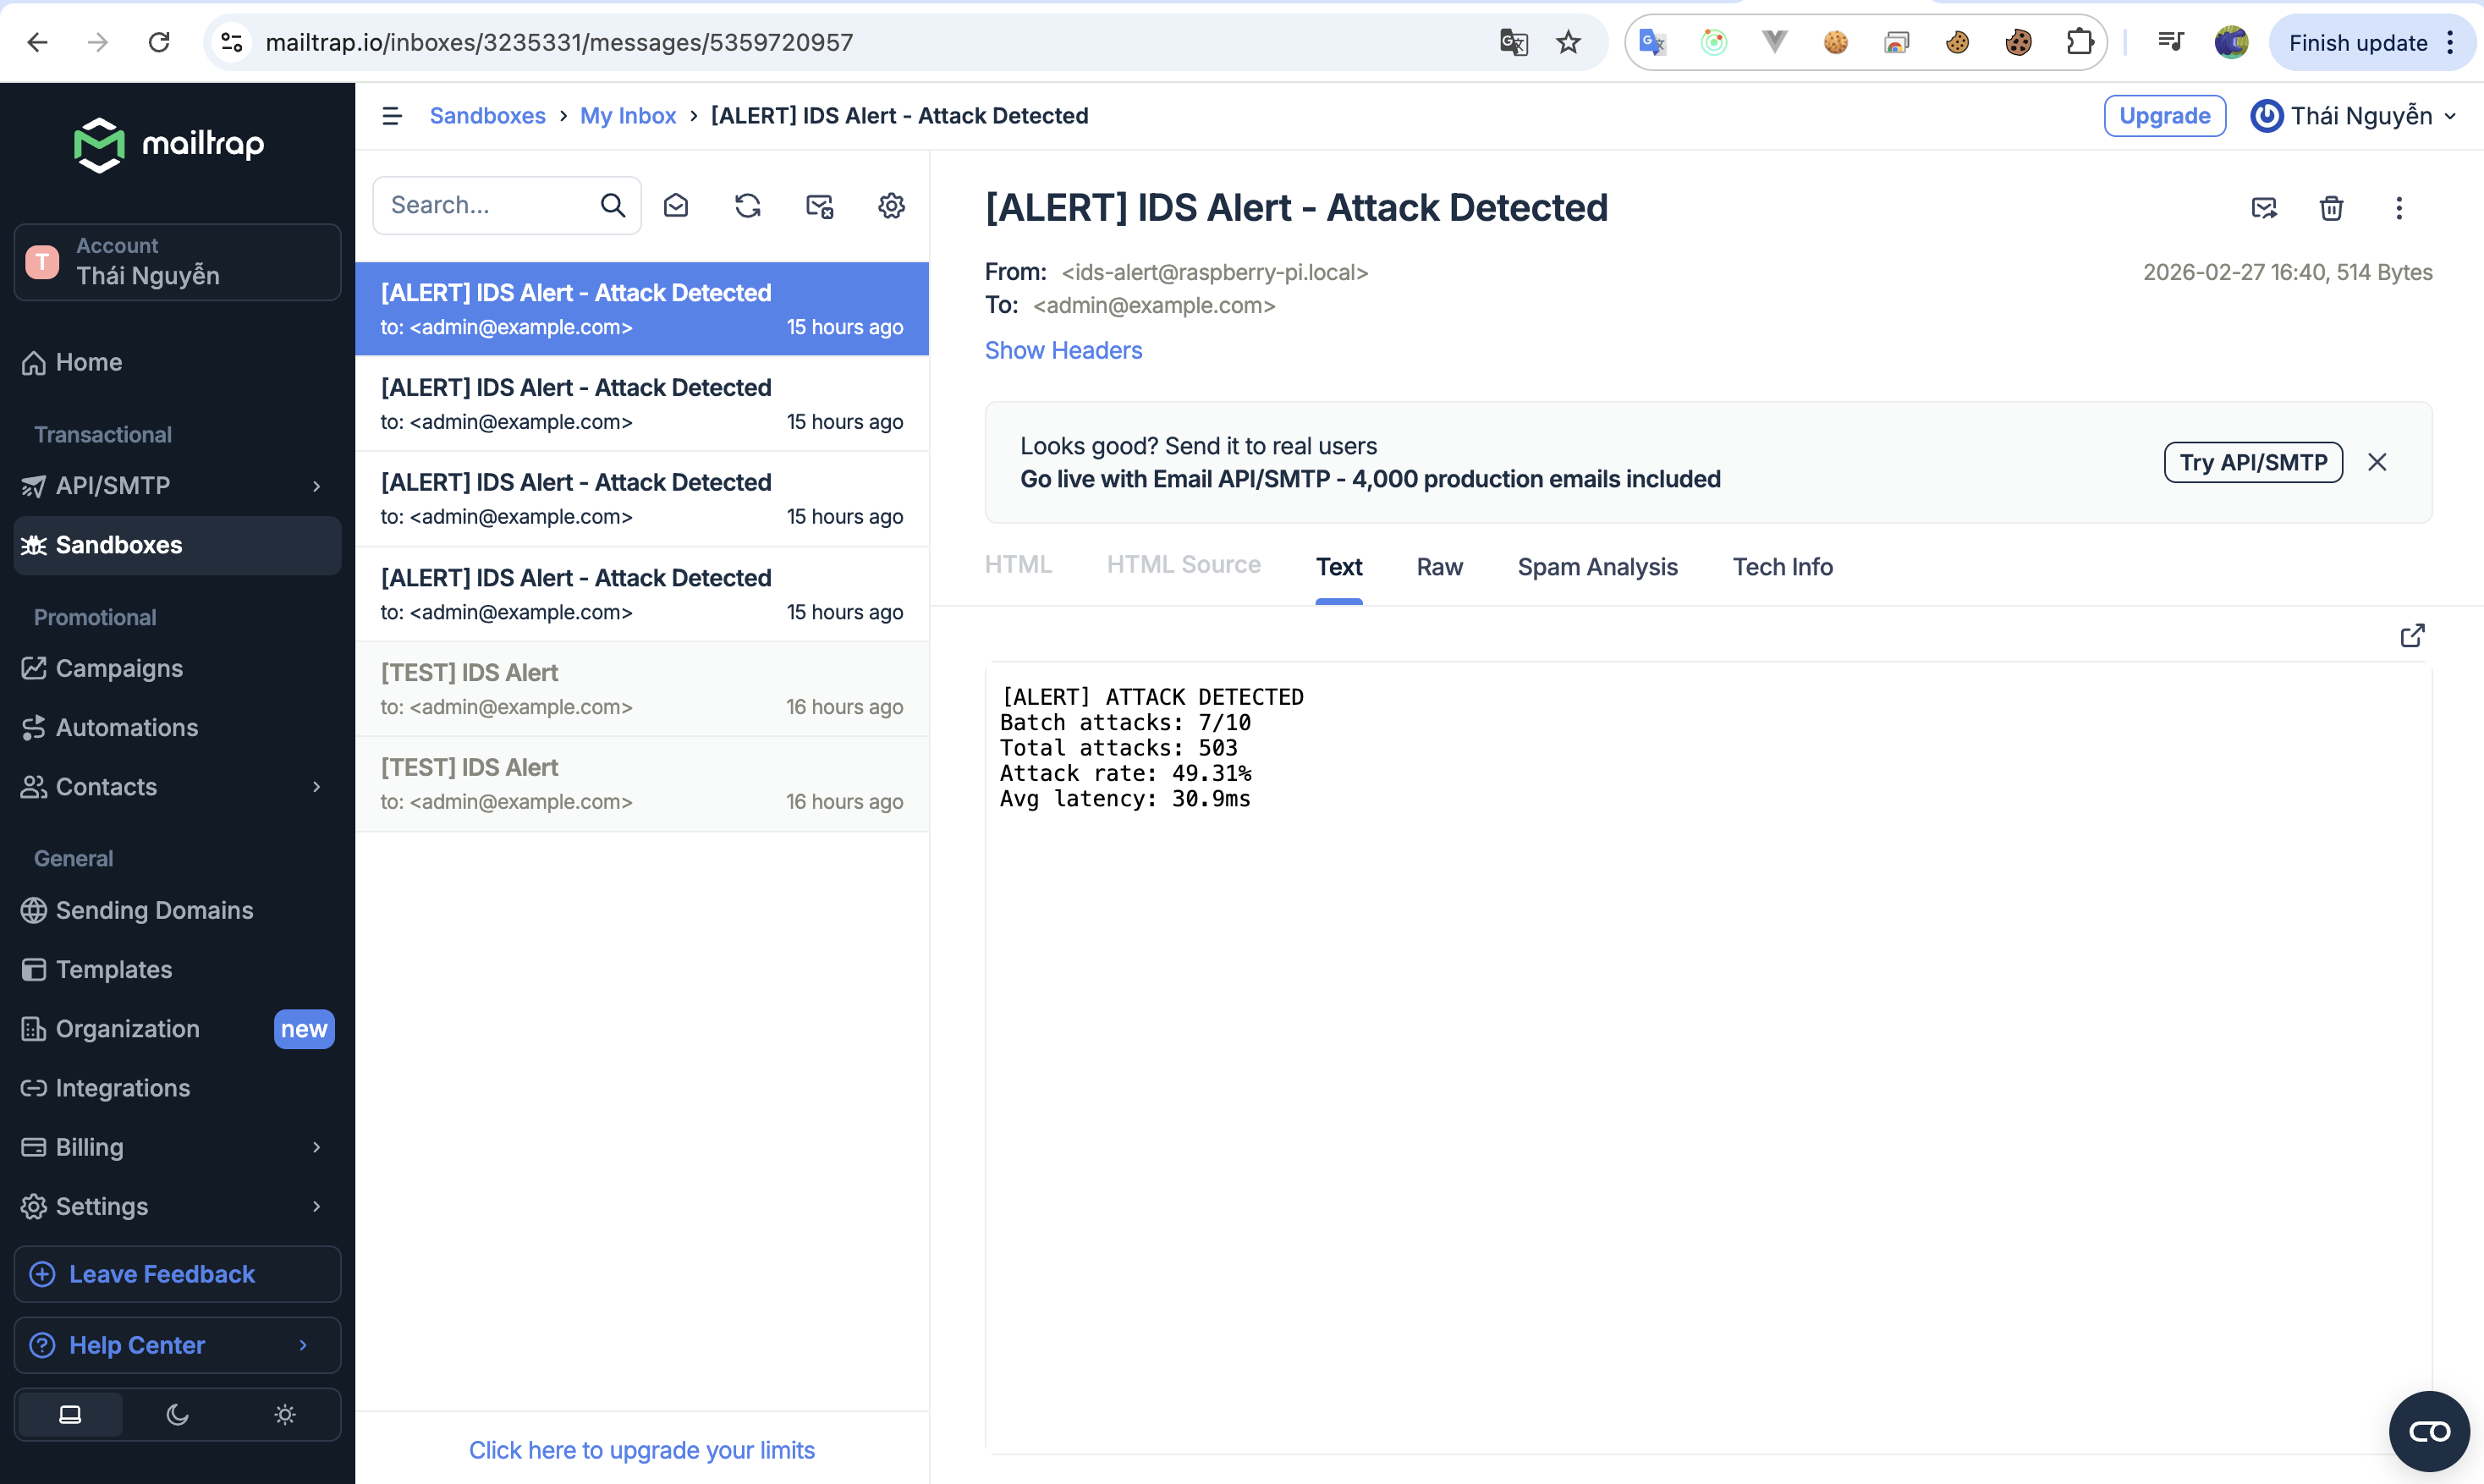
\includegraphics[width=0.9\textwidth]{img/mailtrap_alert.png}}{\fbox{\parbox{0.85\textwidth}{\centering\vspace{1.2cm}\ph{Email cảnh báo Mailtrap --- chụp lại từ hệ chạy trên Jetson}\vspace{1.2cm}}}}
    \caption[Email cảnh báo tấn công gửi qua Mailtrap]{Email cảnh báo tấn công gửi qua Mailtrap trong môi trường kiểm thử}
    \label{fig:mailtrap_alert}
\end{figure}

\begin{figure}[htbp]
    \centering
    \IfFileExists{img/grafana_attacks.png}{
\includegraphics[width=0.9\textwidth]{img/grafana_attacks.png}}{\fbox{\parbox{0.85\textwidth}{\centering\vspace{1.2cm}\ph{Dashboard Grafana chi tiết tấn công --- chụp lại từ cụm Jetson}\vspace{1.2cm}}}}
    \caption[Dashboard Grafana chi tiết các cuộc tấn công được phát hiện]{Dashboard Grafana hiển thị chi tiết các cuộc tấn công được phát hiện và phân loại theo thời gian}
    \label{fig:grafana_attacks}
\end{figure}

\begin{figure}[htbp]
    \centering
    \IfFileExists{img/grafana_peak_load.png}{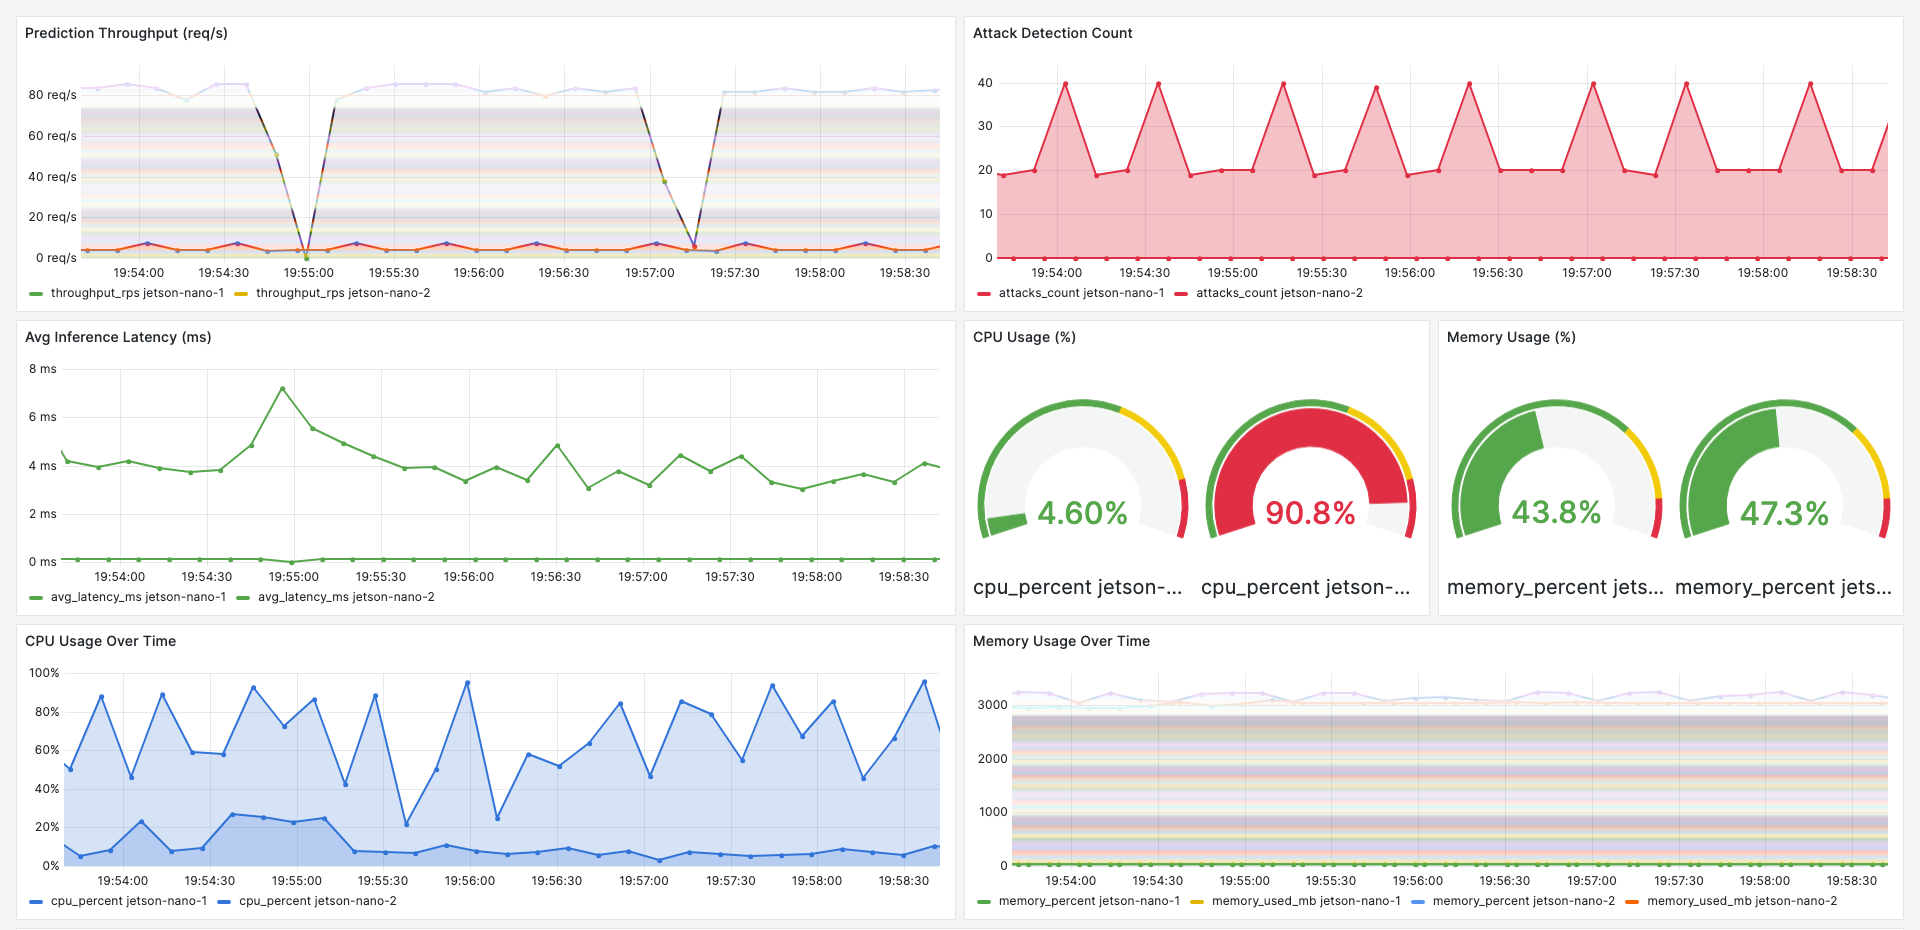
\includegraphics[width=0.9\textwidth]{img/grafana_peak_load.png}}{\fbox{\parbox{0.85\textwidth}{\centering\vspace{1.2cm}\ph{Dashboard Grafana tại thời điểm tải đỉnh --- chụp lại từ cụm Jetson}\vspace{1.2cm}}}}
    \caption[Dashboard Grafana tại thời điểm tải đỉnh của chế độ tách pipeline]{Dashboard Grafana tại thời điểm tải đỉnh của chế độ tách pipeline}
    \label{fig:grafana_peak_load}
\end{figure}

\begin{figure}[htbp]
    \centering
    \IfFileExists{img/slack_alert.png}{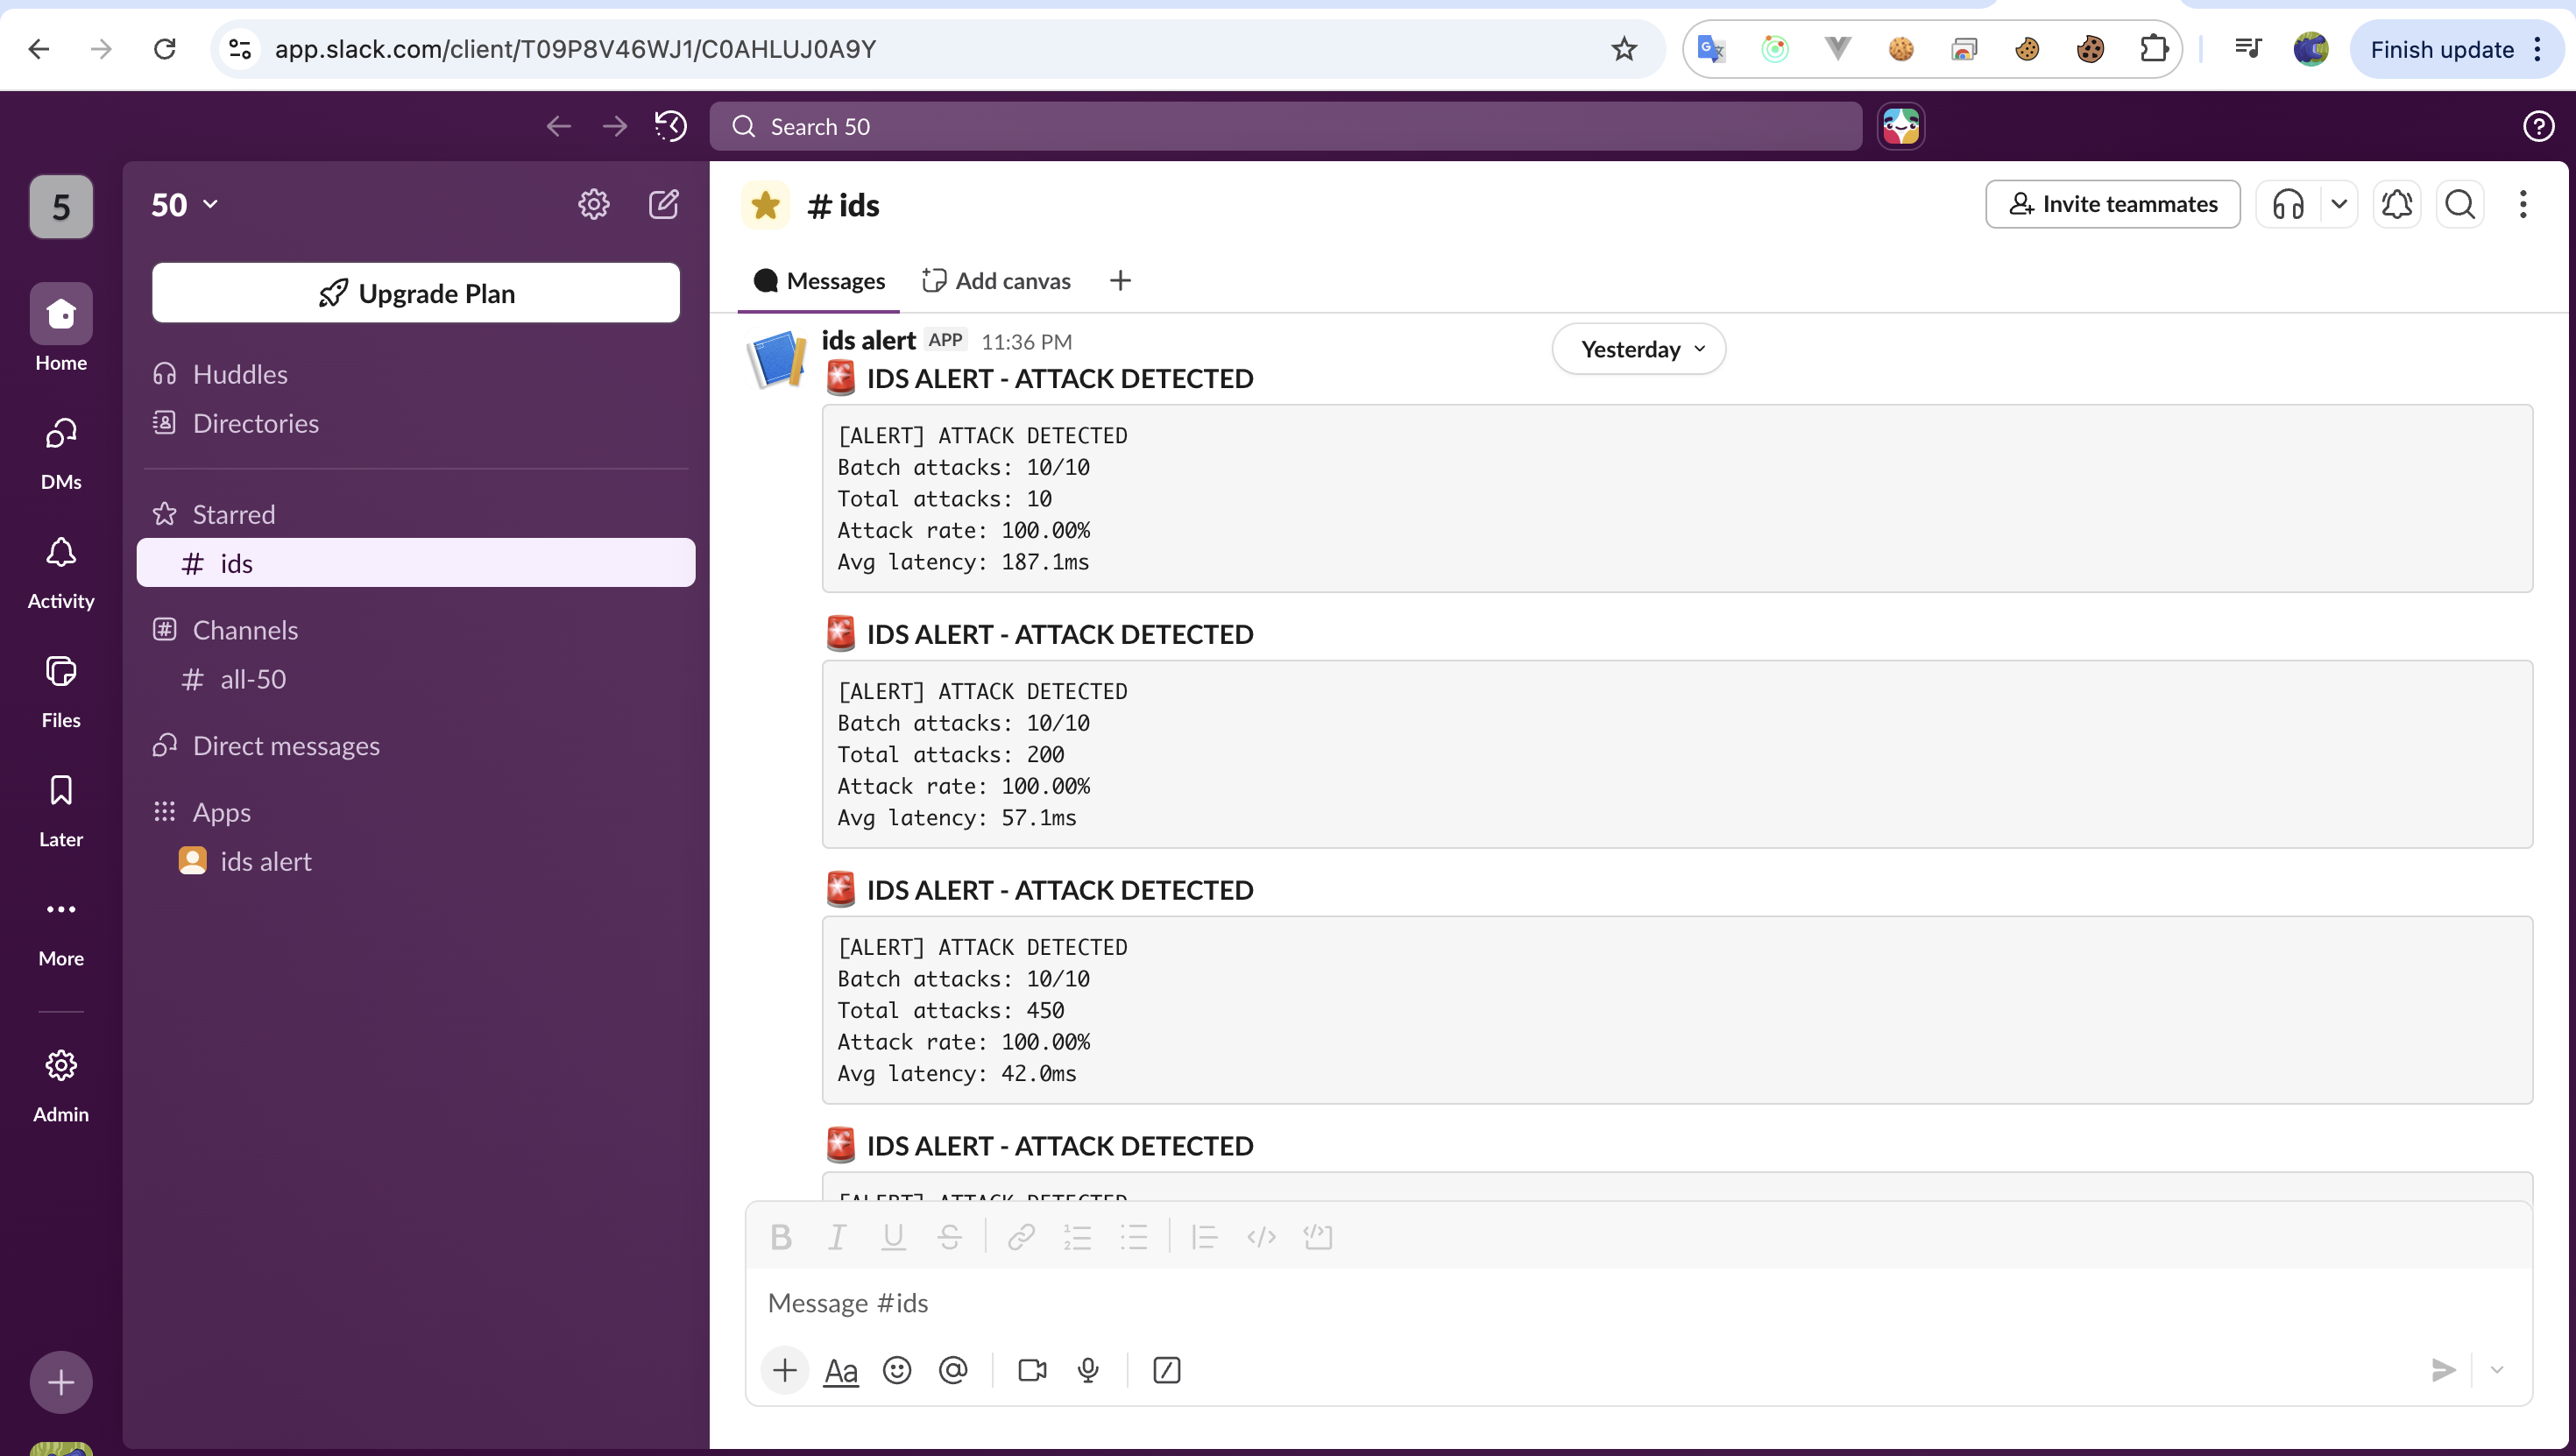
\includegraphics[width=0.9\textwidth]{img/slack_alert.png}}{\fbox{\parbox{0.85\textwidth}{\centering\vspace{1.2cm}\ph{Thông báo Slack --- chụp lại từ hệ chạy trên Jetson}\vspace{1.2cm}}}}
    \caption[Thông báo cảnh báo tấn công gửi qua Slack]{Thông báo cảnh báo tấn công gửi qua Slack Incoming Webhook}
    \label{fig:slack_alert}
\end{figure}

Hình~\ref{fig:pipeline_terminal} minh họa giao diện terminal thực tế khi pipeline IDS đang xử lý dữ liệu trên Jetson Orin Nano Super, bao gồm thông tin về thông lượng, độ trễ và số lượng tấn công phát hiện được. Hai dashboard Grafana (Hình~\ref{fig:grafana_dashboard} và Hình~\ref{fig:grafana_attacks}) cho phép giám sát hiệu năng hệ thống và chi tiết các cuộc tấn công theo thời gian thực. Hình~\ref{fig:grafana_peak_load} ghi lại thời điểm tải đỉnh, cho thấy rõ sự phân bố tải lệch đặc trưng của chế độ tách pipeline: nút cổng chỉ sử dụng khoảng 5\,\% CPU trong khi nút phân loại PySpark đạt tới 91\,\%, xác nhận bộ phân loại là thành phần chiếm tài nguyên chủ đạo và là căn cứ cho các phân tích năng lượng--thông lượng ở phần sau. Khi phát hiện tấn công, hệ thống tự động gửi cảnh báo qua nhiều kênh: email thông qua Mailtrap SMTP (Hình~\ref{fig:mailtrap_alert}) và tin nhắn Slack (Hình~\ref{fig:slack_alert}). Hai ảnh cảnh báo này chụp từ giai đoạn thử nghiệm sớm của hệ thống; mô-đun cảnh báo và định dạng thông điệp giữ nguyên khi triển khai trên cụm Jetson.
\subsection{Kết quả huấn luyện các mô hình ứng viên trên cụm Spark}

Bảng \ref{tab:edge_training} trình bày kết quả huấn luyện và đánh giá ba mô hình ứng viên trên cụm Spark (mô tả ở mục Môi trường thực nghiệm) trước khi triển khai xuống thiết bị biên.

\begin{table}[htbp]
\centering
\caption[Các mô hình ứng viên cho triển khai biên (SHAP Top-30)]{Kết quả huấn luyện các mô hình ứng viên cho triển khai biên (SHAP Top-30)}
\label{tab:edge_training}
\begin{tabular*}{\textwidth}{@{\extracolsep{\fill}}lcccc@{}}
\toprule
\textbf{Mô hình} & \textbf{F1-Score} & \textbf{Accuracy} & \textbf{Thời gian huấn luyện (s)} & \textbf{Kích thước (MB)} \\ \midrule
Decision Tree    & 0{,}9814 & 0{,}9943 & 24{,}4  & 0{,}046 \\
\ac{gbt}              & 0{,}9753 & 0{,}9925 & 341{,}8 & 0{,}865 \\
Random Forest    & 0{,}9826 & 0{,}9947 & 687{,}3 & 4{,}427 \\
\bottomrule
\end{tabular*}
\end{table}

Về tiêu chí \emph{nhận biết ràng buộc biên} (edge-aware), ba mô hình ứng viên đánh đổi khác nhau: Decision Tree có kích thước nhỏ nhất (0,046\,MB, nhỏ hơn Random Forest khoảng 96 lần) và huấn luyện nhanh hơn khoảng 28 lần, trong khi Random Forest đạt F1 cao nhất. Riêng F1/Accuracy chưa đủ để kết luận: quyết định cuối cùng dựa trên số đo vận hành thực tế trên thiết bị (thông lượng, độ trễ, CPU, RAM) ở mục tiếp theo. (Các mô hình ứng viên biên được huấn luyện trên mẫu con phân tầng khi xuất để vừa bộ nhớ một nút, nên F1 thấp hơn chút ít so với kết quả huấn luyện phân tán đầy đủ ở Bảng~\ref{tab:summary_comparison}; độ chính xác chính thức lấy từ pha huấn luyện đầy đủ.)


\subsection{Kết quả đo hiệu năng (benchmark) trên Jetson Orin Nano Super}

Bảng \ref{tab:edge_benchmark} trình bày kết quả đo hiệu năng (benchmark) thực tế trên Jetson Orin Nano Super. Mỗi cấu hình được đo lặp lại 5 lần; trước mỗi cửa sổ đo có giai đoạn khởi động (warm-up) bằng chính lưu lượng thật để làm nóng JVM/JIT, và dữ liệu warm-up bị loại khỏi cửa sổ đo; kết quả báo cáo là trung bình $\pm$ độ lệch chuẩn qua các lần chạy. Hai loại độ trễ được ghi nhận: (i) \emph{độ trễ suy luận} (tiền xử lý + dự đoán) trên từng nút, và (ii) \emph{độ trễ đầu cuối} (từ thời điểm producer gửi đến khi có phán quyết) tính từ nhãn thời gian của producer; giá trị tuyệt đối của loại (ii) chỉ có ý nghĩa khi các máy đồng bộ đồng hồ NTP. Các phân vị độ trễ (p50/p95/p99) được tính ở mức từng lần chạy từ \emph{log thô theo từng luồng} trong đúng cửa sổ tải; với cụm nhiều nút, p95 báo cáo là p95 của nút xấu nhất (không lấy phân vị của các giá trị trung bình theo nút).

\begin{table}[htbp]
\centering
\caption{So sánh hiệu năng triển khai trên Jetson Orin Nano Super}
\label{tab:edge_benchmark}
\small
\begin{tabular*}{\textwidth}{@{\extracolsep{\fill}}lccccc@{}}
\toprule
\textbf{Mô hình} & \textbf{Thông lượng} & \textbf{Độ trễ suy luận (ms)} & \textbf{CPU} & \textbf{RAM} & \textbf{Kích thước} \\
                  & \textbf{(mẫu/giây)} & \textbf{p50 / p95 / p99} & \textbf{(\%)} & \textbf{(\%)} & \textbf{(MB)} \\ \midrule
Decision Tree     & 22{,}0 & 441 / 537 / -- & 46{,}4 & 21{,}9 & 0{,}046 \\
\ac{gbt}               & 24{,}3 & 414 / 439 / -- & 40{,}9 & 24{,}0 & 0{,}865 \\
Random Forest     & 26{,}8 & 378 / 397 / -- & 35{,}2 & 27{,}5 & 4{,}427 \\
\bottomrule
\end{tabular*}
\end{table}

\subsection{So sánh engine suy luận: chi phí của việc đồng nhất stack}
\label{sec:engine-baseline-thesis}
Luận văn triển khai mô hình dưới dạng \texttt{PipelineModel} của Spark để \emph{đồng nhất với pha huấn luyện phân tán}: cùng một stack vừa huấn luyện trên cụm vừa suy luận trên thiết bị. Để \emph{định lượng chi phí đánh đổi} của sự đồng nhất này, luận văn đo lại \emph{cùng một} mô hình Random Forest (cùng siêu tham số) trên \emph{cùng} tập đặc trưng SHAP đã chọn để triển khai nhưng qua các engine nhẹ hơn ở chế độ một nút: scikit-learn (CPU, không JVM) và ONNX Runtime (CPU execution provider; Bảng~\ref{tab:engines_thesis}, sinh từ \texttt{benchmark\_engines.py}). Cả ba engine được đo trên nút phân loại với batch 10; năng lượng báo cáo là phần \emph{hoạt động}, đã trừ nền idle. Vì cùng thuật toán và đặc trưng nên độ chính xác tương đương; phép so sánh tập trung vào \emph{chi phí suy luận}. (Cả ba dòng của Bảng~\ref{tab:engines_thesis} được đo lại trong \emph{cùng một phiên} trên cùng trạng thái bo mạch để so sánh công bằng, nên dòng PySpark chênh lệch nhỏ so với Bảng~\ref{tab:edge_benchmark} đo ở phiên trước: 22,6 so với 26,8 luồng/giây, do khác phiên đo và xung CPU.) Kết quả đo (Bảng~\ref{tab:engines_thesis}) cho thấy stack JVM/Spark chịu chi phí suy luận cao hơn đáng kể so với scikit-learn trên bo mạch ARM 8\,GB: thông lượng thấp hơn khoảng 9 lần, độ trễ p95 cao hơn khoảng 11 lần, tỷ lệ RAM gần gấp đôi và năng lượng mỗi suy luận cao hơn khoảng 25 lần. Biên dịch cùng mô hình rừng ngẫu nhiên sang ONNX Runtime còn nới rộng khoảng cách này đáng kể: $\approx$7\,900 luồng/giây với p95 1,1\,ms, tức gấp $\approx$348 lần thông lượng của Spark đã triển khai, ở mức năng lượng chỉ $\approx$2\% so với scikit-learn; việc nêu rõ điều này là cơ sở cho hướng phát triển \emph{xuất mô hình sang ONNX/TensorRT để suy luận} trong khi vẫn giữ Spark cho huấn luyện (việc tích hợp phiên ONNX vào pipeline streaming và khai thác GPU qua TensorRT thuộc hướng phát triển).

\begin{table}[htbp]
\centering
\caption[Chi phí suy luận một nút: Spark, sklearn và ONNX]{Chi phí suy luận một nút trên cùng mô hình và tập đặc trưng: Spark, sklearn và ONNX}
\label{tab:engines_thesis}
\renewcommand{\arraystretch}{1.1}
\small
\begin{tabular*}{\textwidth}{@{\extracolsep{\fill}}lcccc@{}}
\toprule
\textbf{Engine} & \textbf{\shortstack{Thông lượng\\(luồng/giây)}} & \textbf{\shortstack{Độ trễ\\p95 (ms)}} & \textbf{RAM (\%)} & \textbf{\shortstack{Năng lượng\\/suy luận (mJ)}} \\ \midrule
PySpark (triển khai) & 22{,}6 & 532 & 24{,}3 & 71{,}6 \\
scikit-learn         & 204{,}4 & 49{,}8 & 13{,}3 & 2{,}91 \\
ONNX Runtime         & 7870{,}8 & 1{,}1 & 15{,}7 & 0{,}06 \\
\bottomrule
\end{tabular*}
\end{table}

\subsection{Kết quả ba chế độ triển khai phân tán}

Ngoài việc so sánh các mô hình trên một nút, luận văn đánh giá ba chế độ triển khai phân tán trên cụm hai Jetson Orin Nano Super (Bảng~\ref{tab:edge_modes}). Chỉ số chính gồm thông lượng, độ trễ p95 (ms), tỷ lệ bỏ qua tại cổng (gate-skip: \% lưu lượng bình thường được cổng lọc khỏi suy luận Spark) và F1 trên lớp tấn công. \emph{Thông lượng} được định nghĩa là số \emph{phán quyết cuối cùng} ghi vào PostgreSQL trên giây (một luồng nhận phán quyết hoặc tại cổng (nếu bị bỏ qua là benign) hoặc tại bộ phân loại), không cộng dồn đầu ra của hai tầng để tránh đếm trùng luồng được chuyển tiếp ở chế độ pipeline split.

\begin{table}[htbp]
\centering
\caption{So sánh ba chế độ triển khai phân tán trên cụm 2 Jetson Orin Nano Super}
\label{tab:edge_modes}
\small
\begin{tabular*}{\textwidth}{@{\extracolsep{\fill}}lccccc@{}}
\toprule
\textbf{Chế độ} & \textbf{\shortstack{Thông lượng\\(luồng/giây)}} & \textbf{\shortstack{Độ trễ\\p95 (ms)}} & \textbf{\shortstack{Bỏ qua\\tại cổng (\%)}} & \textbf{\shortstack{Năng lượng\\/suy luận (mJ)}} & \textbf{\shortstack{F1\\(Attack)}} \\ \midrule
Một nút (single)        & 2{,}60 $\pm$ 0{,}41 & 12{,}3 $\pm$ 3{,}0 & (nội tuyến) & 2490 & $\dagger$ \\
A: Pipeline split       & 62{,}5 $\pm$ 0{,}6  & 13{,}1 $\pm$ 2{,}6 & 95{,}8      & 178  & $\dagger$ \\
B: Horizontal scaling   & 5{,}9 $\pm$ 1{,}4   & 21{,}6 $\pm$ 19{,}2 & (nội tuyến) & 2250 & $\dagger$ \\
C: Spark cluster        & 90{,}0 $\pm$ 25{,}6 & 23{,}9 $\pm$ 17{,}8 & 97{,}9      & 119  & $\dagger$ \\ \bottomrule
\end{tabular*}

\tabnote{Phát lại CICIDS2017 ở 100 luồng/giây; trung bình $\pm$ độ lệch chuẩn trên $\geq$3 lần lặp; p95 tính từ log thô từng luồng (nút xấu nhất). ``(nội tuyến)'': ở vai trò \texttt{full}, cổng chạy trong cùng tiến trình và các luồng bị bỏ qua vẫn được ghi phán quyết nên không có tỷ lệ bỏ qua riêng. $\dagger$: chất lượng phát hiện không phụ thuộc chế độ (các chế độ dùng cùng một mô hình xuất ra); F1 lớp tấn công ngoại tuyến xem Bảng~\ref{tab:leakage_ablation}.}
\end{table}

\begin{figure}[htbp]
    \centering
    \IfFileExists{img/edge_modes.png}{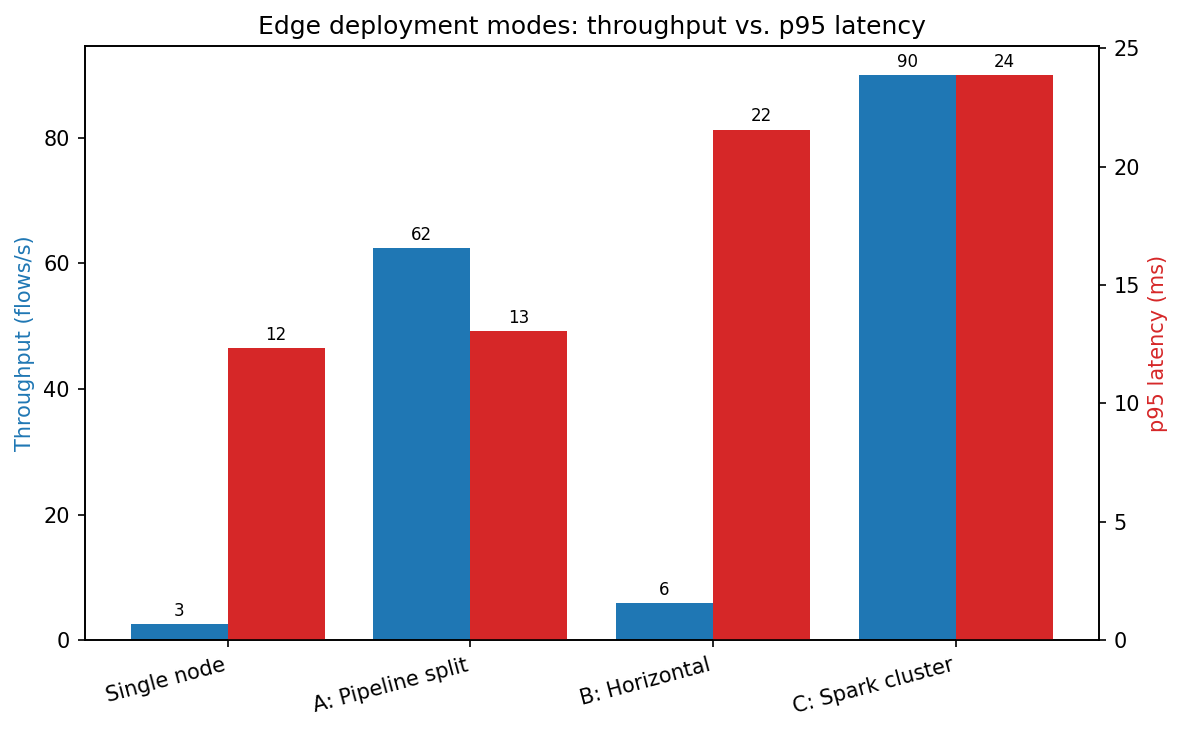
\includegraphics[width=0.95\textwidth]{img/edge_modes.png}}{\fbox{\parbox{0.8\textwidth}{\centering\vspace{1.2cm}\ph{Biểu đồ so sánh chế độ triển khai --- chạy plot\_edge\_modes.py}\vspace{1.2cm}}}}
    \caption[Thông lượng và độ trễ p95 của bốn cấu hình triển khai]{Thông lượng và độ trễ p95 của bốn cấu hình (một nút cơ sở + ba chế độ phân tán) trên cụm 2 Jetson}
    \label{fig:edge_modes}
\end{figure}

Kết quả thực đo (Hình~\ref{fig:edge_modes}) cho thấy: chế độ \emph{pipeline split} tách cổng khỏi bộ phân loại Spark giúp thông lượng phán quyết tăng từ 2{,}6 lên 62{,}5 luồng/giây (gấp $\approx$24 lần) với p95 gần như không đổi, nhờ cổng lọc 95{,}8\% lưu lượng bình thường và không còn bị Spark chặn vòng xử lý. \emph{Mở rộng theo chiều ngang} chỉ tăng xấp xỉ gấp đôi một nút (5{,}9 so với 2{,}6) vì mỗi nút vẫn chạy trọn bộ phân loại Spark trong tiến trình. \emph{Spark cluster} (cổng + bộ phân loại nối cụm Spark standalone) đạt thông lượng trung bình cao nhất (90{,}0) nhưng dao động lớn giữa các lần chạy ($\pm$26) và phụ thuộc thêm nút chủ (master) trên máy điều phối, nên pipeline split vẫn là khuyến nghị mặc định. \emph{Năng lượng mỗi suy luận} đo bằng \texttt{tegrastats} (nền idle 30\,giây trước mỗi cửa sổ tải; chế độ hai nút cộng công suất cả hai bo mạch): ở mức tải 100 luồng/giây, phần công suất \emph{hoạt động} (đã trừ idle) nằm dưới ngưỡng nhiễu lấy mẫu ($<$0{,}15\,W mọi nút), do đó bảng báo cáo năng lượng \emph{toàn bo mạch} trên mỗi phán quyết, tức thước đo mức dàn trải công suất bo mạch theo thông lượng ở cấp triển khai (không phải chi phí riêng của mô hình): các chế độ dùng cổng (A, C) dàn trải công suất hai bo mạch trên số phán quyết lớn gấp 24--35 lần, giảm năng lượng mỗi phán quyết từ $\approx$2{,}5\,J xuống 0{,}12--0{,}18\,J.

\pagebreak

\subsection{Phân tích và lựa chọn mô hình}

Hình~\ref{fig:benchmark_comparison} minh họa trực quan sự khác biệt giữa ba mô hình về thông lượng, độ trễ và mức sử dụng RAM trên Jetson Orin Nano Super.

\begin{figure}[htbp]
    \centering
    \IfFileExists{img/benchmark_comparison.png}{
\includegraphics[width=0.85\textwidth]{img/benchmark_comparison.png}}{\fbox{\parbox{0.8\textwidth}{\centering\vspace{1.4cm}\ph{Biểu đồ so sánh hiệu năng --- tạo từ \texttt{benchmark\_comparison.json}}\vspace{1.4cm}}}}
    \caption{So sánh hiệu năng ba mô hình trên Jetson Orin Nano Super}
    \label{fig:benchmark_comparison}
\end{figure}

Kết quả benchmark cho thấy sự đánh đổi rõ ràng giữa các chỉ số:

\begin{itemize}
    \item \textbf{Random Forest} thắng ở cả ba chỉ số vận hành quan trọng nhất với phát hiện xâm nhập thời gian thực: thông lượng cao nhất (26{,}8 mẫu/giây), độ trễ p95 thấp nhất (397\,ms) và CPU thấp nhất (35{,}2\%), nhờ Spark song song hóa tốt trên nhiều cây. Cái giá phải trả là RAM cao nhất (27{,}5\%) và mô hình lớn nhất ($\approx$4{,}4\,MB).
    \item \textbf{\ac{gbt}} có hiệu năng trung bình ở tất cả các chỉ số, đóng vai trò cầu nối giữa Decision Tree và Random Forest.
    \item \textbf{Decision Tree} nhẹ nhất về bộ nhớ (RAM 21{,}9\%, mô hình $\approx$0{,}05\,MB) nhưng chậm nhất: thông lượng 22{,}0 mẫu/giây và độ trễ p95 537\,ms, cao hơn Random Forest khoảng 35\%.
\end{itemize}

Hình~\ref{fig:model_tradeoff} thể hiện sự đánh đổi đa chiều giữa các tiêu chí lựa chọn mô hình: Decision Tree chiếm ưu thế về bộ nhớ, còn Random Forest chiếm ưu thế về tốc độ xử lý và tải CPU.

\begin{figure}[htbp]
    \centering
    \IfFileExists{img/model_tradeoff_radar.png}{
\includegraphics[width=0.75\textwidth]{img/model_tradeoff_radar.png}}{\fbox{\parbox{0.7\textwidth}{\centering\vspace{1.4cm}\ph{Biểu đồ radar trade-off --- tạo từ \texttt{benchmark\_comparison.json}}\vspace{1.4cm}}}}
    \caption[Biểu đồ radar đánh đổi giữa các mô hình trên thiết bị biên]{Biểu đồ radar thể hiện sự đánh đổi (trade-off) giữa các mô hình trên thiết bị biên}
    \label{fig:model_tradeoff}
\end{figure}

\textbf{Random Forest được chọn} làm mô hình triển khai chính trên thiết bị biên dựa trên ba tiêu chí:
\begin{enumerate}
    \item \textbf{Hiệu năng xử lý thời gian thực}: thông lượng cao nhất (26{,}8 mẫu/giây) và độ trễ p95 thấp nhất (397\,ms). Với \ac{ids}, độ trễ phán quyết là ràng buộc trực tiếp --- một mô hình nhỏ nhưng chậm hơn 35\% về p95 sẽ kéo dài cửa sổ mà tấn công chưa bị chặn.
    \item \textbf{Chất lượng phát hiện}: cao nhất trong ba mô hình ứng viên ở \emph{cả hai} phép đo --- F1 0{,}9955 trên đánh giá ngoại tuyến đầy đủ (Bảng~\ref{tab:summary_comparison}) và 0{,}9826 ở bản xuất huấn luyện trên mẫu con để vừa bộ nhớ một nút (Bảng~\ref{tab:edge_training}).
    \item \textbf{Tương thích nền tảng}: Random Forest là estimator gốc của Spark ML nên \texttt{PipelineModel} xuất ra nạp được trực tiếp trên bo mạch ARM64, không cần các thư viện native mà tích hợp \ac{xgb} của Spark đòi hỏi.
\end{enumerate}

Đánh đổi được chấp nhận là mức tiêu thụ bộ nhớ: Random Forest dùng 27{,}5\% RAM so với 21{,}9\% của Decision Tree và mô hình nặng $\approx$4{,}4\,MB so với 0{,}05\,MB. Trên bo mạch 8\,GB, khoảng chênh này còn dư địa lớn, nên bộ nhớ không phải là ràng buộc quyết định; Decision Tree vẫn là phương án dự phòng hợp lý nếu triển khai xuống các thiết bị \ac{iot} eo hẹp bộ nhớ hơn.

\section{Thảo luận và So sánh tổng hợp}
Kết quả thực nghiệm cho thấy lựa chọn đặc trưng dựa trên \ac{shap} là hướng tiếp cận phù hợp cho hệ thống \ac{ids} trên bộ dữ liệu CICIDS2017: dưới cấu hình đánh giá loại trừ rò rỉ dữ liệu, \ac{shap} Top-30 giữ được hiệu năng gần như nguyên vẹn trong khi cắt khoảng 60\% số đặc trưng. Ngược lại, học tổ hợp \emph{không} mang lại lợi thế trên chính cấu hình này: Hybrid Bagging đạt F1 0{,}9966 và Soft Voting đạt 0{,}9967, đều \emph{thấp hơn} \ac{xgb} đơn lẻ (0{,}9970). Học tổ hợp chỉ vượt mô hình đơn ở những cấu hình mà mô hình đơn yếu hơn (\ac{rf} Top-30: 0{,}9938 so với 0{,}9922; \ac{pca} $k$=40: 0{,}9940 so với 0{,}9939), nghĩa là nó \emph{bù cho bộ đặc trưng kém} chứ không tạo thêm hiệu năng phân loại. Chi phí đi kèm lại lớn: trên \ac{shap} Top-30, Hybrid Bagging cần 4909\,giây huấn luyện (so với 1226\,giây của \ac{xgb}), 46{,}6\,giây dự đoán (so với 7{,}1\,giây) và mô hình nặng 7{,}15\,MB --- lớn nhất trong tất cả các cấu hình đã thử. Vì vậy cấu hình được chọn để triển khai lên thiết bị biên là một \emph{mô hình đơn} trên tập đặc trưng \ac{shap} Top-30, không phải mô hình học tổ hợp.

Đặc biệt, khi triển khai trên thiết bị biên Jetson Orin Nano Super, Random Forest với SHAP Top-30 đặc trưng đạt F1-Score 0{,}9955 ngoại tuyến (đã loại trừ rò rỉ), thông lượng 26{,}8 mẫu/giây, độ trễ p95 397\,ms và sử dụng 27{,}5\% RAM. Các số liệu này cho phép đánh giá tính khả thi của việc triển khai hệ thống IDS dựa trên học máy trên các thiết bị biên có tài nguyên giới hạn, mở ra hướng ứng dụng thực tế cho giám sát an ninh mạng phân tán.







\chapter{Kết luận và hướng phát triển}
\label{c:ketluanvaphattrien}
Trong chương này, luận văn sẽ trình bày những kết quả mà luận văn đã đạt được so với mục tiêu được đặt ra từ ban đầu khi bắt đầu thực hiện. Bên cạnh đó, luận văn cũng trình bày những hạn chế và đưa ra hướng phát triển trong tương lai của nghiên cứu.

\section{Những đóng góp chính của luận văn}
Sau khi thực hiện luận văn với đề tài \textit{``Phát hiện xâm nhập (\ac{ids}) dựa trên Apache Spark cho bảo mật mạng \ac{iot}''}, luận văn đã đạt được một số kết quả chính tương ứng với các mục tiêu đề ra ban đầu:
\begin{itemize}
    \item \textbf{Xây dựng nền tảng xử lý dữ liệu lớn}: Đề xuất và triển khai thành công hệ thống \ac{ids} trên nền tảng Apache Spark. Giải pháp này tận dụng khả năng tính toán song song để xử lý các luồng dữ liệu mạng quy mô lớn từ môi trường \ac{iot}, đảm bảo tính mở rộng và hiệu năng cao trong việc giám sát bảo mật.
    \item \textbf{Cải thiện hiệu năng phát hiện với mô hình Ensemble}: Phát triển mô hình Hybrid Bagging Ensemble kết hợp đa thuật toán (Random Forest, \ac{xgb}, MLP). Dưới quy trình đánh giá loại trừ rò rỉ dữ liệu, mô hình đạt F1-score \ph{} (điền sau khi chạy lại) và được so sánh với các mô hình đơn lẻ kèm kiểm định ý nghĩa thống kê để khẳng định khác biệt (nếu có) là đáng kể.
    \item \textbf{Đánh giá trung thực, loại trừ rò rỉ dữ liệu}: Nhận diện và xử lý các nguồn rò rỉ thường gặp trên CIC-\ac{ids}2017 (đặc trưng \texttt{destination\_port} rò rỉ nhãn và trùng lặp luồng ở mức đặc trưng), đồng thời định lượng mức thổi phồng hiệu năng do rò rỉ — giúp kết quả phản ánh đúng năng lực thực của mô hình.
    \item \textbf{Tối ưu hóa và Giải thích mô hình}: Ứng dụng kỹ thuật \ac{shap} để lựa chọn các đặc trưng quan trọng nhất, giúp giảm số lượng đặc trưng (khoảng 60\%) trong khi giữ phần lớn hiệu năng phân loại. Đồng thời, \ac{shap} cung cấp khả năng giải thích chi tiết về quyết định của mô hình, tăng cường độ tin cậy và khả năng ứng dụng thực tế.
\end{itemize}

\section{Hạn chế của đề tài}
Mặc dù đã đạt được các kết quả nêu trên, luận văn vẫn còn một số hạn chế cần được khắc phục trong các giai đoạn tiếp theo:
\begin{itemize}
    \item \textbf{Phạm vi phân loại}: Hệ thống triển khai chính dựa trên bài toán phân loại nhị phân (Tấn công so với Bình thường); luận văn đã bổ sung đánh giá đa lớp theo từng loại tấn công (Mục~\ref{sec:multiclass}) để phân tích điểm yếu ở các lớp hiếm, song việc xây dựng một bộ phân loại đa lớp hoàn chỉnh cho triển khai realtime vẫn là hướng phát triển tiếp theo.
    \item \textbf{Môi trường triển khai}: Hệ thống được huấn luyện phân tán trên cụm Spark gồm máy chủ Mac và hai nút Jetson Orin Nano Super Developer Kit (8\,GB), và chính hai thiết bị này cũng được dùng để triển khai, đo hiệu năng thực tế ở pha suy luận; tuy nhiên việc kiểm chứng trên hạ tầng mạng \ac{iot} thực tế với hàng nghìn thiết bị đầu cuối và lưu lượng trực tuyến vẫn là thách thức cần thực hiện.
    \item \textbf{Phạm vi bộ dữ liệu}: Luận văn đã thiết lập quy trình đánh giá tổng quát hoá liên bộ dữ liệu (huấn luyện trên một bộ, kiểm tra trên bộ khác --- Mục~\ref{sec:cross-dataset}) trên cặp CIC-\ac{ids}2017 và CSE-CIC-IDS2018; việc mở rộng sang nhiều bộ mới hơn (CIC-IoT, RoEduNet) để củng cố kết luận về khái quát hoá vẫn là hướng tiếp theo.
\end{itemize}

\section{Hướng phát triển trong tương lai}
Dựa trên những kết quả đã đạt được và nhận diện các hạn chế hiện có, luận văn đề xuất một số hướng phát triển trong tương lai như sau:
\begin{itemize}
    \item \textbf{Nâng cấp khả năng nhận diện đa lớp}: Mở rộng mô hình để có thể phân loại chi tiết các loại tấn công phổ biến trong mạng \ac{iot} như DoS/DDoS, Botnet (Mirai), Infiltration và Heartbleed.
    \item \textbf{Tích hợp học máy trực tuyến (Online Learning)}: Nghiên cứu các giải pháp cập nhật tham số mô hình theo thời gian thực (real-time stream processing) mà không cần huấn luyện lại toàn bộ dữ liệu, giúp hệ thống thích ứng nhanh với các biến thể tấn công mới.
\end{itemize}


\appendix
\renewcommand{\cftchappresnum}{Phụ lục }
\addtocontents{toc}{\protect\renewcommand{\protect\cftchappresnum}{Phụ lục }}
\chapter{Công trình khoa học đã công bố}
Phần này liệt kê bài báo khoa học liên quan đến đề tài luận văn (viết chung với ThS. Nguyễn Vũ Thái, TS. Đỗ Trí Nhựt và TS. Nguyễn Văn Dũ), bài báo đã được chấp nhận đăng:

\begin{enumerate}
  \item Thai Nguyen Vu, \textbf{Dung Van Bui}, Nhut Tri Do, Van Du Nguyen, ``A Comparison of Dimensionality Reduction and Feature Selection for Network Intrusion Detection on Apache Spark ML with a Leakage-Aware Evaluation Pipeline,'' National Conference on Fundamental and Applied Information Technology Research (FAIR), 2026.
\end{enumerate}

Hình~\ref{fig:fair_accept} là thư thông báo chấp nhận đăng bài của Ban tổ chức Hội nghị FAIR 2026.

\begin{figure}[htbp]
    \centering
    \IfFileExists{img/fair_2026_accept.png}{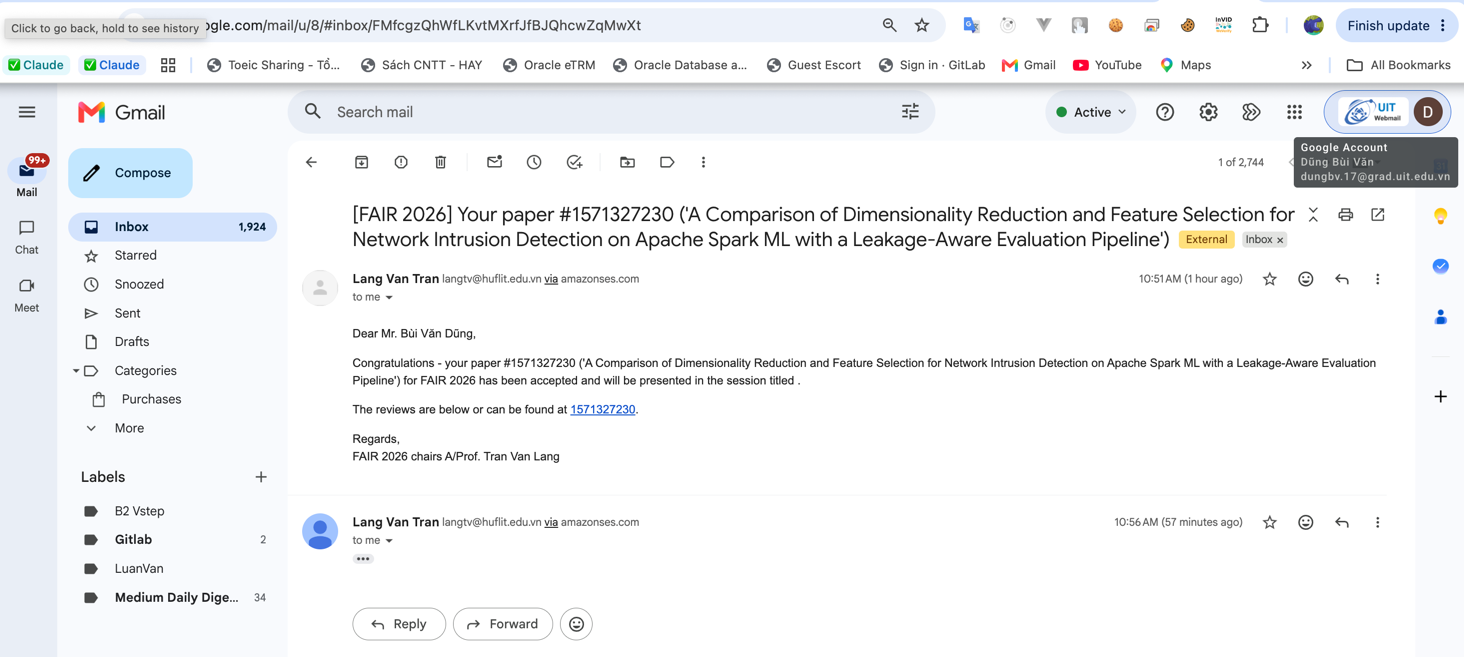
\includegraphics[width=\textwidth]{img/fair_2026_accept.png}}{\fbox{\parbox{0.85\textwidth}{\centering\vspace{1.2cm}\ph{Thư chấp nhận đăng bài của Hội nghị FAIR 2026}\vspace{1.2cm}}}}
    \caption[Thư chấp nhận đăng bài của Hội nghị FAIR 2026]{Thư thông báo chấp nhận đăng bài (paper \#1571327230) của Ban tổ chức Hội nghị FAIR 2026}
    \label{fig:fair_accept}
\end{figure}

Bản PDF đầy đủ của bài báo được đính kèm ở cuối luận văn, sau phần Tài liệu tham khảo.

\begingroup
\setlength{\emergencystretch}{8em}
\justifying\printbibliography[title=Tài liệu tham khảo]
\endgroup
\addcontentsline{toc}{chapter}{Tài liệu tham khảo}



\end{document}
